% =====================================================================
%  PoCAT Lektron SW: Docker and test infrastructure. Complete guide.
%  Study document and figure source for the team (Nanosatlab, UPC).
%
%  Build (Docker, nothing to install on the PC), from the repository root:
%    PowerShell:  & "C:\Program Files\Git\bin\bash.exe" docs/testing/overview/build-docs.sh
%    Git Bash:    bash docs/testing/overview/build-docs.sh
%  build-docs.sh runs the host tests (generated/test-results.tex), exports the
%  draw.io figures (figures/*.drawio -> figures/pdf/*.pdf) and typesets this
%  file with Tectonic. See the appendix "Rebuilding this document".
%  Close the PDF in the viewer before rebuilding: Windows locks the open file.
%
%  The test numbers (\TR... macros) come from the latest run. The prose was
%  verified against the repo on 2026-11-13 (branch obdh-compression,
%  HEAD b233846 + uncommitted changes). The Catalan original of this guide
%  is docker-and-test-guide-ca.tex.
% =====================================================================
\documentclass[11pt,a4paper]{article}

% Tectonic compiles with XeTeX: OpenType fonts with full Unicode.
\usepackage{fontspec}
\usepackage[english]{babel}
\setmainfont{texgyreheros}[Extension=.otf, UprightFont=*-regular, BoldFont=*-bold,
  ItalicFont=*-italic, BoldItalicFont=*-bolditalic]
\setsansfont{texgyreheros}[Extension=.otf, UprightFont=*-regular, BoldFont=*-bold,
  ItalicFont=*-italic, BoldItalicFont=*-bolditalic]
\setmonofont{DejaVuSansMono}[Extension=.ttf, BoldFont=*-Bold, ItalicFont=*-Oblique,
  BoldItalicFont=*-BoldOblique, Scale=0.86]
\usepackage[a4paper,margin=1.8cm,headheight=14pt]{geometry}
\usepackage{xcolor}
\usepackage{tikz}
\usetikzlibrary{positioning,fit,arrows.meta,calc,backgrounds,shapes.geometric}
\usepackage{pdflscape}
\usepackage{booktabs,tabularx,longtable,array,multirow}
\usepackage{enumitem}
\usepackage{caption}
\usepackage{float}
\usepackage{fancyhdr}
\usepackage{listings}
\usepackage{graphicx}
\usepackage[hidelinks]{hyperref}

\setlist{itemsep=2pt,topsep=4pt}
\setlength{\parindent}{0pt}
\setlength{\parskip}{5pt}
\setlength{\emergencystretch}{3em}
\captionsetup{font=small,labelfont=bf,margin=0pt,justification=raggedright,singlelinecheck=false}

% ---------------------------------------------------------------- inline code
% \_ allows a line break after the underscore (long identifiers in tables).
\DeclareRobustCommand{\_}{\textunderscore\allowbreak}
\newcommand{\cd}[1]{\texttt{#1}}
\newcommand{\PWD}{\$\{PWD\}}
\newcommand{\fl}{\ensuremath{\rightarrow}}

\lstset{basicstyle=\ttfamily\small,columns=fullflexible,keepspaces=true,
        frame=single,rulecolor=\color{black!40},backgroundcolor=\color{black!3},
        xleftmargin=4pt,xrightmargin=4pt,aboveskip=6pt,belowskip=6pt,
        showstringspaces=false,upquote=false,breaklines=true,breakatwhitespace=false,breakindent=1.5em}
% Real terminal output: smaller font and a slightly darker background.
\lstdefinestyle{out}{basicstyle=\ttfamily\footnotesize,backgroundcolor=\color{black!7}}

% ---------------------------------------------------------------- palette
% Designed to be readable in grayscale too: each category has a different lightness
% and also a different border type (thick / thin / dashed).
\definecolor{cProdD}{HTML}{1F4E79}   % dark blue: production code borders
\definecolor{cProdL}{HTML}{DCE8F4}   % very light blue: production code
\definecolor{cFakeD}{HTML}{8A5200}   % dark ochre: fake borders
\definecolor{cFakeL}{HTML}{F0B65E}   % medium ochre: test fakes
\definecolor{cGrey}{HTML}{555555}
\definecolor{cBg}{HTML}{F1F1F1}
\definecolor{cCovFull}{HTML}{2B6596} % coverage: has a suite (dark)
\definecolor{cCovPart}{HTML}{A7C6E2} % coverage: partial (medium)
\definecolor{cWarn}{HTML}{9E2A2B}    % decision / warning marks

\tikzset{
  every node/.style={font=\sffamily},
  box/.style={draw, rounded corners=2pt, align=center, inner sep=4pt, minimum height=8mm, line width=0.7pt},
  prod/.style={box, fill=cProdL, draw=cProdD, line width=1.2pt},
  real/.style={box, fill=white, draw=black!80, line width=0.9pt},
  fake/.style={box, fill=cFakeL, draw=cFakeD, line width=0.9pt},
  stub/.style={box, fill=white, draw=cFakeD, dashed, line width=0.9pt},
  ghost/.style={box, fill=white, draw=black!35, dash pattern=on 2pt off 2pt, text=black!55, line width=0.6pt},
  tool/.style={box, fill=cBg, draw=cGrey},
  img/.style={box, fill=black!14, draw=black!75, line width=1pt},
  outp/.style={box, fill=white, draw=black!75, line width=1pt, double, double distance=1pt},
  head/.style={align=center, font=\sffamily\bfseries\large},
  note/.style={align=left, font=\sffamily\small, text=black!75},
  arr/.style={-{Stealth[length=2.6mm,width=2mm]}, line width=0.9pt, draw=black!75},
  darr/.style={arr, dashed},
  container/.style={draw=black!60, fill=black!4, rounded corners=4pt, line width=0.8pt, inner sep=3mm},
  covfull/.style={box, fill=cCovFull, draw=black!85, text=white, line width=0.9pt},
  covpart/.style={box, fill=cCovPart, draw=black!85, line width=0.9pt},
  covnone/.style={box, fill=white, draw=black!85, dashed, line width=0.9pt},
  hw/.style={box, fill=black!8, draw=black!50, line width=0.6pt, font=\sffamily\itshape},
  decision/.style={diamond, aspect=2.4, draw=black!80, fill=white, line width=0.9pt, align=center, inner sep=0pt, text width=3.3cm, font=\sffamily\small},
  card/.style={box, fill=white, draw=black!70, align=left, text width=5.3cm, font=\sffamily\small, inner sep=5pt},
  deccard/.style={card, draw=cWarn, line width=1.6pt},
  tag/.style={fill=cWarn, text=white, font=\sffamily\bfseries\scriptsize, inner sep=2pt, rounded corners=1pt},
  tagu/.style={fill=black!70, text=white, font=\sffamily\bfseries\scriptsize, inner sep=2pt, rounded corners=1pt},
  lbl/.style={font=\sffamily\small\bfseries, fill=white, inner sep=1.5pt},
}

% ---------------------------------------------------------------- headers
\pagestyle{fancy}
\fancyhf{}
\fancyhead[L]{\small PoCAT Lektron SW · Docker and test infrastructure}
\fancyhead[R]{\small\nouppercase{\leftmark}}
\fancyfoot[C]{\small\thepage}
\renewcommand{\headrulewidth}{0.4pt}
\fancypagestyle{plain}{\fancyhf{}\fancyfoot[C]{\small\thepage}\renewcommand{\headrulewidth}{0pt}}

% Large full-page figure, landscape (can be projected like a slide).
\newenvironment{slidefig}{\begin{landscape}\thispagestyle{plain}\begin{figure}[p]\centering}{\end{figure}\end{landscape}}

% Short warning box.
\newcommand{\avis}[2]{\par\smallskip\noindent\fcolorbox{cWarn}{white}{\parbox{\dimexpr\linewidth-2\fboxsep-2\fboxrule\relax}{\small\textbf{#1}\ #2}}\par\smallskip}

% ---------------------------------------------------------------- draw.io figures
% Exported by build-docs.sh from figures/*.drawio. If an export is missing
% (e.g. compiling with plain tectonic), a framed placeholder is printed instead
% of stopping the build.
\newcommand{\drawio}[2][\linewidth]{%
  \IfFileExists{figures/pdf/#2.pdf}%
    {\includegraphics[width=#1,height=0.80\textheight,keepaspectratio]{figures/pdf/#2.pdf}}%
    {\fbox{\parbox{0.6\linewidth}{\centering\small Figure \cd{figures/#2.drawio} not exported yet:\\run \cd{build-docs.sh}.}}}}

% ---------------------------------------------------------------- test results
% generated/test-results.tex is written by tools/collect-test-results.sh (run by
% build-docs.sh) from a real run of every suite. It defines \TRdate, \TRcommit,
% \TRsuites, \TRsuitesGreen, \TRsuitesCrashed, \TRtests, \TRpassed, \TRfailed,
% \TRignored and the table bodies \TRsuiteRows, \TRfailRows, \TRignoreRows.
% Without it the document still compiles and shows "?" instead of numbers.
\def\TRdate{(no run yet)}\def\TRcommit{?}
\def\TRsuites{?}\def\TRsuitesGreen{?}\def\TRsuitesCrashed{0}
\def\TRtests{?}\def\TRpassed{?}\def\TRfailed{?}\def\TRignored{?}
\def\TRsuiteRows{\multicolumn{6}{@{}l}{\emph{No test run found: run build-docs.sh.}}\\}
\def\TRfailRows{\multicolumn{3}{@{}l}{\emph{No test run found.}}\\}
\def\TRignoreRows{\multicolumn{3}{@{}l}{\emph{No test run found.}}\\}
\IfFileExists{generated/test-results.tex}{\input{generated/test-results.tex}}{}

\begin{document}

% =====================================================================
\begin{titlepage}
\centering
\vspace*{2.2cm}
{\Huge\bfseries Docker and test infrastructure\\[6pt] of PoCAT Lektron\par}
\vspace{0.8cm}
{\Large What was built, how to use it and how it works inside\par}
\vspace{2.5cm}

\begin{minipage}{0.86\textwidth}
\small
\textbf{What it covers.} All the work done since the first \cd{Dockerfile} (September 2026)
up to today: the two Docker images, the build and flash scripts, the
VS Code integration and the host test infrastructure (\TRsuites{} suites, \TRtests{} tests).
It does not cover only the last commit: it covers everything that exists, committed or not.

\medskip
\textbf{How it is organized.} Part~I (sections 1 and 2) gives the full picture and the
parts. Part~II (3 to 6) is the four workflows, step by step: build,
flash and debug, run tests, and the day-to-day routine. Part~III (7 to 10) explains how
the tests work inside, following one real test call by call. Part~IV
(11 to 13) is the catalog: suites, known problems, weak points and roadmap.
At the end there is a one-page command cheat sheet.

\medskip
\textbf{Figures.} The large figures are on their own landscape pages and can be
projected on their own: the caption of each figure says what to take away from it.

\medskip
\textbf{Sources.} Everything was checked against the repository code. The terminal
outputs shown are real, from the run of 13/11/2026. The test counts in the summary
are regenerated from a real run every time the PDF is built (appendix~\ref{sec:rebuild}). When something
could not be verified, the text says so. Code names, files and commands are
left as they are, in \cd{monospace}.
\end{minipage}
\vfill
\end{titlepage}

\tableofcontents
\clearpage
% =====================================================================
\part{The full picture}

\section{One-page summary}\label{sec:resum}

\begin{center}
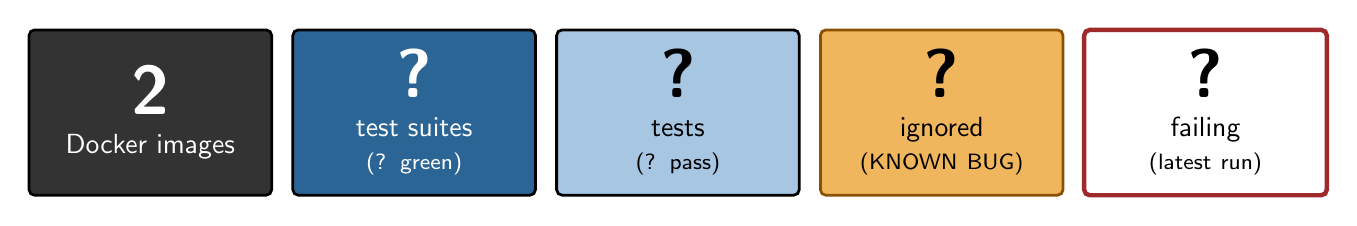
\begin{tikzpicture}[tile/.style={box, minimum width=3.05cm, minimum height=2.1cm, text width=2.8cm, line width=1pt}]
\node[tile, fill=black!80, text=white] (a) at (0,0)    {{\fontsize{24}{26}\selectfont\bfseries 2}\\[2pt] Docker images};
\node[tile, fill=cCovFull, text=white] (b) at (3.35,0) {{\fontsize{24}{26}\selectfont\bfseries \TRsuites}\\[2pt] test suites\\{\footnotesize (\TRsuitesGreen{} green)}};
\node[tile, fill=cCovPart] (c) at (6.7,0)  {{\fontsize{24}{26}\selectfont\bfseries \TRtests}\\[2pt] tests\\{\footnotesize (\TRpassed{} pass)}};
\node[tile, fill=cFakeL, draw=cFakeD] (d) at (10.05,0) {{\fontsize{24}{26}\selectfont\bfseries \TRignored}\\[2pt] ignored\\{\footnotesize (KNOWN BUG)}};
\node[tile, fill=white, draw=cWarn, line width=1.6pt] (e) at (13.4,0) {{\fontsize{24}{26}\selectfont\bfseries \TRfailed}\\[2pt] failing\\{\footnotesize (latest run)}};
\end{tikzpicture}

{\small Test numbers from the latest run: \TRdate{}, commit \cd{\TRcommit}.}
\end{center}

\textbf{The starting problem.} The PoCAT Lektron flight software is C on
FreeRTOS for an STM32L476RG. Before this work, building it required installing the
ARM toolchain on every computer (with different versions and paths on each one), and the only
way to test a change was to flash the board and see what happened.

\textbf{What was built.} Three things, which can be seen together in figure~\ref{fig:bigpicture}:
\begin{enumerate}
\item \textbf{Reproducible build.} The Docker image \cd{pocat-build-env} carries the
  ARM toolchain inside. A single command produces \cd{build/pocat\_lektron\_sw.elf}, the same on
  any PC (section~\ref{sec:build}).
\item \textbf{Host tests.} The \cd{pocat-tests} image compiles \emph{the same flight
  \cd{.c} files} with the PC's \cd{gcc} and replaces everything that depends on hardware
  (FreeRTOS, HAL, flash, radio) with test parts. Today there are \TRsuites{} suites with \TRtests{} tests,
  which run in one second and without a board (sections~\ref{sec:runtests} to~\ref{sec:fakes}).
\item \textbf{Flashing and debugging.} \cd{flash.sh} flashes the ELF to the Nucleo and finds the
  installed tool by itself, and VS Code does it with a button: shared tasks and debugging with
  \cd{F5} (section~\ref{sec:flash}).
\end{enumerate}

\textbf{State today.}
\begin{itemize}
\item \textbf{Latest run (\TRdate):} \TRsuitesGreen{} of \TRsuites{} suites green, \TRtests{} tests:
  \TRpassed{} pass, \TRfailed{} fail, \TRignored{} ignored. On 13/11/2026 the only failing suite was \cd{test\_ht\_handling}, with two tests
  that fail on purpose (KI-10 and KI-11); while they fail, the exit code of a full run is never 0.
\item The tests have found and documented 26 problems in the flight code (section~\ref{sec:ki}).
  None has been fixed from the tests: that is the project rule.
\item The firmware compiles (82\,392 bytes of code), and it can be flashed and it stops at \cd{main()} with \cd{F5}.
\item \textbf{Only 5 of the 15 suites are committed.} The rest of the work is only on disk.
\item The remote has 2 new commits (\emph{Flash step 1}) that change the flash API. When
  you do \cd{git pull}, fakes and tests will need to be adapted (section~\ref{sec:roadmap}).
\end{itemize}

\textbf{The four commands you need to know} (PowerShell, at the repo root, with Docker Desktop open):
\begin{lstlisting}
docker run --rm -v "${PWD}:/app" pocat-build-env      # build the firmware
docker run --rm -v "${PWD}:/app" pocat-tests           # run all tests
docker run --rm -v "${PWD}:/app" pocat-tests test_state_machine -f NM_to_SM
& "C:\Program Files\Git\bin\bash.exe" flash.sh         # flash the board
\end{lstlisting}
The images are built only once (section~\ref{sec:peces}). The full cheat sheet is in
appendix~\ref{sec:xuleta}.

% ---------------------------------------------------------------- FIGURE: full picture
\begin{slidefig}
\drawio[\linewidth]{docker-containers}
\caption{The full picture: the Docker containers (draw.io: \cd{figures/docker-containers.drawio}).
\textbf{What to take away:} there is one repository and two ways to build it. On top (blue), the path
to the board: ARM firmware, flashing and debugging. In the middle (ochre), the verification path: the
same code compiled for the PC and run against test parts, with no hardware. At the bottom (dashed),
the containers that only build this document. The repository is mounted into every container, never
copied, and the outputs end up in repository folders that git ignores.}
\label{fig:bigpicture}
\end{slidefig}

\clearpage
% =====================================================================
\section{The parts: files and Docker images}\label{sec:peces}

\subsection{Which file does what}

\begingroup
\small
\renewcommand{\arraystretch}{1.15}
\begin{longtable}{@{}>{\raggedright\arraybackslash}p{4.3cm}>{\raggedright\arraybackslash}p{9.6cm}>{\raggedright\arraybackslash}p{2.6cm}@{}}
\toprule
File & What it does & Status\\
\midrule
\endhead
\bottomrule
\endfoot
\cd{Dockerfile} & Recipe for the \cd{pocat-build-env} image: Ubuntu 22.04, \cd{cmake}, \cd{make}, \cd{git},
  \cd{python3} and the Arm GNU Toolchain 13.2.rel1 at \cd{/opt/arm-gcc}. Sets a development PSK and ends with
  \cd{CMD ["bash","build.sh"]}. & commit (v1.0)\\
\cd{build.sh} & Builds the firmware: generates \cd{psk.h} from \cd{POCAT\_PSK}, configures CMake with the
  ARM toolchain and calls \cd{make}. Flags \cd{--mock}, \cd{--clean}, \cd{--test-instr}. & commit (already existed)\\
\cd{Dockerfile.test} & Recipe for the \cd{pocat-tests} image: Ubuntu 22.04, \cd{build-essential} (native gcc) and
  \cd{cmake}. Ends with \cd{ENTRYPOINT ["bash","run\_tests.sh"]}. & commit (v2.0)\\
\cd{run\_tests.sh} & Configures \cd{build\_test/} with \cd{-DBUILD\_TESTING=ON}, builds the \cd{pocat\_tests} target and
  runs \cd{ctest} or a suite, depending on the arguments. 18 lines. & commit (v2.1)\\
\cd{CMakeLists.txt} (root) & Has two points that make the host test possible: if \cd{BUILD\_TESTING} is on it does not
  load the ARM toolchain, and at the end it does \cd{add\_subdirectory(test)}. & commit (v2.0)\\
\cd{test/CMakeLists.txt} & Defines \cd{pocat\_add\_suite()} and registers the suites, one line per suite. & commit, extended on disk\\
\cd{test/suites/} & The 15 suites, \cd{test\_<module>.c}. & 5 commit, 10 disk\\
\cd{test/mocks/}, \cd{test/support/} & Fakes, stubs and support (\cd{fake\_rtos}, \cd{fake\_link}, \cd{sim\_tasks}...). & part on disk\\
\cd{test/framework/unity/} & Unity, the test framework (third party, untouched). & commit (v2.0)\\
\cd{test/README.md} & Reference manual for the tests: commands, conventions R1--R6 and the table of known problems. & commit, extended on disk\\
\cd{docs/testing/*.md} & Design: \cd{test-design.md} (layers 1--4) and \cd{test-design-phase3.md} (specification of the latest suites). & part on disk\\
\cd{flash.sh} & Flashes \cd{build/pocat\_lektron\_sw.elf} to the Nucleo. Looks for the flashing tool in the \cd{PATH} and in
  the usual installation paths. & disk (rewritten)\\
\cd{.vscode/tasks.json} & Shared VS Code tasks: build, clean build, flash, build and flash, tests. & disk\\
\cd{.vscode/launch.json} & Debugging with \cd{F5} (Cortex-Debug + OpenOCD). Contains each person's PC paths: \textbf{it does not go to git}. & local\\
\cd{.gitattributes} & Forces LF line endings on \cd{*.sh} and \cd{Dockerfile*}, because \cd{bash} inside the container fails with CRLF. & disk\\
\cd{.gitignore} & Ignores \cd{build}, \cd{build\_test/}, \cd{psk.h} and \cd{.vscode/*} except \cd{tasks.json}. & disk\\
\end{longtable}
\endgroup

Figure~\ref{fig:tree} shows the same files as a tree, so you can see where each one lives.

\begin{figure}[p]
\centering
\drawio[0.97\linewidth]{repo-structure}
\caption{The repository after the Docker and test work (draw.io: \cd{figures/repo-structure.drawio}).
Colour = what kind of file it is; a dashed border = new or rewritten since the last commit
(\cd{b233846}). \textbf{What to take away:} the flight code (\cd{src/}, \cd{include/}) is untouched.
All the new test work lives under \cd{test/}, the Docker work is a handful of files at the root, and
everything generated (\cd{build/}, \cd{build\_test/}, \cd{generated/}) is ignored by git.}
\label{fig:tree}
\end{figure}

\subsection{The two images}

A Docker image is a ``snapshot'' of a system with the tools installed. It is built
once from a \cd{Dockerfile} and then containers are started from it; containers are
single-use copies: \cd{--rm} deletes them when they finish. The repository is not copied into the image:
it is \emph{mounted} with \cd{-v "\PWD:/app"}, so the container reads and writes
the PC folder directly.

\begin{lstlisting}
docker build -t pocat-build-env .                  # firmware image (2.16 GB)
docker build -t pocat-tests -f Dockerfile.test .   # tests image (641 MB)
\end{lstlisting}

You only need to rebuild them if the corresponding \cd{Dockerfile} changes. The firmware image takes
longer the first time because it downloads the ARM toolchain.

The two images end differently, and this has a practical consequence:
\begin{itemize}
\item \cd{pocat-tests} ends with \cd{ENTRYPOINT}: everything written after the name of
  the image goes straight to \cd{run\_tests.sh} (\cd{--list}, \cd{--label obc}, \cd{test\_obc -l}...).
\item \cd{pocat-build-env} ends with \cd{CMD}: what you write after it \emph{replaces}
  the command. To pass flags to \cd{build.sh} you must repeat the whole command:
  \cd{... pocat-build-env bash build.sh --clean}.
\end{itemize}

\textbf{The CMake hook.} The same \cd{CMakeLists.txt} serves both worlds. The
only lines that refer to it are these:
\begin{lstlisting}
if(NOT BUILD_TESTING)                       # lines 4-6
    set(CMAKE_TOOLCHAIN_FILE ${CMAKE_CURRENT_SOURCE_DIR}/cmake/toolchain.cmake)
endif()
...
option(BUILD_TESTING "Build unit tests (requires native compiler)" OFF)   # lines 175-179
if(BUILD_TESTING)
    enable_testing()
    add_subdirectory(test)
endif()
\end{lstlisting}
Without \cd{-DBUILD\_TESTING=ON}, the \cd{test/} folder does not exist for CMake and nothing in it
reaches the firmware. With the option on, CMake uses the native compiler and
adds the suites. That is why there are two separate output folders: \cd{build/}
(firmware) and \cd{build\_test/} (tests). Inside \cd{build\_test/} the default target
is still the firmware and it does not compile with native gcc: you must only build the
\cd{pocat\_tests} target, which is what \cd{run\_tests.sh} does.

% ---------------------------------------------------------------- FIGURE: pipelines
\begin{slidefig}
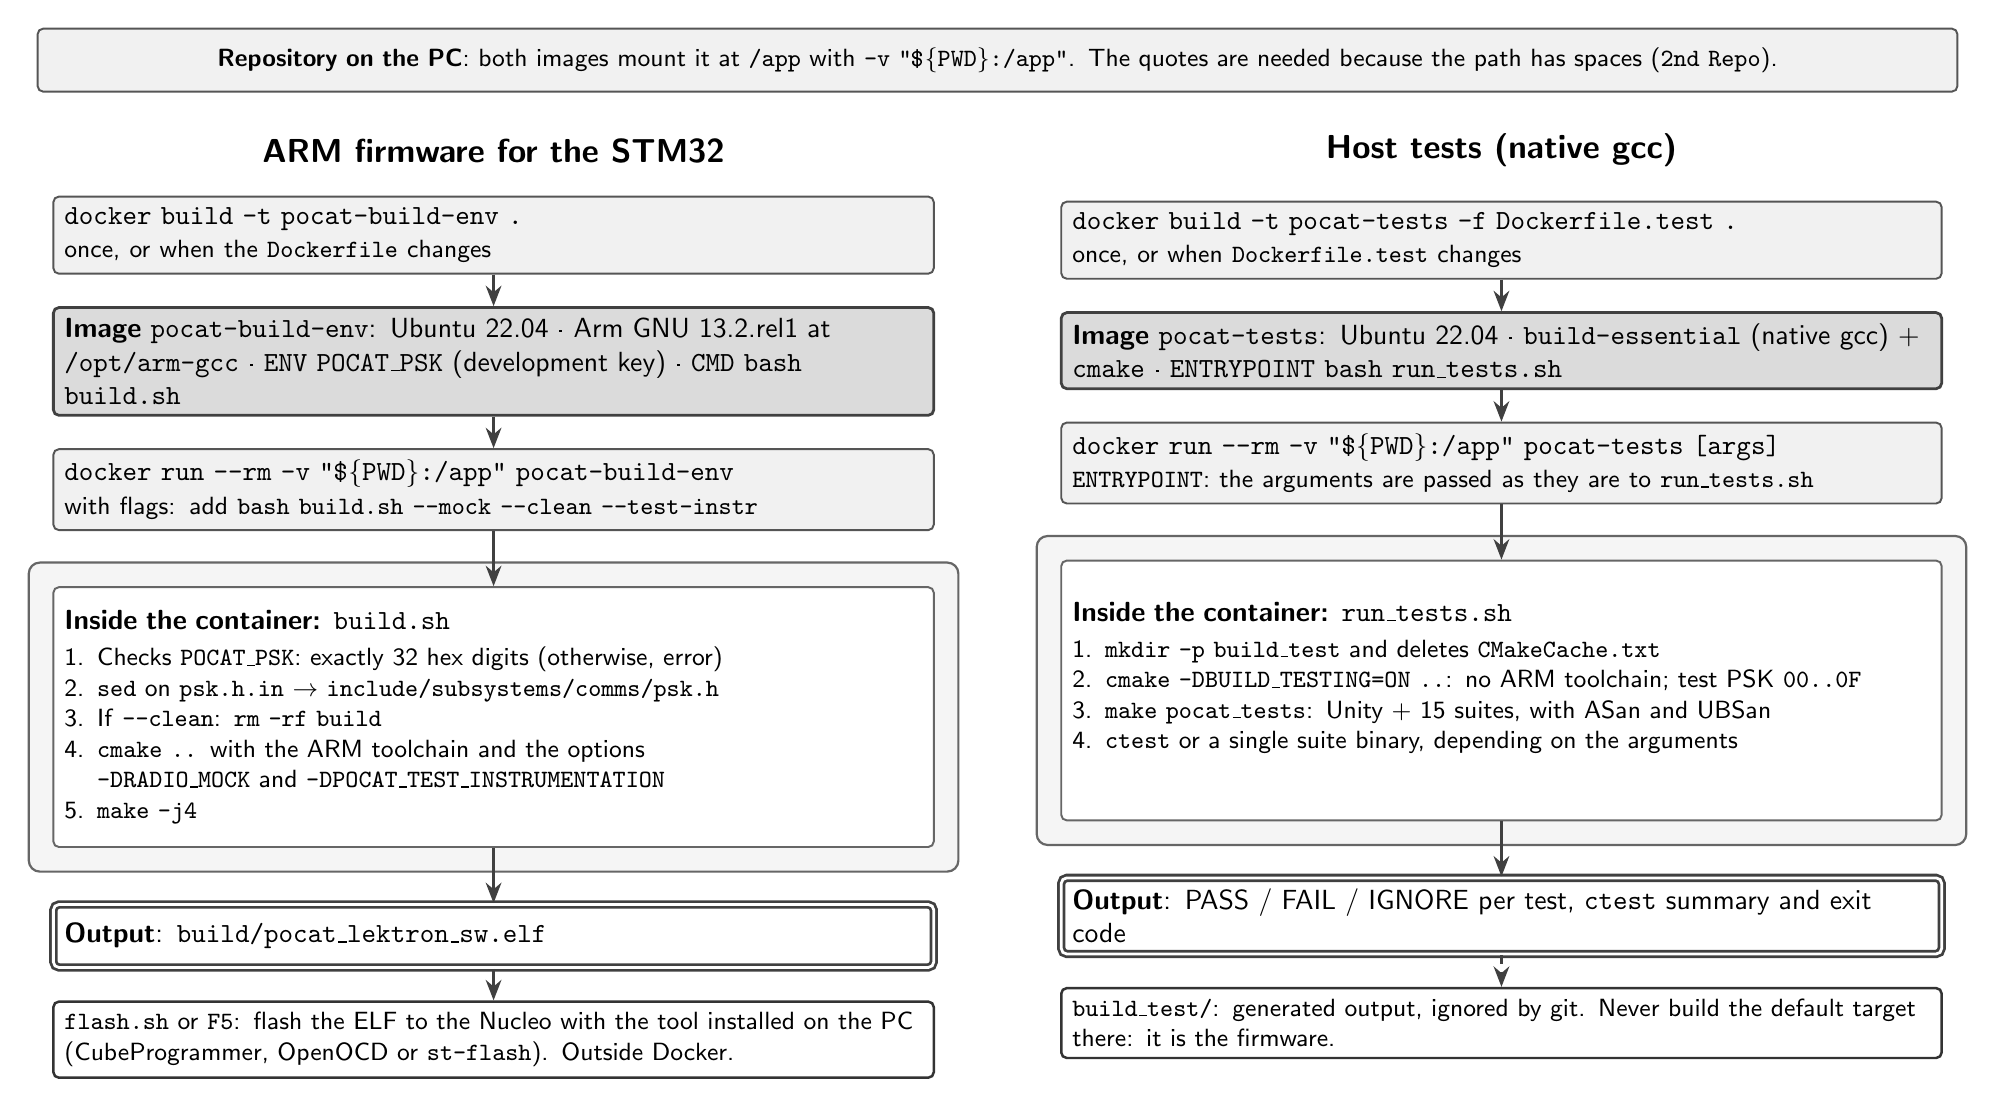
\begin{tikzpicture}[node distance=4mm,
  colbox/.style={text width=10.9cm, align=left},
  cmd/.style={tool, colbox},
  ]
\def\xL{5.9}\def\xR{18.7}
\node[tool, text width=24.1cm, align=center, font=\sffamily\small] (repo) at (12.3,0)
  {\textbf{Repository on the PC}: both images mount it at \cd{/app} with
   \cd{-v "\PWD:/app"}. The quotes are needed because the path has spaces (\cd{2nd Repo}).};

\node[head] (Lh) at (\xL,-1.15) {ARM firmware for the STM32};
\node[head] (Rh) at (\xR,-1.15) {Host tests (native gcc)};

% ---- left
\node[cmd, below=3mm of Lh] (L1) {\ttfamily docker build -t pocat-build-env .\\
  {\sffamily\small once, or when the \cd{Dockerfile} changes}};
\node[img, colbox, below=of L1] (L2) {\textbf{Image \cd{pocat-build-env}}: Ubuntu 22.04 · Arm GNU 13.2.rel1
  at \cd{/opt/arm-gcc} · \cd{ENV POCAT\_PSK} (development key) · \cd{CMD bash build.sh}};
\node[cmd, below=of L2] (L3) {\ttfamily docker run --rm -v "\PWD:/app" pocat-build-env\\
  {\sffamily\small with flags: add \cd{bash build.sh --mock --clean --test-instr}}};
\node[box, fill=white, draw=black!60, colbox, below=7mm of L3, font=\sffamily\small, minimum height=3.3cm] (L4)
  {\textbf{\normalsize Inside the container: \cd{build.sh}}\\[2pt]
   1. Checks \cd{POCAT\_PSK}: exactly 32 hex digits (otherwise, error)\\
   2. \cd{sed} on \cd{psk.h.in} \fl{} \cd{include/subsystems/comms/psk.h}\\
   3. If \cd{--clean}: \cd{rm -rf build}\\
   4. \cd{cmake ..} with the ARM toolchain and the options\\\phantom{4. }\cd{-DRADIO\_MOCK} and \cd{-DPOCAT\_TEST\_INSTRUMENTATION}\\
   5. \cd{make -j4}};
\node[outp, colbox, below=7mm of L4] (L5) {\textbf{Output}: \cd{build/pocat\_lektron\_sw.elf}};
\node[real, colbox, below=of L5, font=\sffamily\small] (L6) {\cd{flash.sh} or \cd{F5}: flash the ELF to the Nucleo with the tool
  installed on the PC (CubeProgrammer, OpenOCD or \cd{st-flash}). Outside Docker.};

% ---- right
\node[cmd, below=3mm of Rh] (R1) {\ttfamily docker build -t pocat-tests -f Dockerfile.test .\\
  {\sffamily\small once, or when \cd{Dockerfile.test} changes}};
\node[img, colbox, below=of R1] (R2) {\textbf{Image \cd{pocat-tests}}: Ubuntu 22.04 · \cd{build-essential} (native gcc)
  + \cd{cmake} · \cd{ENTRYPOINT bash run\_tests.sh}};
\node[cmd, below=of R2] (R3) {\ttfamily docker run --rm -v "\PWD:/app" pocat-tests [args]\\
  {\sffamily\small \cd{ENTRYPOINT}: the arguments are passed as they are to \cd{run\_tests.sh}}};
\node[box, fill=white, draw=black!60, colbox, below=7mm of R3, font=\sffamily\small, minimum height=3.3cm] (R4)
  {\textbf{\normalsize Inside the container: \cd{run\_tests.sh}}\\[2pt]
   1. \cd{mkdir -p build\_test} and deletes \cd{CMakeCache.txt}\\
   2. \cd{cmake -DBUILD\_TESTING=ON ..}: no ARM toolchain; test PSK \cd{00..0F}\\
   3. \cd{make pocat\_tests}: Unity + 15 suites, with ASan and UBSan\\
   4. \cd{ctest} or a single suite binary, depending on the arguments\\
   \phantom{5.}};
\node[outp, colbox, below=7mm of R4] (R5) {\textbf{Output}: PASS / FAIL / IGNORE per test, \cd{ctest} summary and exit code};
\node[real, colbox, below=of R5, font=\sffamily\small] (R6) {\cd{build\_test/}: generated output, ignored by git.
  Never build the default target there: it is the firmware.};

\begin{scope}[on background layer]
  \node[container, fit=(L4)] {};
  \node[container, fit=(R4)] {};
\end{scope}
\foreach \a/\b in {L1/L2,L2/L3,L3/L4,L4/L5,L5/L6,R1/R2,R2/R3,R3/R4,R4/R5}
  \draw[arr] (\a) -- (\b);
\draw[darr] (R5) -- (R6);
\end{tikzpicture}
\caption{The two Docker pipelines, step by step. \textbf{What to take away:} both columns follow the same
path (build the image, start a container with the repository mounted, run a script),
but the left one produces the ELF for the STM32 and needs the PSK, and the right one compiles with the PC's gcc and
runs the tests instantly. In the firmware image the flags go after \cd{bash build.sh}; in the
tests image they go directly after the image name.}
\label{fig:docker}
\end{slidefig}
% =====================================================================
\part{The workflows}

\section{Workflow 1: building the firmware}\label{sec:build}

\textbf{Requirements.} Docker Desktop open and the \cd{pocat-build-env} image built
(section~\ref{sec:peces}). Nothing else.

\textbf{The command}, from the root of the repository:
\begin{lstlisting}
docker run --rm -v "${PWD}:/app" pocat-build-env
\end{lstlisting}

\textbf{What happens, step by step} (left column of figure~\ref{fig:docker}):
\begin{enumerate}
\item Docker starts a container from the image and mounts the current folder at \cd{/app}.
\item The container runs \cd{bash build.sh}.
\item \cd{build.sh} reads the \cd{POCAT\_PSK} variable (the image ships with a development
  one). It must have exactly 32 hexadecimal digits (16 bytes); otherwise it stops
  with an error.
\item It converts the key into C bytes and, with \cd{sed}, generates
  \cd{include/subsystems/comms/psk.h} from the template \cd{psk.h.in}.
\item It creates \cd{build/}, runs \cd{cmake ..} there (which loads the ARM toolchain from
  \cd{cmake/toolchain.cmake}) and then \cd{make -j4}.
\item The result is \cd{build/pocat\_lektron\_sw.elf}, which stays in the folder on the PC because
  \cd{/app} is the mounted repository.
\end{enumerate}

\textbf{What comes out.} The ELF is the firmware with debug information (2.7\,MB on disk,
but only part of it goes to the board). The real size is shown with:
\begin{lstlisting}
docker run --rm -v "${PWD}:/app" pocat-build-env arm-none-eabi-size build/pocat_lektron_sw.elf
\end{lstlisting}
\begin{lstlisting}[style=out]
   text    data     bss     dec     hex filename
  82392     396   80240  163028   27cd4 build/pocat_lektron_sw.elf
\end{lstlisting}
\cd{text} is what takes up space in flash: 82\,392 bytes, 8\,\% of the megabyte of the STM32L476RG.
\cd{data} + \cd{bss} is the statically reserved RAM (80\,636 bytes), which includes the
FreeRTOS \emph{heap}. These numbers come from the build of 13/11/2026 with the local code
(without the new commits from the remote).

\begin{table}[H]
\centering\small
\begin{tabularx}{\textwidth}{@{}l>{\raggedright\arraybackslash}X@{}}
\toprule
\cd{build.sh} flag & Effect\\
\midrule
\cd{--clean} & Deletes \cd{build/} before building: full rebuild and a fresh CMake configuration.\\
\cd{--mock} & \cd{cmake -DRADIO\_MOCK=ON}: defines the \cd{RADIO\_MOCK} macro. The \cd{\#ifdef}s in the RadioLib wrappers
  leave only \cd{radiolib\_wrapper\_mock.c} active (simulated radio: it prints the configuration and the TX packets;
  reception always times out). \textbf{It probably does not compile} (KI-7); this has not been verified.\\
\cd{--test-instr} & \cd{cmake -DPOCAT\_TEST\_INSTRUMENTATION=ON}: uses TIM5 to measure, in microseconds, the computation of the authentication
  tag and the CAD scan, and prints the results. Only for bench test campaigns.\\
\bottomrule
\end{tabularx}
\caption{\cd{build.sh} flags. They can be combined. Because the image ends with \cd{CMD}, they must be passed like this:
\cd{docker run --rm -v "\PWD:/app" pocat-build-env bash build.sh --clean}.}
\end{table}

\textbf{The PSK.} This is the pre-shared key used to authenticate radio frames.
\cd{psk.h} is a generated file: do not edit it and do not commit it (it is in \cd{.gitignore}). The
image ships with the development key \cd{0123456789ABCDEF0123456789ABCDEF}; to build
with another one:
\begin{lstlisting}
docker run --rm -e POCAT_PSK=<32 hex digits> -v "${PWD}:/app" pocat-build-env
\end{lstlisting}
The tests do not use this key: they have their own (section~\ref{sec:idea}).

\begin{table}[H]
\centering\small
\begin{tabularx}{\textwidth}{@{}>{\raggedright\arraybackslash}p{5.6cm}>{\raggedright\arraybackslash}X>{\raggedright\arraybackslash}p{4.3cm}@{}}
\toprule
What you see & Why it happens & Fix\\
\midrule
\cd{CMake Error: The current CMakeCache.txt directory /app/build/... is different than the directory ...
where CMakeCache.txt was created} and \cd{/usr/bin/cmake.exe: not found} &
\cd{build/} contains a configuration made outside Docker (for example with \cd{cmake} from Git Bash on Windows), with the
paths of that environment. This happened on 13/11. & Build once with \cd{bash build.sh --clean}\\
\cd{\$'\textbackslash r': command not found} & The script has Windows line endings (CRLF) and Linux \cd{bash} does not understand them. &
Check that \cd{.gitattributes} is there and save the script with LF line endings\\
\cd{ERROR: POCAT\_PSK is not set} & \cd{build.sh} was run outside the image, or with an empty variable. & Define \cd{POCAT\_PSK} (32 hex digits)\\
\cd{failed to connect to the docker API at npipe:////./pipe/\allowbreak dockerDesktopLinuxEngine} & Docker Desktop is not running. & Open Docker Desktop and wait for it to start\\
\cd{Unable to find image 'pocat-build-env:latest' locally} & The image has not been built on this PC. & \cd{docker build -t pocat-build-env .}\\
\bottomrule
\end{tabularx}
\caption{Typical errors when building the firmware.}
\label{tab:builderrors}
\end{table}

\avis{Known weak point.}{\cd{run\_tests.sh} deletes \cd{CMakeCache.txt} on every run, which is why the tests
never suffer from the first error in the table. \cd{build.sh} does not do this. Adding the same line to it is a pending
improvement (section~\ref{sec:roadmap}).}

\clearpage
% =====================================================================
\section{Workflow 2: flashing, running and debugging on the board}\label{sec:flash}

Flashing means writing the firmware to the STM32 flash through the ST-LINK, the
debugger built into the Nucleo. This cannot be done from Docker on Windows (the
container cannot see USB), so it is done with a tool installed on the PC. There are three
ways, and they all end up doing the same thing:

\begin{table}[H]
\centering\small
\begin{tabularx}{\textwidth}{@{}>{\raggedright\arraybackslash}p{3.6cm}>{\raggedright\arraybackslash}X>{\raggedright\arraybackslash}p{4.4cm}@{}}
\toprule
Way & What it does & Who it is for\\
\midrule
\cd{bash flash.sh} & Flashes the ELF that is already built, verifies it and resets the board. & Everyone; it does not depend on any editor. It is in git.\\
VS Code task & \emph{PoCAT: flash Nucleo} calls \cd{flash.sh}; \emph{PoCAT: build + flash} builds first. & Everyone who uses VS Code. It is in git.\\
\cd{F5} in VS Code & Builds, flashes and leaves the program running under the debugger (pause, breakpoints, variables). & Each PC has its own \cd{launch.json}; it is not in git.\\
\bottomrule
\end{tabularx}
\caption{The three ways to get the firmware onto the board.}
\end{table}

Once flashed, there is nothing to do to ``run'' it: the board resets by itself and the firmware
starts. The black \cd{RESET} button on the Nucleo starts it again.

\subsection{\texorpdfstring{\cd{flash.sh}}{flash.sh}}

\begin{lstlisting}
bash flash.sh                  # picks the tool by itself and flashes
bash flash.sh --dry-run        # shows the tool and the command; flashes nothing
bash flash.sh --tool openocd   # forces a tool: cube | openocd | stlink
\end{lstlisting}
In PowerShell, \cd{bash} may be the WSL one instead of the Git Bash one; the safe form is
\cd{\& "C:\textbackslash Program Files\textbackslash Git\textbackslash bin\textbackslash bash.exe" flash.sh}.

The script contains no path from any specific computer (figure~\ref{fig:flashsh}). It looks for a
flashing tool in the \cd{PATH} and, if it is not there, in the usual installation folders of
Windows, Linux and macOS, in this order:
\begin{enumerate}
\item \textbf{\cd{cube}}: \cd{STM32\_Programmer\_CLI}, from STM32CubeProgrammer or the copy bundled with STM32CubeIDE.
\item \textbf{\cd{openocd}}: OpenOCD (on Windows, also the MSYS2 package).
\item \textbf{\cd{stlink}}: \cd{st-flash}, from \cd{stlink-tools}.
\end{enumerate}
The first two flash the ELF directly: only the program sections are written, and
the rest of the flash (parameters, historic telemetry) is not touched. \cd{st-flash} needs
a \cd{.bin}; the script generates it with \cd{arm-none-eabi-objcopy}, from the \cd{PATH} or, if it is not
there, from the \cd{pocat-build-env} image.

\avis{What has been tested.}{Detection has been checked with \cd{--dry-run} on a Windows machine with STM32CubeIDE and
OpenOCD from MSYS2. Real flashing with \cd{flash.sh} has not been done yet; the board has been flashed with
\cd{F5}, which uses the same OpenOCD. The Linux and macOS paths are the standard ones and have not been tested.}

\begin{figure}[p]
\centering
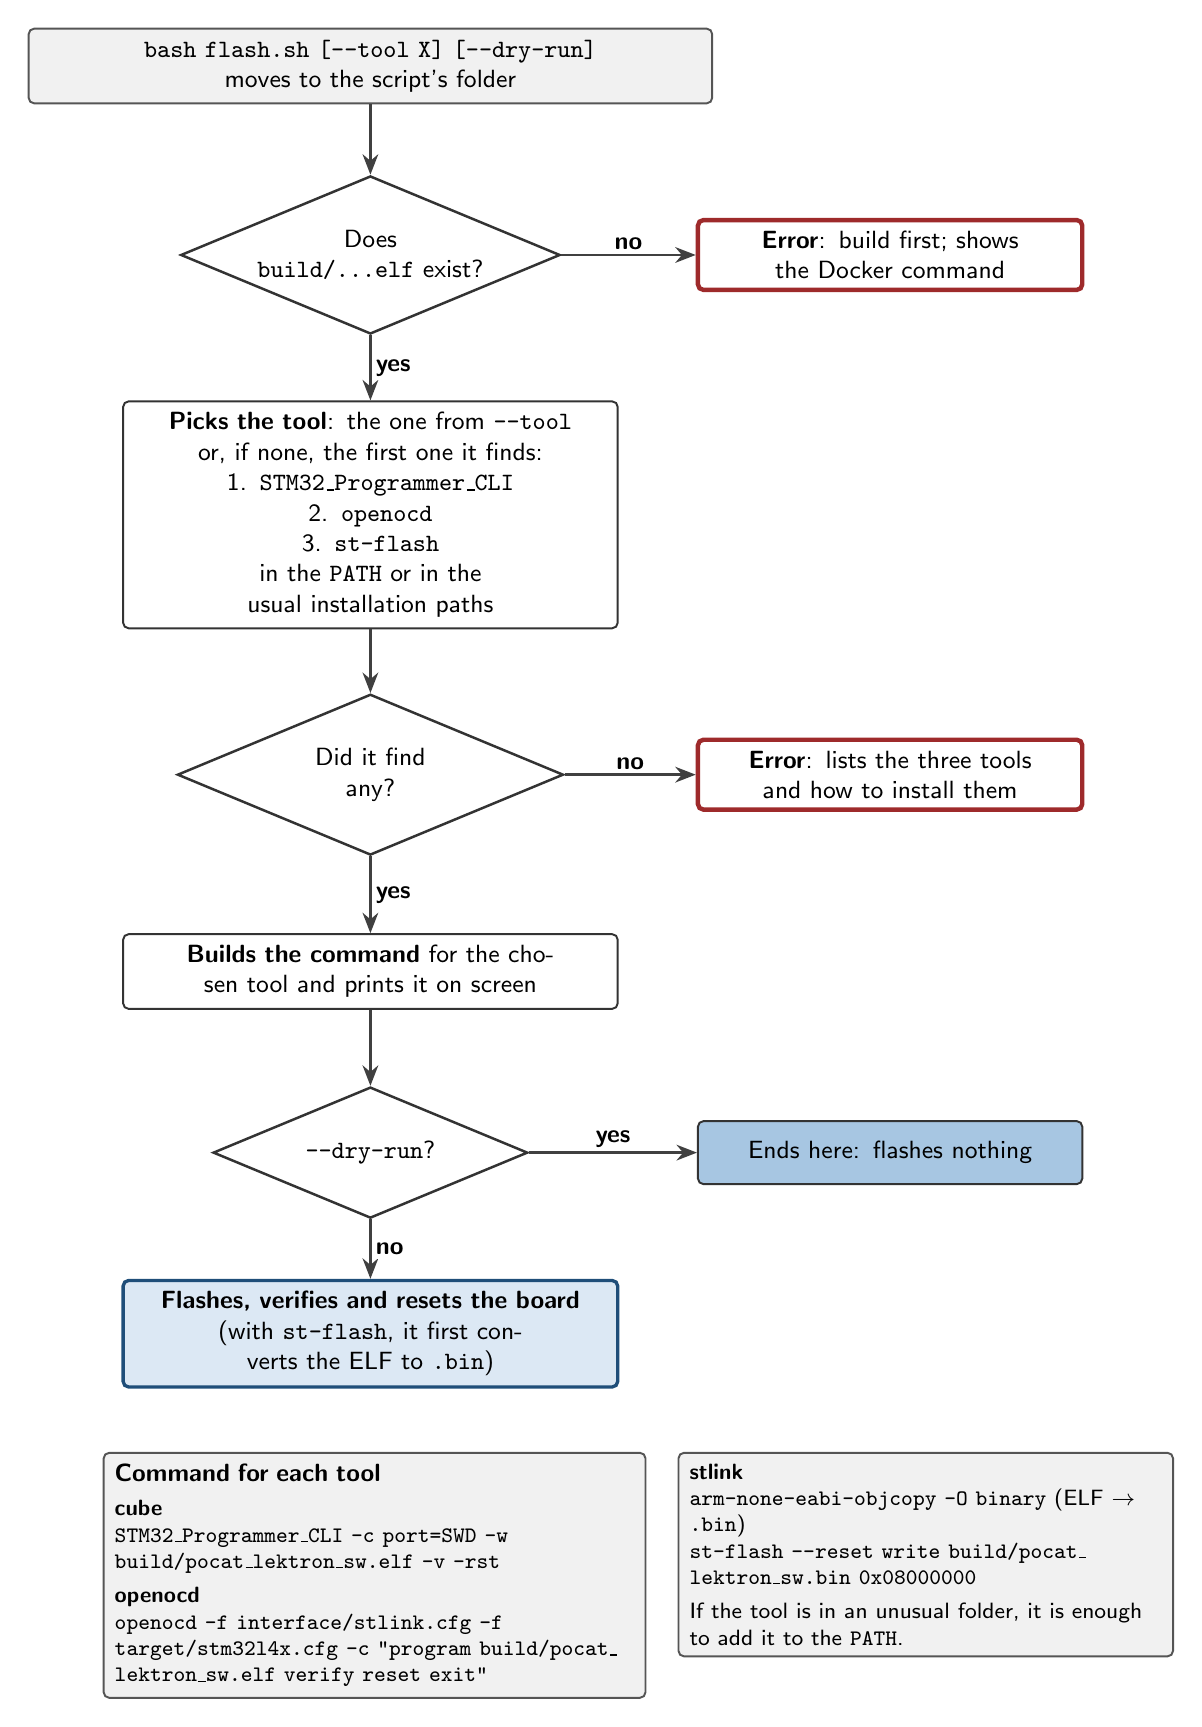
\begin{tikzpicture}[
  act/.style={box, fill=white, draw=black!80, text width=6.0cm, font=\sffamily\small},
  okn/.style={box, fill=cCovPart, draw=black!80, text width=4.6cm, font=\sffamily\small},
  bad/.style={box, fill=white, draw=cWarn, line width=1.6pt, text width=4.6cm, font=\sffamily\small},
  ]
\node[act, fill=cBg, draw=cGrey, text width=8.4cm] (s) at (0,0) {\textbf{\cd{bash flash.sh [--tool X] [--dry-run]}}\\moves to the script's folder};
\node[decision] (d0) at (0,-2.4) {Does\\\cd{build/...elf} exist?};
\node[bad] (e0) at (6.6,-2.4) {\textbf{Error}: build first; shows the Docker command};
\node[act] (pick) at (0,-5.7) {\textbf{Picks the tool}: the one from \cd{--tool} or, if none, the first one it finds:\\
  1. \cd{STM32\_Programmer\_CLI}\\ 2. \cd{openocd}\\ 3. \cd{st-flash}\\
  in the \cd{PATH} or in the usual installation paths};
\node[decision] (d1) at (0,-9.0) {Did it find\\any?};
\node[bad] (e1) at (6.6,-9.0) {\textbf{Error}: lists the three tools and how to install them};
\node[act] (cmd) at (0,-11.5) {\textbf{Builds the command} for the chosen tool and prints it on screen};
\node[decision] (d2) at (0,-13.8) {\cd{--dry-run}?};
\node[okn] (dry) at (6.6,-13.8) {Ends here: flashes nothing};
\node[act, fill=cProdL, draw=cProdD, line width=1.2pt] (run) at (0,-16.1) {\textbf{Flashes, verifies and resets the board}\\(with \cd{st-flash}, it first converts the ELF to \cd{.bin})};

\draw[arr] (s) -- (d0);
\draw[arr] (d0) -- node[lbl, above] {no} (e0);
\draw[arr] (d0) -- node[lbl, right] {yes} (pick);
\draw[arr] (pick) -- (d1);
\draw[arr] (d1) -- node[lbl, above] {no} (e1);
\draw[arr] (d1) -- node[lbl, right] {yes} (cmd);
\draw[arr] (cmd) -- (d2);
\draw[arr] (d2) -- node[lbl, above] {yes} (dry);
\draw[arr] (d2) -- node[lbl, right] {no} (run);

\node[box, fill=cBg, draw=cGrey, align=left, text width=6.6cm, font=\sffamily\footnotesize, anchor=north west] at (-3.4,-17.6)
  {\textbf{\small Command for each tool}\\[3pt]
   \textbf{cube}\\\cd{STM32\_Programmer\_CLI -c port=SWD -w build/pocat\_lektron\_sw.elf -v -rst}\\[3pt]
   \textbf{openocd}\\\cd{openocd -f interface/stlink.cfg -f target/stm32l4x.cfg -c "program build/pocat\_lektron\_sw.elf verify reset exit"}};
\node[box, fill=cBg, draw=cGrey, align=left, text width=6.0cm, font=\sffamily\footnotesize, anchor=north west] at (3.9,-17.6)
  {\textbf{stlink}\\\cd{arm-none-eabi-objcopy -O binary} (ELF \fl{} \cd{.bin})\\\cd{st-flash --reset write build/pocat\_lektron\_sw.bin 0x08000000}\\[3pt]
   If the tool is in an unusual folder, it is enough to add it to the \cd{PATH}.};
\end{tikzpicture}
\caption{How \cd{flash.sh} decides what to do. \textbf{What to take away:} the script does not know where anything is in
advance; it finds out on each PC. If it finds no tool it does not fail silently: it says which ones exist and how to
install them. \cd{--dry-run} lets you see what it would do without touching the board.}
\label{fig:flashsh}
\end{figure}

\subsection{The VS Code tasks}

\cd{.vscode/tasks.json} is shared (it is in git) and has no paths specific to any PC. They are opened
with \emph{Terminal > Run Task...}:

\begin{table}[H]
\centering\small
\begin{tabularx}{\textwidth}{@{}>{\raggedright\arraybackslash}p{5.6cm}>{\raggedright\arraybackslash}X@{}}
\toprule
Task & What it runs\\
\midrule
\emph{PoCAT: build firmware (Docker)} & \cd{docker run --rm -v <repo>:/app pocat-build-env}. It is the default build task: \cd{Ctrl+Shift+B}.\\
\emph{PoCAT: clean build firmware (Docker)} & The same with \cd{bash build.sh --clean}.\\
\emph{PoCAT: flash Nucleo} & \cd{bash flash.sh} (on Windows, with the \cd{bash.exe} from Git Bash).\\
\emph{PoCAT: build + flash} & The two previous ones, one after the other.\\
\emph{PoCAT: run host tests (Docker)} & \cd{docker run --rm -v <repo>:/app pocat-tests}: all suites.\\
\bottomrule
\end{tabularx}
\caption{Shared VS Code tasks.}
\end{table}

\subsection{Debugging with \texorpdfstring{\cd{F5}}{F5}}

With the Cortex-Debug extension, \cd{F5} (or the green arrow in the \emph{Run and Debug} panel)
builds, flashes and runs in one go. The configuration is in \cd{.vscode/launch.json}, which
is \textbf{local}: it contains the toolchain and OpenOCD paths of each PC, which is why it is not in
git. On the reference PC there are two configurations:
\begin{itemize}
\item \textbf{\emph{PoCAT: build, flash and run}}: first runs the build task
  (\cd{preLaunchTask}), flashes, and leaves the program running.
\item \textbf{\emph{Debug STM32 Nucleo L476}}: does not build; it flashes and stops at the entry of
  \cd{main()} so you can go step by step.
\end{itemize}

Under the hood, VS Code starts OpenOCD (which talks to the ST-LINK) and \cd{arm-none-eabi-gdb} (which
talks to OpenOCD), loads the ELF and controls the processor over SWD.

\textbf{The \cd{/app} problem.} The ELF is built inside the container, where the repository is at
\cd{/app}. So the debug information says the source code is at
\cd{/app/src/core/main.c}, a path that does not exist on the PC, and the debugger stops correctly but
cannot show the file:
\begin{lstlisting}[style=out]
Temporary breakpoint 1, main () at /app/src/core/main.c:45
45    /app/src/core/main.c: No such file or directory.
\end{lstlisting}
The fix is to tell GDB where \cd{/app} really is, with this entry in each
configuration of \cd{launch.json} (with the repository path of each PC, using \cd{/} slashes):
\begin{lstlisting}
"preLaunchCommands": [
    "set substitute-path /app \"C:/path/to/pocat-lektron-sw\""
]
\end{lstlisting}
Checked on 13/11: with this line GDB finds \cd{main.c} and shows its code.

\subsection{Seeing what the firmware does}

Figure~\ref{fig:hw} shows the connections. There is one detail that is misleading:

\avis{The log does not come out through the board's USB cable.}{\cd{log.c} writes to \cd{UART4} (pins PC10 and PC11, 115200
baud, 8N1). The virtual serial port that the ST-LINK creates on the PC (\cd{COMx}) is not connected to this UART, so
opening it shows nothing.}

To see the messages you need a 3.3\,V USB-serial adapter connected to PC10 (board TX)
and to GND, and a terminal at 115200 baud. Without an adapter, the way to know what
the code is doing is the debugger (\cd{F5}).

Two behaviors that are not errors: if the SX1262 radio is not connected, the communications
tasks may end up waiting; and if a task hangs, the watchdog (IWDG)
resets the board after about 30 seconds.

\begin{figure}[H]
\centering
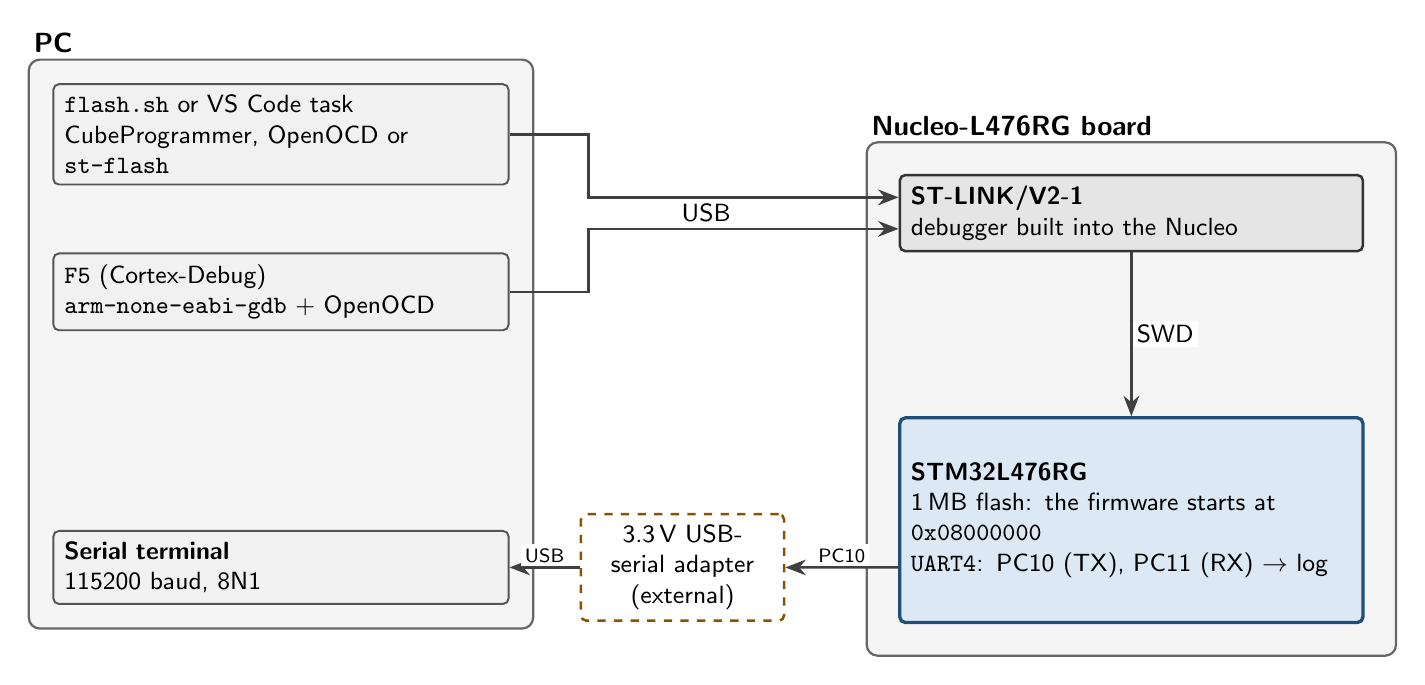
\begin{tikzpicture}[
  pc/.style={tool, text width=5.5cm, align=left, font=\sffamily\small},
  bd/.style={real, text width=5.6cm, align=left, font=\sffamily\small},
  ]
\node[pc] (p1) at (2.6,0.5) {\textbf{\cd{flash.sh}} or VS Code task\\CubeProgrammer, OpenOCD or \cd{st-flash}};
\node[pc] (p2) at (2.6,-1.5) {\textbf{\cd{F5}} (Cortex-Debug)\\\cd{arm-none-eabi-gdb} + OpenOCD};
\node[pc] (p3) at (2.6,-5.0) {\textbf{Serial terminal}\\115200 baud, 8N1};
\node[bd, fill=black!10] (st) at (13.4,-0.5) {\textbf{ST-LINK/V2-1}\\debugger built into the Nucleo};
\node[bd, fill=cProdL, draw=cProdD, line width=1.2pt, minimum height=2.6cm] (mcu) at (13.4,-4.4) {\textbf{STM32L476RG}\\
  1\,MB flash: the firmware starts at \cd{0x08000000}\\
  \cd{UART4}: PC10 (TX), PC11 (RX) \fl{} log};
\node[stub, text width=2.3cm, font=\sffamily\small] (ad) at (7.7,-5.0) {3.3\,V USB-serial adapter (external)};
\begin{scope}[on background layer]
  \node[container, fit=(st)(mcu), inner sep=4mm,
        label={[font=\sffamily\bfseries, anchor=south west, inner sep=2pt]north west:Nucleo-L476RG board}] (board) {};
  \node[container, fit=(p1)(p2)(p3), inner sep=3mm,
        label={[font=\sffamily\bfseries, anchor=south west, inner sep=2pt]north west:PC}] (pcb) {};
\end{scope}
\draw[arr] (p1.east) -- ++(1.0,0) |- ([yshift=2mm]st.west);
\draw[arr] (p2.east) -- ++(1.0,0) |- ([yshift=-2mm]st.west);
\node[lbl, font=\sffamily\small] at (8.0,-0.5) {USB};
\draw[arr] (st) -- node[lbl, right, font=\sffamily\small] {SWD} (mcu);
\draw[arr] ([yshift=-6mm]mcu.west) -- node[lbl, above, font=\sffamily\scriptsize] {PC10} (ad.east);
\draw[arr] (ad.west) -- node[lbl, above, font=\sffamily\scriptsize] {USB} (p3.east);
\end{tikzpicture}
\caption{Connections between the PC and the board. \textbf{What to take away:} flashing and debugging go through the ST-LINK
(USB and SWD), which already comes with the Nucleo. The text log goes another way, through \cd{UART4}, and needs an
external adapter.}
\label{fig:hw}
\end{figure}

\clearpage
% =====================================================================
\section{Workflow 3: running the tests}\label{sec:runtests}

\textbf{Requirements.} Docker Desktop open and the \cd{pocat-tests} image built. No board
or any other tool is needed.

\textbf{The base command}, from the root of the repository:
\begin{lstlisting}
docker run --rm -v "${PWD}:/app" pocat-tests
\end{lstlisting}
Whatever you add after it chooses what is run:

\begin{table}[H]
\centering\small
\begin{tabularx}{\textwidth}{@{}>{\raggedright\arraybackslash}p{5.2cm}>{\raggedright\arraybackslash}p{6.2cm}>{\raggedright\arraybackslash}X@{}}
\toprule
Added to the base command & What it runs inside & What for\\
\midrule
\emph{(nothing)} & \cd{ctest --output-on-failure} & all suites\\
\cd{--list} & \cd{ctest -N} & list the suites\\
\cd{--label obc} & \cd{ctest --output-on-failure -L obc} & the suites with a label: \cd{obc}, \cd{obdh}, \cd{comms}, \cd{subsys}, \cd{infra}\\
\cd{state\_machine} & \cd{ctest --output-on-failure -R state\_machine} & the suites whose name contains the text (regular expression)\\
\cd{test\_state\_machine -l} & \cd{./test/test\_state\_machine -l} & list the tests of a suite\\
\cd{test\_state\_machine -f NM\_to\_SM} & \cd{./test/test\_state\_machine -f NM\_to\_SM} & only the tests that contain the text\\
\cd{test\_obc -n <name>} & the suite binary & a single test, by exact name\\
\cd{test\_obc -x <text>} & the suite binary & all tests except those that contain the text\\
\bottomrule
\end{tabularx}
\caption{Argument forms. Rule: a suite binary is run directly only if there are \emph{at least two}
arguments and the first one is the full name of a suite; in any other case, the first argument is treated as a
\cd{ctest} regular expression.}
\label{tab:args}
\end{table}

\textbf{What happens inside} (figure~\ref{fig:flow}). The first three steps are always
the same: prepare \cd{build\_test/}, configure CMake with \cd{-DBUILD\_TESTING=ON} and
build the \cd{pocat\_tests} target, which is Unity and the 15 executables. The build is
incremental: only what has changed is rebuilt. \cd{run\_tests.sh} starts with
\cd{set -e}, so if the build fails it stops and no test is run. Only
the fourth step depends on the arguments.

There are two execution levels, and they read differently:
\begin{itemize}
\item \textbf{\cd{ctest}} runs \emph{suites}. For it, each suite is a single ``test'' that
  passes or fails as a whole. It shows details only for the ones that fail.
\item \textbf{A suite binary} (Unity) runs the \emph{tests} inside it and writes one
  line per test.
\end{itemize}

% ---------------------------------------------------------------- FIGURE: execution flow
\begin{slidefig}
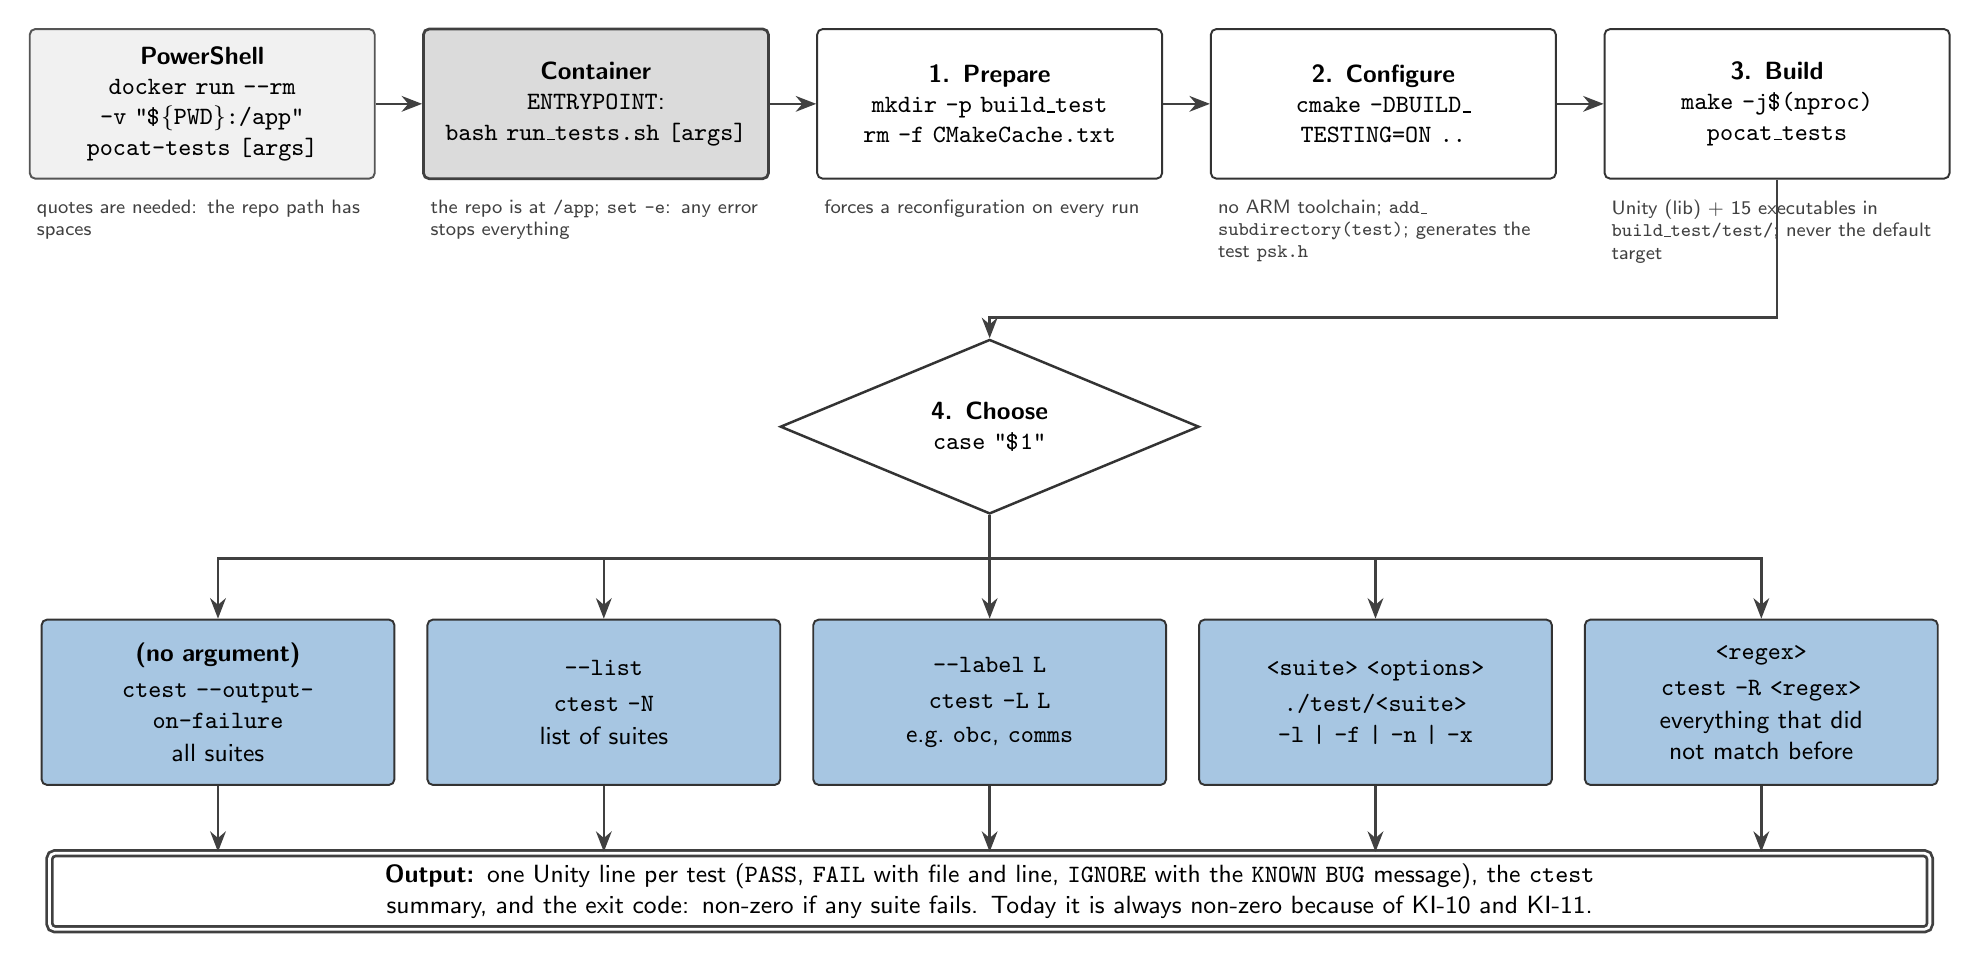
\begin{tikzpicture}[
  st/.style={box, fill=white, draw=black!80, text width=4.1cm, minimum height=1.9cm, font=\sffamily\small},
  br/.style={box, fill=cCovPart, draw=black!80, text width=4.2cm, minimum height=2.1cm, font=\sffamily\small},
  nt/.style={note, text width=4.2cm, font=\sffamily\scriptsize, anchor=north, align=left},
  ]
\def\y{10.2}
\node[tool, text width=4.1cm, minimum height=1.9cm, font=\sffamily\small] (s1) at (2.3,\y) {\textbf{PowerShell}\\\cd{docker run --rm -v "\PWD:/app" pocat-tests [args]}};
\node[img, text width=4.1cm, minimum height=1.9cm, font=\sffamily\small] (s2) at (7.3,\y) {\textbf{Container}\\\cd{ENTRYPOINT}:\\\cd{bash run\_tests.sh [args]}};
\node[st] (s3) at (12.3,\y) {\textbf{1. Prepare}\\\cd{mkdir -p build\_test}\\\cd{rm -f CMakeCache.txt}};
\node[st] (s4) at (17.3,\y) {\textbf{2. Configure}\\\cd{cmake -DBUILD\_TESTING=ON ..}};
\node[st] (s5) at (22.3,\y) {\textbf{3. Build}\\\cd{make -j\$(nproc) pocat\_tests}};
\foreach \a/\b in {s1/s2,s2/s3,s3/s4,s4/s5} \draw[arr] (\a) -- (\b);

\node[nt] at (2.3,\y-1.1) {quotes are needed: the repo path has spaces};
\node[nt] at (7.3,\y-1.1) {the repo is at \cd{/app}; \cd{set -e}: any error stops everything};
\node[nt] at (12.3,\y-1.1) {forces a reconfiguration on every run};
\node[nt] at (17.3,\y-1.1) {no ARM toolchain; \cd{add\_subdirectory(test)}; generates the test \cd{psk.h}};
\node[nt] at (22.3,\y-1.1) {Unity (lib) + 15 executables in \cd{build\_test/test/}; never the default target};

\node[decision, text width=3.8cm] (d) at (12.3,6.1) {\textbf{4. Choose}\\ \cd{case "\$1"}};
\draw[arr] (s5.south) -- ++(0,-1.75) -| (d.north);

\node[br] (b1) at (2.5,2.6) {\textbf{(no argument)}\\[2pt]\cd{ctest --output-}\\\cd{on-failure}\\[1pt]all suites};
\node[br] (b2) at (7.4,2.6) {\textbf{\cd{--list}}\\[2pt]\cd{ctest -N}\\[1pt]list of suites};
\node[br] (b3) at (12.3,2.6) {\textbf{\cd{--label L}}\\[2pt]\cd{ctest -L L}\\[1pt]e.g.\ \cd{obc}, \cd{comms}};
\node[br] (b4) at (17.2,2.6) {\textbf{\cd{<suite> <options>}}\\[2pt]\cd{./test/<suite>}\\\cd{-l | -f | -n | -x}};
\node[br] (b5) at (22.1,2.6) {\textbf{\cd{<regex>}}\\[2pt]\cd{ctest -R <regex>}\\[1pt]everything that did not match before};
\foreach \b in {b1,b2,b3,b4,b5} \draw[arr] (d.south) -- ++(0,-0.55) -| (\b.north);

\node[outp, text width=23.6cm, font=\sffamily\small] (o) at (12.3,0.2) {\textbf{Output:} one Unity line per test
  (\cd{PASS}, \cd{FAIL} with file and line, \cd{IGNORE} with the \cd{KNOWN BUG} message), the \cd{ctest} summary, and the exit code:
  non-zero if any suite fails. Today it is always non-zero because of KI-10 and KI-11.};
\foreach \b in {b1,b2,b3,b4,b5} \draw[arr] (\b.south) -- (\b.south |- o.north);
\end{tikzpicture}
\caption{What happens between \cd{docker run} and the result. \textbf{What to take away:} steps 1 to 3 are
always the same and build all the suites; only step 4 depends on the arguments. To run only a few
tests of a suite you must give the full suite name and an option (\cd{-l}, \cd{-f}, \cd{-n},
\cd{-x}); with a single argument, it is treated as a regular expression.}
\label{fig:flow}
\end{slidefig}

\subsection{Reading the output}

\textbf{One suite, test by test.} Real output of
\cd{... pocat-tests test\_state\_machine -f test\_} (after the build lines):
\begin{lstlisting}[style=out]
/app/test/suites/test_state_machine.c:396:test_freq_for_state_mapping:PASS
/app/test/suites/test_state_machine.c:397:test_boot_NM_runs_all_tasks:PASS
/app/test/suites/test_state_machine.c:400:test_NM_to_SM_switches_clock_to_2MHz_once:PASS
[...]
/app/test/suites/test_state_machine.c:353:test_transition_preserves_previous_state:IGNORE: KNOWN BUG KB-3: change_state() writes 4 bytes at PREVIOUS_STATE_ADDR, overwritten by the CURRENT_STATE write
/app/test/suites/test_state_machine.c:375:test_transition_does_not_touch_deployment_flags:IGNORE: KNOWN BUG KB-3: overlapping 4-byte state writes zero the deployment flags

-----------------------
12 Tests 0 Failures 2 Ignored
OK
\end{lstlisting}
Each line is \cd{file:line:test\_name:result}. There are three possible results:
\begin{itemize}
\item \cd{PASS}: all the assertions in the test were met.
\item \cd{FAIL}: an assertion was not met. The line says where and what was expected
  (\cd{Expected 0 Was 2}).
\item \cd{IGNORE}: the test reproduces a known error in the flight code and is parked with
  a \cd{KNOWN BUG} message (section~\ref{sec:ki}). It does not count as a failure.
\end{itemize}
The last line is \cd{OK} if there is no \cd{FAIL}, even if there are \cd{IGNORE}s.

\textbf{All suites.} Real output of the full run of 13/11/2026 (trimmed):
\begin{lstlisting}[style=out]
      Start  1: test_ht_handling
 1/15 Test  #1: test_ht_handling .................***Failed    0.04 sec
/app/test/suites/test_ht_handling.c:174:test_init_seq_counter_wrap:FAIL: Expected 0 Was 2:Oldest should be 0xFFFFFFFD at slot 0
/app/test/suites/test_ht_handling.c:330:test_bad_sector_deadlock:FAIL: Expected 16 Was 0:CRITICAL BUG: Queue deadlocked on bad sector!
14 Tests 2 Failures 0 Ignored
FAIL
      Start  2: test_notifications
 2/15 Test  #2: test_notifications ...............   Passed    0.03 sec
[...]
15/15 Test #15: test_ht_compression ..............   Passed    0.06 sec

93% tests passed, 1 tests failed out of 15

Label Time Summary:
comms     =   0.39 sec*proc (8 tests)
infra     =   0.03 sec*proc (1 test)
obc       =   0.13 sec*proc (4 tests)
obdh      =   0.04 sec*proc (1 test)
subsys    =   0.06 sec*proc (1 test)

Total Test time (real) =   0.94 sec

The following tests FAILED:
          1 - test_ht_handling (Failed)
\end{lstlisting}
How to read it:
\begin{itemize}
\item ``15 tests'' means 15 \emph{suites}. Inside them there are 253 tests.
\item For the suites that pass, only one line is shown. For the one that fails, \cd{ctest}
  shows the whole Unity output; here only the two \cd{FAIL} lines have been kept.
\item The two failures are the expected ones: KI-10 and KI-11. \textbf{Any other \cd{FAIL}
  line, or any other suite in red, is a real regression.}
\item All of it takes less than a second. What takes time is the build, the first time.
\end{itemize}

\textbf{The exit code.} It is 0 only if all suites pass. As long as KI-10 and KI-11
fail on purpose, a full run always returns a non-zero value (in PowerShell
you can see it with \cd{\$LASTEXITCODE}). This prevents using it as is in continuous
integration; it is one of the pending decisions (section~\ref{sec:roadmap}).

\begin{table}[H]
\centering\small
\begin{tabularx}{\textwidth}{@{}>{\raggedright\arraybackslash}p{5.4cm}>{\raggedright\arraybackslash}X@{}}
\toprule
What you see & What it means\\
\midrule
A build error and no test run & The production code or a suite does not compile with native gcc. \cd{set -e} stops the script before running anything.\\
\cd{fake\_rtos: deadlock in xQueueReceive} (or another API) & The code made an infinite wait (\cd{portMAX\_DELAY}) that nobody can satisfy. On the satellite, that task would hang (section~\ref{sec:rtos}).\\
\cd{configASSERT} with file and line & The code called FreeRTOS with arguments that the real kernel would reject.\\
An \cd{AddressSanitizer} report or a UBSan \cd{runtime error:} & The code read or wrote outside a buffer, or did an undefined operation (overflow, division by zero). The suite aborts.\\
\cd{***Timeout} in \cd{ctest} & The suite exceeded 60\,s (\cd{POCAT\_TEST\_TIMEOUT}). Since a suite takes hundredths of a second, the code under test is stuck in a loop.\\
\cd{unbalanced critical section} / \cd{unbalanced scheduler suspend} & The code entered a critical section, or suspended the scheduler, and did not leave it. The \cd{tearDown()} of each suite checks this.\\
\bottomrule
\end{tabularx}
\caption{Failures that are not a normal assertion, and what they mean.}
\label{tab:testerrors}
\end{table}

\textbf{From Git Bash} you must stop MSYS from rewriting paths:
\cd{MSYS\_NO\_PATHCONV=1 docker run --rm -v "\$(pwd -W)":/app pocat-tests}.

\textbf{The telecommand catalog.} \cd{test\_tc\_handler} has one test for each telecommand
and can be used as a list of ``what the satellite does when it receives X'':
\begin{lstlisting}
docker run --rm -v "${PWD}:/app" pocat-tests test_tc_handler -l                # the whole catalog
docker run --rm -v "${PWD}:/app" pocat-tests test_tc_handler -f TC_REQUEST_HK  # one telecommand
docker run --rm -v "${PWD}:/app" pocat-tests test_tc_handler -f LORA           # all the LoRa cases
\end{lstlisting}

\clearpage
% =====================================================================
\section{Workflow 4: day-to-day work}\label{sec:daily}

Figure~\ref{fig:loop} is the full cycle of a change, from editing to the commit. The
host tests are the fast step in the middle: in seconds they tell you whether the logic is still right, before
spending time on the board.

\begin{figure}[H]
\centering
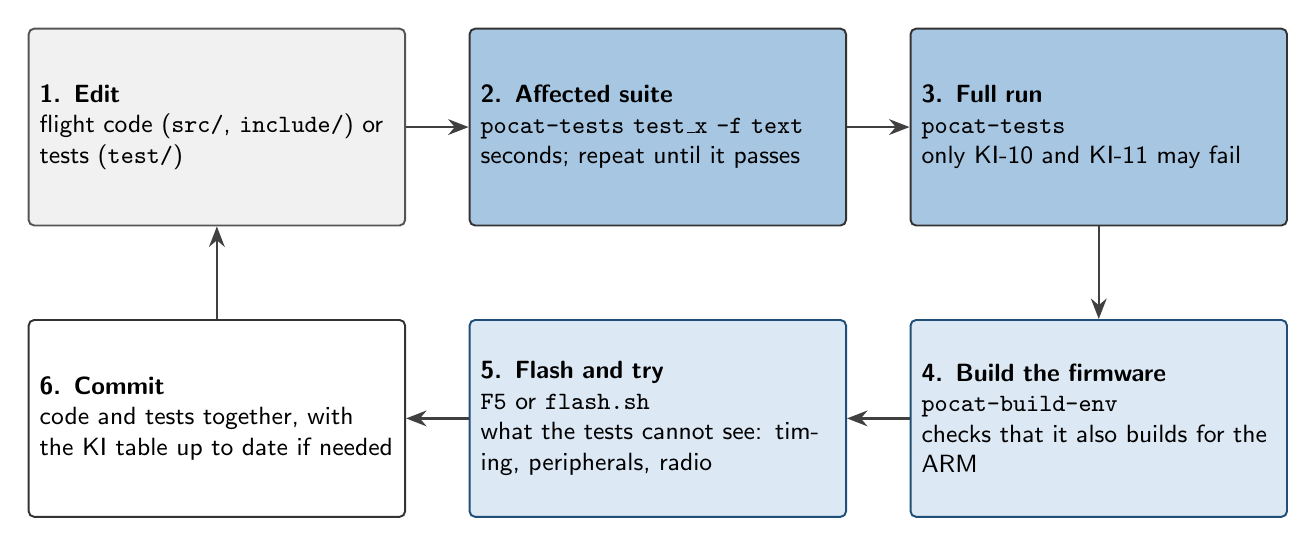
\begin{tikzpicture}[
  stp/.style={box, fill=white, draw=black!80, text width=4.5cm, minimum height=2.5cm, align=left, font=\sffamily\small},
  ]
\node[stp, fill=cBg, draw=cGrey] (a) at (0,0) {\textbf{1. Edit}\\flight code (\cd{src/}, \cd{include/}) or tests (\cd{test/})};
\node[stp, fill=cCovPart] (b) at (5.6,0) {\textbf{2. Affected suite}\\\cd{pocat-tests test\_x -f text}\\seconds; repeat until it passes};
\node[stp, fill=cCovPart] (c) at (11.2,0) {\textbf{3. Full run}\\\cd{pocat-tests}\\only KI-10 and KI-11 may fail};
\node[stp, fill=cProdL, draw=cProdD] (d) at (11.2,-3.7) {\textbf{4. Build the firmware}\\\cd{pocat-build-env}\\checks that it also builds for the ARM};
\node[stp, fill=cProdL, draw=cProdD] (e) at (5.6,-3.7) {\textbf{5. Flash and try}\\\cd{F5} or \cd{flash.sh}\\what the tests cannot see: timing, peripherals, radio};
\node[stp] (f) at (0,-3.7) {\textbf{6. Commit}\\code and tests together, with the KI table up to date if needed};
\draw[arr] (a) -- (b); \draw[arr] (b) -- (c); \draw[arr] (c) -- (d);
\draw[arr] (d) -- (e); \draw[arr] (e) -- (f); \draw[arr] (f) -- (a);
\end{tikzpicture}
\caption{The cycle of a change. Light blue: host tests (fast, no board). Very light blue with a dark
border: firmware and board. \textbf{What to take away:} steps 2 and 3 take seconds and catch logic
errors; steps 4 and 5 are still necessary, because a host test says nothing about real timing,
priorities, stacks or peripherals.}
\label{fig:loop}
\end{figure}

\subsection{Recipes}

\textbf{I changed flight code.} Run the module's suite (table~\ref{tab:suites}) and
then all of them. If a test fails, there are two possibilities: the change broke a
behavior (fix the code) or the behavior changed on purpose (update the
test and its documentation). If you fixed a known problem, delete the
\cd{TEST\_IGNORE\_MESSAGE} line from its test and update the row in \cd{test/README.md}.

\textbf{I want to add a test to a suite that already exists.}
\begin{enumerate}
\item Write the function \cd{void test\_<action>\_<expected\_result>(void)} with its
  Doxygen block (\cd{@brief}: what must happen; \cd{@details}: the scenario and why it matters for the satellite).
\item Add \cd{POCAT\_RUN\_TEST(test\_...);} to the \cd{main()} at the end of the file. If it is
  forgotten, the test compiles but never runs.
\item Run it alone: \cd{... pocat-tests test\_<suite> -f <part\_of\_the\_name>}.
\end{enumerate}

\textbf{I want to test a module that has no suite.}
\begin{enumerate}
\item Create \cd{test/suites/test\_<name>.c} by copying a similar suite
  (\cd{test\_task\_management.c} is the reference example). The minimal structure is:
\begin{lstlisting}[language=C]
#include "unity.h"
#include "pocat_test_main.h"
#include "fake_rtos.h"
#include "<module>.c"             /* R1: the .c under test, included */

void setUp(void) {                /* R2: everything clean before each test */
    fake_rtos_reset();
    /* reset of the other fakes and of the statics in <module>.c */
}
void tearDown(void) {             /* R3: balanced critical sections */
    TEST_ASSERT_EQUAL_INT(0, fake_rtos_critical_depth());
    TEST_ASSERT_EQUAL_INT(0, fake_rtos_suspend_all_depth());
}

/** @brief Expected behavior. @details Scenario and why it matters. */
void test_<action>_<expected_result>(void) { /* ... */ }

int main(int argc, char **argv) { /* R6 */
    if (pocat_parse_args(argc, argv) != 0) return 1;
    POCAT_BEGIN();
    POCAT_RUN_TEST(test_<action>_<expected_result>);
    return POCAT_END();
}
\end{lstlisting}
\item Register it with one line in \cd{test/CMakeLists.txt}:
\begin{lstlisting}
pocat_add_suite(test_<name> LABEL <obc|obdh|comms|subsys|infra>
  SOURCES ${SRC_DIR}/utils/notifications.c mocks/fake_obdh_requests.c)
\end{lstlisting}
  Options: \cd{NO\_FAKES} (does not link \cd{fake\_rtos} or \cd{fake\_hal}), \cd{NO\_SANITIZE} (needs a
  comment that justifies it) and \cd{INCLUDES <dirs>} (directories that are searched first).
  \cd{run\_tests.sh} must not be touched.
\item Run it alone and then the full run. Add it to the suite table in \cd{test/README.md}.
\end{enumerate}

\textbf{I am adding a new telecommand} (in \cd{include/subsystems/comms/types.h}):
\begin{enumerate}
\item add the \cd{case} to \cd{tc\_process()};
\item add the identifier to the \cd{known[]} list of the test
  \cd{test\_every\_tc\_id\_is\_either\_handled\_or\_nacked}. This list is a hand-made copy
  of the catalog: the test catches a \cd{case} with no entry in \cd{known[]} and the other way round,
  but not an identifier forgotten in both places;
\item write a test \cd{test\_TC\_<NAME>\_<effect>}.
\end{enumerate}

\textbf{While writing a test I found an error in the flight code.} Do not fix it from the
test work: follow the \cd{KNOWN BUG} procedure in section~\ref{sec:ki}.

\subsection{The six rules (R1--R6)}

They are in \cd{test/README.md} and all the suites follow them.

\begin{table}[H]
\centering\small
\begin{tabularx}{\textwidth}{@{}l>{\raggedright\arraybackslash}p{4.2cm}>{\raggedright\arraybackslash}X@{}}
\toprule
 & Rule & Why\\
\midrule
R1 & The \cd{.c} under test is included with \cd{\#include}; files without state go in \cd{SOURCES}. Never both for the same file. &
By including it, the test sees the module's \cd{static} variables and functions. Doing both at once gives duplicate symbols.\\
R2 & \cd{setUp()} resets everything: the fakes and the \cd{static}s of the included modules. &
Without this, a test inherits the state of the previous one and the result depends on the order.\\
R3 & \cd{tearDown()} checks that the depth of critical sections and of scheduler suspension is back to 0. &
A critical section left open would freeze the satellite.\\
R4 & A known production error is a test with \cd{TEST\_IGNORE\_MESSAGE("KNOWN BUG ...")} on the first line, and a row in the table. &
The error stays visible and documented, but it does not break the run. Fixing it means deleting one line.\\
R5 & Doxygen documentation everywhere and names that read like a sentence: \cd{test\_<action>\_<result>}. &
The name and the \cd{@brief} must say what the satellite does without having to read the test code.\\
R6 & \cd{main()} is the one from the template in \cd{pocat\_test\_main.h}. &
It gives all the suites the options \cd{-l}, \cd{-f}, \cd{-n} and \cd{-x}.\\
\bottomrule
\end{tabularx}
\caption{Suite conventions.}
\label{tab:rules}
\end{table}

\textbf{Typical mistakes when writing tests.}
\begin{itemize}
\item Forgetting the \cd{POCAT\_RUN\_TEST} in \cd{main()}: the test does not run and nobody notices.
\item Forgetting to reset a \cd{static} in \cd{setUp()}: tests that pass alone and fail together.
\item Including \cd{lora\_cfg.c} without \cd{INCLUDES \$\{CMAKE\_SOURCE\_DIR\}/external/RadioLib/src}: it cannot find \cd{TypeDef.h}.
\item Assuming that \cd{fake\_obdh\_requests} validates flash alignment: it does not (section~\ref{sec:fakes}).
\item Checking only what the fake itself wrote: the test always passes and proves nothing.
\end{itemize}
% =====================================================================
\part{How the tests work inside}

\section{The central idea: the same code, a different environment}\label{sec:idea}

A host test does not test a copy or a simulation of the firmware. It compiles \emph{the same
\cd{.c} file} that goes to the STM32. What changes is what lies underneath
(figure~\ref{fig:stack}). Three mechanisms make this possible:

\begin{enumerate}
\item \textbf{The suite does \cd{\#include} of the production \cd{.c}.} For example,
  \cd{test\_obc.c} contains \cd{\#include "obc.c"}, \cd{"state\_machine.c"},
  \cd{"task\_management.c"} and \cd{"health.c"}. This way the test and the flight code
  are compiled as a single file, and the test sees the \cd{static} variables and functions of
  the module: it can inspect and reset them. Files without state (\cd{notifications.c},
  \cd{frame.c}...) are linked separately, with \cd{SOURCES}.
\item \textbf{Test headers that shadow the real ones.} The include path puts
  \cd{test/mocks/stubs\_rtos/} first (\cd{FreeRTOS.h}, \cd{task.h}, \cd{queue.h}, \cd{semphr.h},
  \cd{event\_groups.h}, \cd{timers.h}) and \cd{test/mocks/stubs\_hal/} (\cd{stm32l4xx\_hal.h},
  \cd{stm32l476xx.h}). When the flight code does \cd{\#include "FreeRTOS.h"}, it gets the test
  version, which only declares types and prototypes.
\item \textbf{Fakes that implement those prototypes.} \cd{fake\_rtos.c} implements
  \cd{xTaskCreate}, \cd{xQueueSend}, \cd{xTaskNotify}...; \cd{fake\_hal.c} defines the
  peripheral handles; \cd{fake\_obdh\_requests.c} implements \cd{obdh\_write\_request}
  on top of a flash image in RAM; and so on for the rest.
\end{enumerate}

The flight code is not modified in any way to make it testable: there is no \cd{\#ifdef TEST}.

\textbf{Names.} \cd{fake\_*} is a simplified implementation that works and that the test
can control and inspect. \cd{stub\_*} does nothing; it is only there so that linking works.
\cd{mock\_*} are the files of the first suite (\cd{test\_ht\_handling}), which have
kept their name.

% ---------------------------------------------------------------- FIGURE: stack (draw.io)
\begin{slidefig}
\drawio[\linewidth]{test-layers}
\caption{Layer substitution (draw.io: \cd{figures/test-layers.drawio}). \textbf{What to take away:} the two blue rows are the same on both
sides, that is, the code under test is exactly the code that flies. Everything below it (operating
system, HAL, flash, radio) is swapped for test parts that run on the PC and that the test can
control and inspect.}
\label{fig:stack}
\end{slidefig}

\subsection{How a suite is built: \texorpdfstring{\cd{pocat\_add\_suite()}}{pocat\_add\_suite()}}

Each suite is an independent executable. In \cd{test/CMakeLists.txt}, one line
registers it; for example:
\begin{lstlisting}
pocat_add_suite(test_state_machine LABEL obc
  SOURCES ${SRC_DIR}/utils/notifications.c mocks/stub_task_entries.c support/sim_tasks.c
          mocks/fake_clock.c mocks/fake_obdh_requests.c)
\end{lstlisting}
With this, the \cd{pocat\_add\_suite()} function does six things:
\begin{enumerate}
\item It creates the \cd{test\_state\_machine} executable from \cd{suites/test\_state\_machine.c}, the
  files in \cd{SOURCES} and, automatically, \cd{fake\_rtos.c} and \cd{fake\_hal.c} (unless
  \cd{NO\_FAKES} is passed; only \cd{test\_ht\_handling} does this).
\item It sets the include path, in this order: (a) the suite's own \cd{INCLUDES}; (b) the
  generated test \cd{psk.h}; (c) \cd{test/support}, \cd{test/mocks},
  \cd{stubs\_hal} and \cd{stubs\_rtos}; (d) the real project headers; (e) the
  \cd{src/} directories, so that the suite can do \cd{\#include "x.c"}. This order is what
  makes the stubs win over the real headers.
\item It links the executable with Unity and compiles it with \cd{-Wall -Wextra -g -O0}.
\item It enables the \emph{sanitizers}: \cd{-fsanitize=address,undefined}
  \cd{-fno-sanitize-recover=undefined}.
\item It registers the executable in \cd{ctest} with a 60\,s limit and the \cd{LABEL} label.
\item It makes the executable a dependency of the \cd{pocat\_tests} target, which is what \cd{run\_tests.sh} builds.
  This is why adding a suite does not require touching the script.
\end{enumerate}

\textbf{What the \emph{sanitizers} give you.} AddressSanitizer and UBSan are checks that
the compiler adds to the program. If the flight code reads or writes outside a buffer,
uses freed memory, overflows a signed integer or divides by zero, the suite
aborts with a report that gives the file and the line. On the STM32 these errors corrupt
memory silently; here they are visible. KI-20 (a modulo by zero in \cd{arq.c}) was confirmed
this way.

\textbf{The test PSK.} The CMake in \cd{test/} generates its own \cd{psk.h} inside
\cd{build\_test/}, with the key \cd{00 01 02 ... 0F}. Because it comes first in the include
path, it wins over any development \cd{psk.h}. The frames in the comms tests are
really signed and verified with this key, which is not the flight key.

\subsection{What happens inside a suite executable}

All suites end with the same \cd{main()}, from \cd{pocat\_test\_main.h}:
\begin{lstlisting}[language=C]
int main(int argc, char **argv) {
    if (pocat_parse_args(argc, argv) != 0) return 1;
    POCAT_BEGIN();
    POCAT_RUN_TEST(test_freq_for_state_mapping);
    POCAT_RUN_TEST(test_boot_NM_runs_all_tasks);
    /* ... one line per test ... */
    return POCAT_END();
}
\end{lstlisting}
Figure~\ref{fig:lifecycle} shows what it does. The important point is isolation: before
each test, \cd{setUp()} runs and leaves the fakes and the module's \cd{static} variables as if
the satellite had just booted. After the test, \cd{tearDown()} checks that the code did not
leave anything half done. A test cannot depend on what the previous one did.

\begin{figure}[p]
\centering
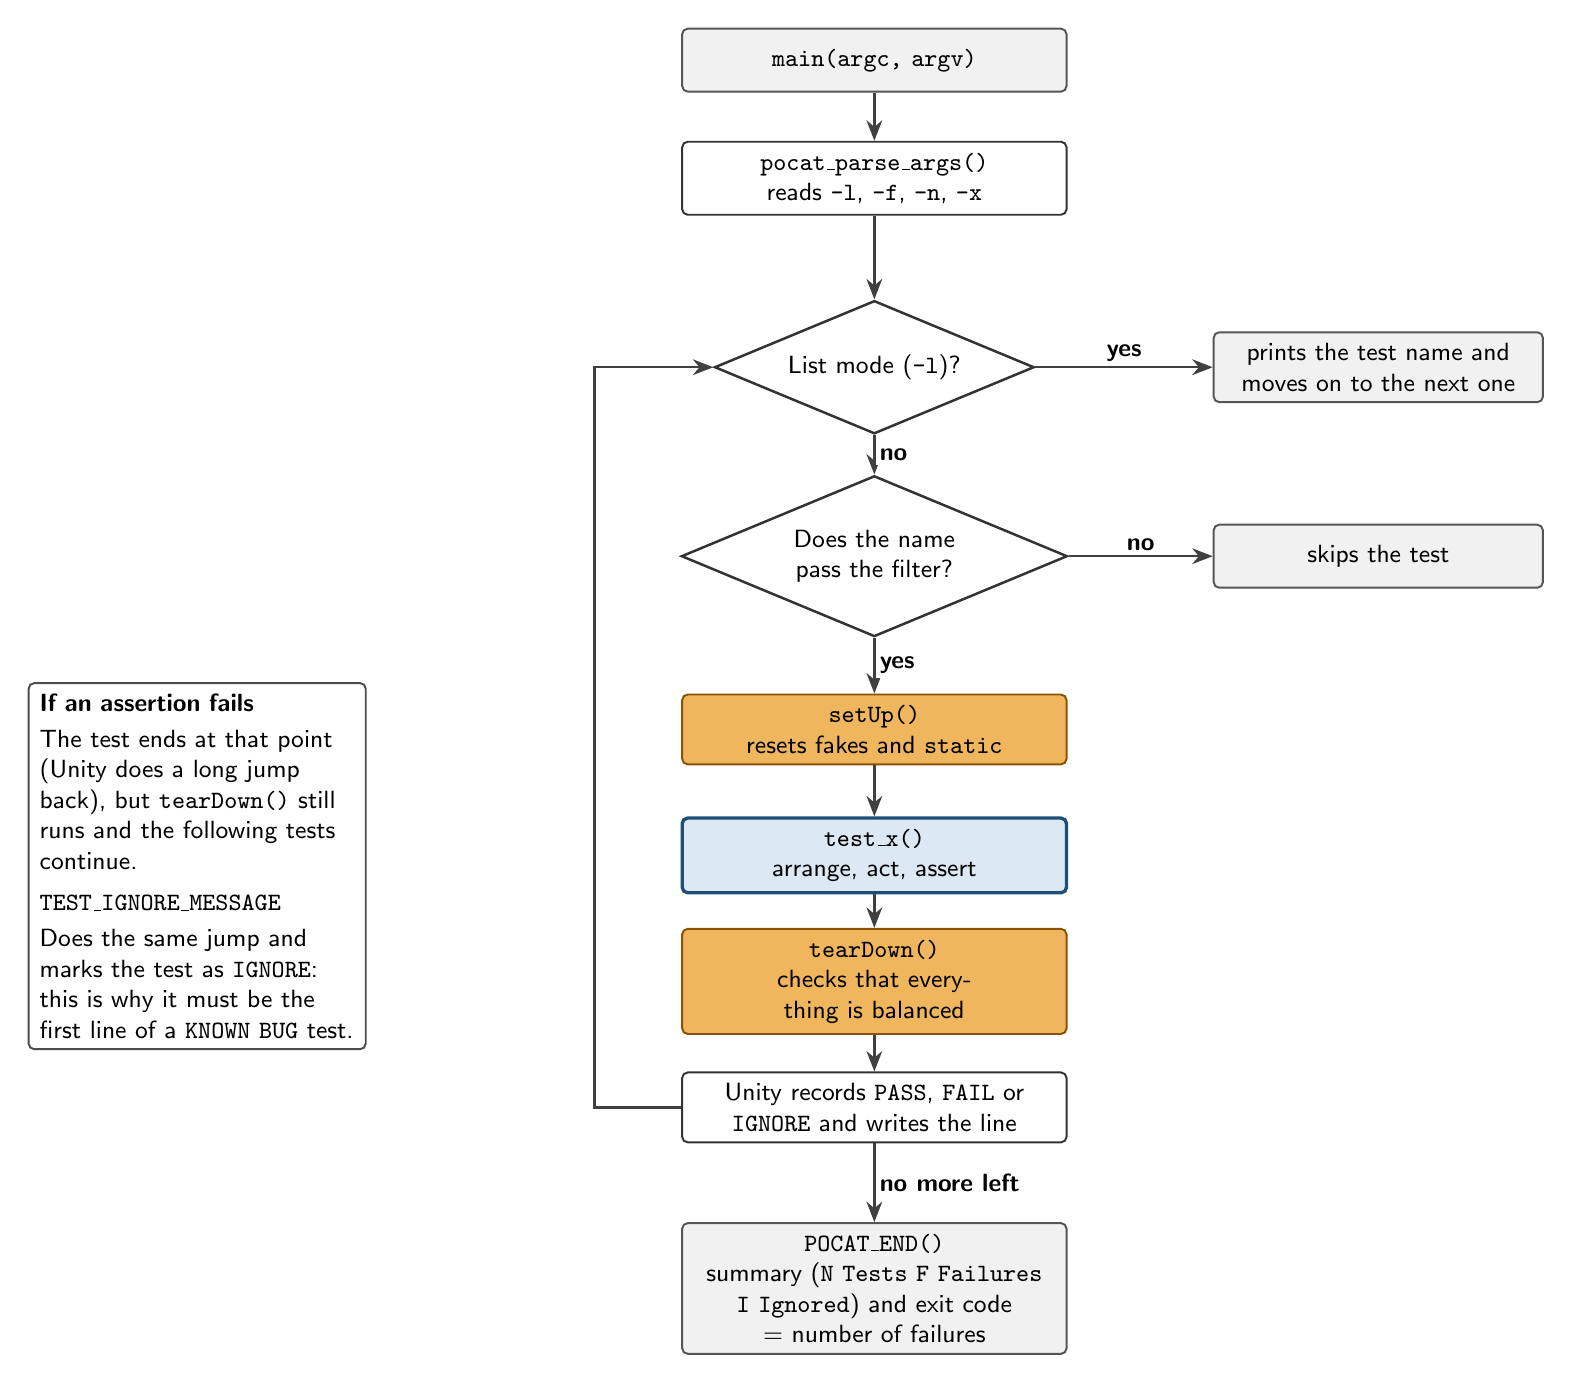
\begin{tikzpicture}[
  act/.style={box, fill=white, draw=black!80, text width=4.6cm, font=\sffamily\small},
  side/.style={box, fill=cBg, draw=cGrey, text width=3.9cm, font=\sffamily\small},
  ]
\node[act, fill=cBg, draw=cGrey] (m0) at (0,0) {\textbf{\cd{main(argc, argv)}}};
\node[act] (m1) at (0,-1.5) {\cd{pocat\_parse\_args()}\\reads \cd{-l}, \cd{-f}, \cd{-n}, \cd{-x}};
\node[decision] (d1) at (0,-3.9) {List mode (\cd{-l})?};
\node[side] (l1) at (6.4,-3.9) {prints the test name and moves on to the next one};
\node[decision] (d2) at (0,-6.3) {Does the name pass the filter?};
\node[side] (l2) at (6.4,-6.3) {skips the test};
\node[act, fill=cFakeL, draw=cFakeD] (su) at (0,-8.5) {\textbf{\cd{setUp()}}\\resets fakes and \cd{static}};
\node[act, fill=cProdL, draw=cProdD, line width=1.2pt] (te) at (0,-10.1) {\textbf{\cd{test\_x()}}\\arrange, act, assert};
\node[act, fill=cFakeL, draw=cFakeD] (td) at (0,-11.7) {\textbf{\cd{tearDown()}}\\checks that everything is balanced};
\node[act] (re) at (0,-13.3) {Unity records \cd{PASS}, \cd{FAIL} or \cd{IGNORE} and writes the line};
\node[act, fill=cBg, draw=cGrey] (en) at (0,-15.6) {\textbf{\cd{POCAT\_END()}}\\summary (\cd{N Tests F Failures I Ignored}) and exit code = number of failures};

\draw[arr] (m0) -- (m1);
\draw[arr] (m1) -- (d1);
\draw[arr] (d1) -- node[lbl, above] {yes} (l1);
\draw[arr] (d1) -- node[lbl, right] {no} (d2);
\draw[arr] (d2) -- node[lbl, above] {no} (l2);
\draw[arr] (d2) -- node[lbl, right] {yes} (su);
\draw[arr] (su) -- (te);
\draw[arr] (te) -- (td);
\draw[arr] (td) -- (re);
\draw[arr] (re.west) -- ++(-1.1,0) |- (d1.west);
\draw[arr] (re) -- node[lbl, right] {no more left} (en);

\node[box, fill=white, draw=black!70, align=left, text width=4.0cm, font=\sffamily\small, anchor=north] at (-8.6,-7.9)
  {\textbf{If an assertion fails}\\[2pt]
   The test ends at that point (Unity does a long jump back), but \cd{tearDown()} still runs and the following
   tests continue.\\[4pt]
   \textbf{\cd{TEST\_IGNORE\_MESSAGE}}\\[2pt]
   Does the same jump and marks the test as \cd{IGNORE}: this is why it must be the first line of a \cd{KNOWN BUG} test.};
\end{tikzpicture}
\caption{Life of a suite executable. Each \cd{POCAT\_RUN\_TEST(test\_x)} in \cd{main()} is one turn
of the loop. \textbf{What to take away:} each test runs between a \cd{setUp()} that leaves everything clean and a
\cd{tearDown()} that checks that the code did not leave anything open. The exit code of the executable is the
number of failed tests, and \cd{ctest} looks at it to decide whether the suite passes.}
\label{fig:lifecycle}
\end{figure}

\subsection{What a host test cannot tell you}

Nothing about real time, priorities, preemption, interrupts, stack sizes or
peripherals. Also, the PC is 64-bit and the STM32 is 32-bit: \cd{long} and \cd{size\_t} have
different sizes. A host test verifies the \emph{logic}; the board is still
needed for everything else.

\clearpage
% =====================================================================
\section{A real test, call by call}\label{sec:trace}

This section follows two real tests from start to finish, to see how all the
pieces fit together.

\subsection{A state transition: NM \texorpdfstring{\fl{}}{to} SM}

The test is in \cd{test/suites/test\_state\_machine.c}. It checks that, when going from nominal
mode to survival mode, the clock drops to 2\,MHz exactly once and with the
scheduler suspended:
\begin{lstlisting}[language=C]
void test_NM_to_SM_switches_clock_to_2MHz_once(void)
{
    obc_state_t state = OBC_STATE_NM;
    boot_in(state);                                              /* arrange */

    check_next_state(&state, N_OBC_EXIT_STATE_TO_OBC_STATE_SM);  /* act     */

    TEST_ASSERT_EQUAL_INT(OBC_STATE_SM, state);                  /* assert  */
    TEST_ASSERT_EQUAL_INT(1, fake_clock_switch_count());
    TEST_ASSERT_EQUAL_INT(CLK_FREQ_2MHZ, fake_clock_last_switch_freq());
    TEST_ASSERT_EQUAL_INT(1, fake_clock_last_switch_suspend_depth());
    TEST_ASSERT_EQUAL_INT(1, fake_clock_reconfigure_count());
    TEST_ASSERT_EQUAL_INT(CLK_FREQ_2MHZ, fake_clock_last_reconfigure_freq());
    TEST_ASSERT_EQUAL_INT(CLK_FREQ_2MHZ, clock_get_current());
}
\end{lstlisting}

It is only a few lines, but underneath the whole real path of \cd{state\_machine.c} and
\cd{task\_management.c} runs. Figure~\ref{fig:seq} draws it; the numbers are those of this
list.

\begin{enumerate}[label=\textbf{\arabic*.}]
\item \textbf{\cd{setUp()}} (before the test). It resets \cd{fake\_rtos}, \cd{fake\_hal},
  \cd{fake\_clock} (which starts at 80\,MHz), \cd{fake\_obdh\_requests} (flash at \cd{0xFF}) and
  \cd{sim\_tasks}; it zeroes the task table and the state of the health module; and it installs
  \cd{sim\_tasks\_run\_pending} as the \emph{block hook}.
\item \textbf{Boot.} \cd{boot\_in(NM)} calls \cd{state\_machine\_boot()}, which asks
  \cd{tm\_create\_tasks()} for the 7 tasks. The fake FreeRTOS records them (name, priority,
  number) but does not run any of them.
\item \textbf{The action.} \cd{check\_next\_state()} sees the ``go to SM'' bit and calls the
  private function \cd{change\_state()}.
\item \cd{change\_state()} saves the previous state with \cd{obdh\_write\_request()}. On the satellite
  this enqueues a request to the OBDH task; here, \cd{fake\_obdh\_requests} writes it
  directly to its RAM image and records it in the call log.
\item \cd{tm\_pause\_tasks()} sends \cd{N\_TASK\_PAUSE} to the 7 tasks of the old state with
  \cd{xTaskNotify}. The fake leaves each notification pending and logs it.
\item Next it waits for the 7 ACKs with \cd{xEventGroupWaitBits}. On the satellite, the OBC would
  block here and the other tasks would run. In the test there is no other thread:
  the wait cannot be satisfied.
\item Before giving up, the fake FreeRTOS calls the \emph{block hook}.
  \cd{sim\_tasks\_run\_pending()} walks through the tasks with a pending notification and, for
  each one, makes it ``current'', reads the notification with the real \cd{wait\_for\_notification()}
  and passes it to the real \cd{tm\_check\_pause()}.
\item \cd{tm\_check\_pause()} marks the task as paused, removes it from health
  monitoring and sends its ACK with \cd{xEventGroupSetBits}. When the hook finishes, all 7 ACKs are there,
  the wait is satisfied and \cd{tm\_pause\_tasks()} returns.
\item Since SM runs at 2\,MHz and the clock is at 80, \cd{change\_state()} suspends the
  scheduler (\cd{vTaskSuspendAll}; the fake records depth 1).
\item It calls \cd{clock\_switch\_to\_freq(2\,MHz)} and \cd{periph\_reconfigure\_for\_freq(2\,MHz)}.
  \cd{fake\_clock} counts the calls and records what the suspend depth was at the
  moment of the switch.
\item \cd{xTaskResumeAll()}: the depth goes back to 0.
\item \cd{tm\_resume\_tasks()} sends \cd{N\_TASK\_RESUME} to the 4 tasks of SM (EPS, COMMS,
  OBDH, TRANSCEIVER) and waits for the ACKs with the same mechanism as steps 6 to 8.
\item \cd{change\_state()} updates \cd{state} and saves it to \cd{CURRENT\_STATE\_ADDR}.
\item \textbf{The assertions.} The test asks the fakes what happened: the state is SM;
  there was exactly one clock switch, to 2\,MHz and with suspend depth 1;
  one peripheral reconfiguration; and the clock now reads 2\,MHz.
\item \textbf{\cd{tearDown()}} checks that the critical section depth and the scheduler
  suspend depth are 0.
\end{enumerate}

Two details of this example apply to all tests:
\begin{itemize}
\item \textbf{The flight code does not know it is in a test.} It makes the same calls to
  FreeRTOS, the clock and the OBDH that it would make on the board.
\item \textbf{The test does not simulate the pause protocol: it runs it.} The hook only acts as the
  ``scheduler'' and gives each task its turn; the real
  \cd{tm\_check\_pause()} decides what happens. If the protocol has a bug, the test sees it: KI-4 (a pending PAUSE and
  RESUME at the same time leave the task paused forever) is reproduced exactly this way.
\end{itemize}

% ---------------------------------------------------------------- FIGURA: seqüència
\begin{slidefig}
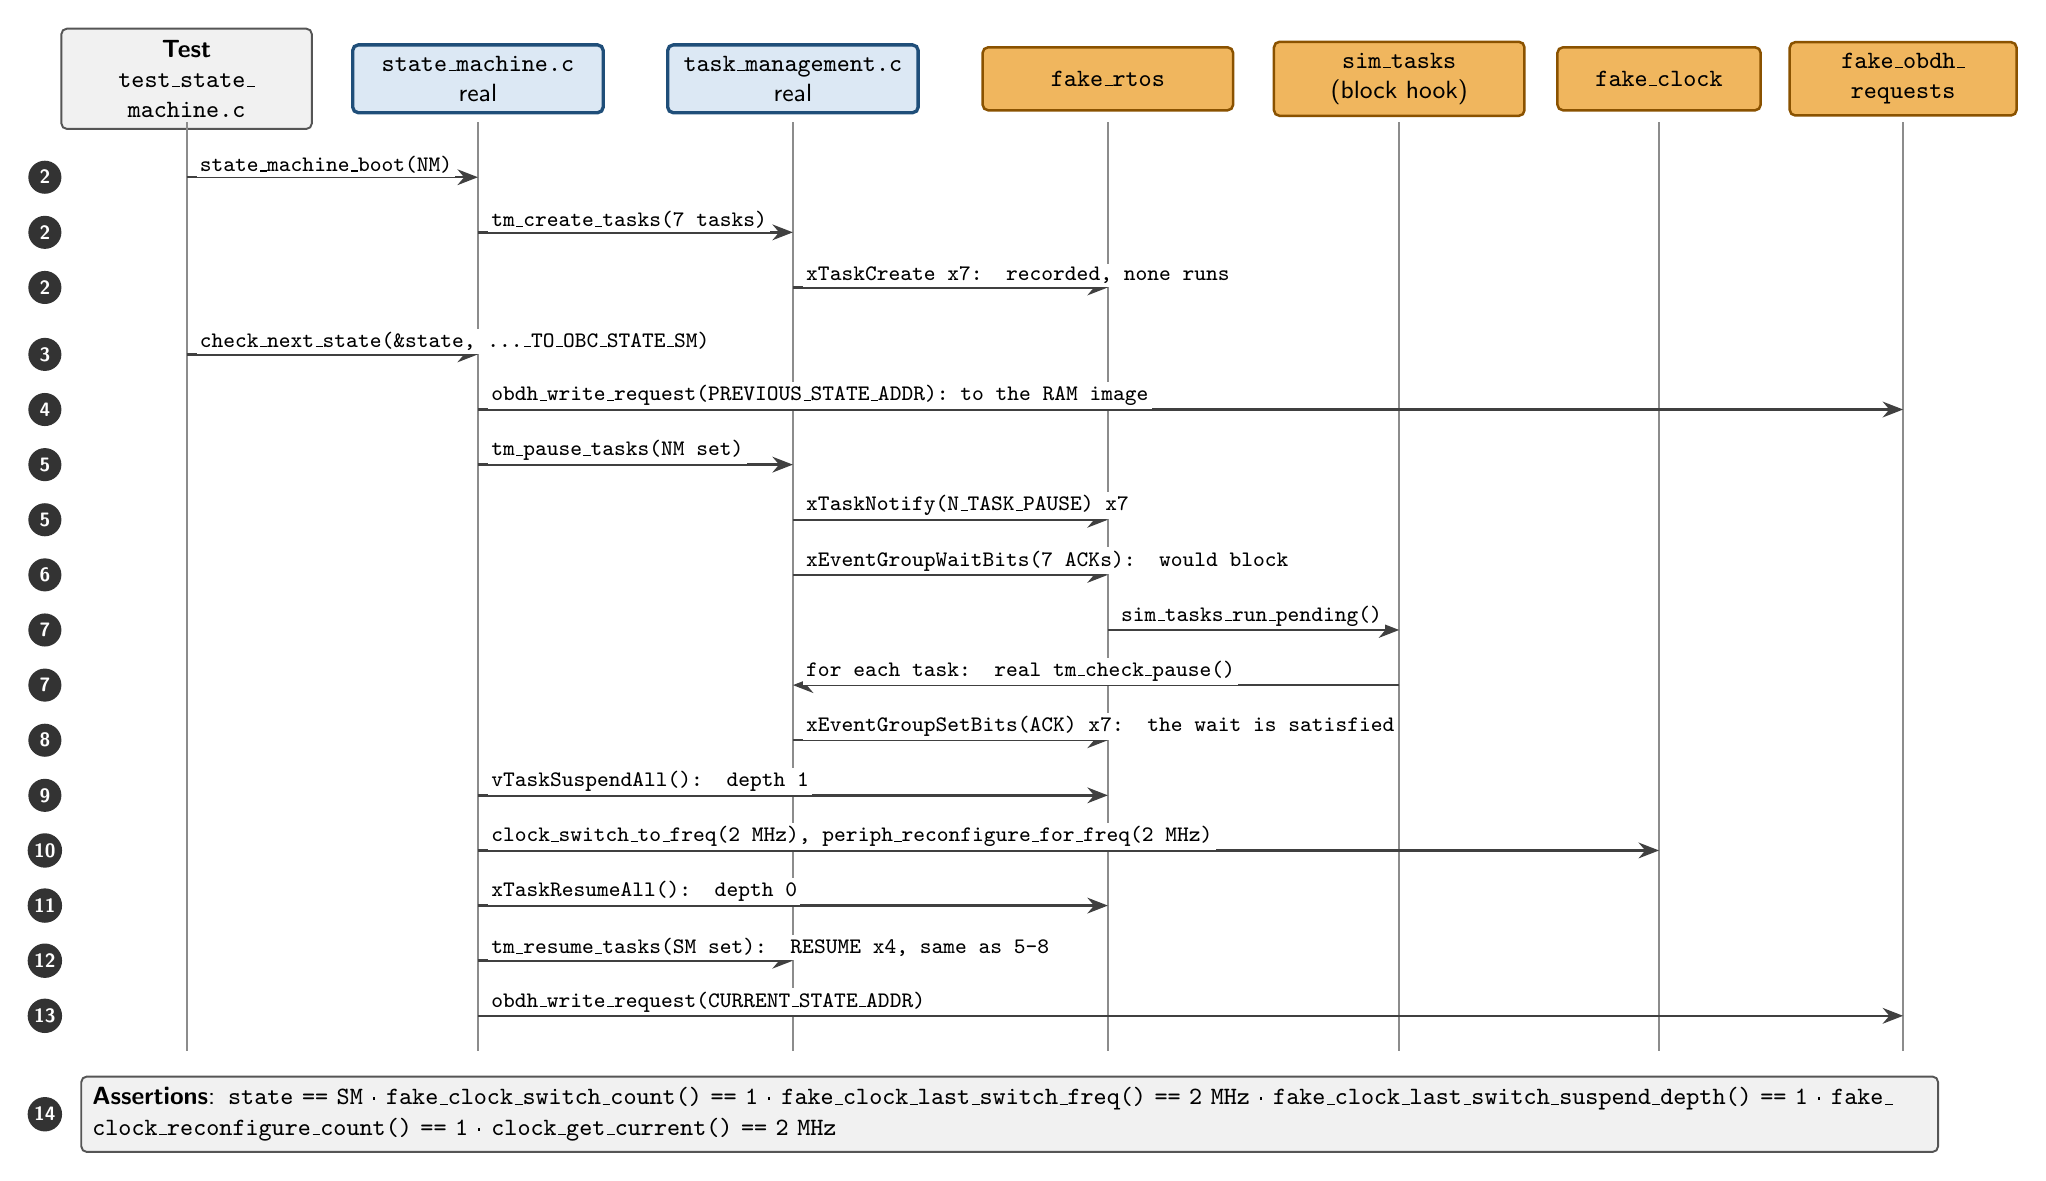
\begin{tikzpicture}[
  hd/.style={box, text width=2.9cm, minimum height=1.0cm, font=\sffamily\small},
  seql/.style={anchor=south west, fill=white, inner sep=1.2pt, font=\ttfamily\footnotesize},
  stepn/.style={circle, fill=black!80, text=white, font=\sffamily\bfseries\scriptsize, inner sep=1.2pt, minimum size=4.2mm},
  ]
\def\xT{1.9}\def\xS{5.6}\def\xM{9.6}\def\xR{13.6}\def\xI{17.3}\def\xC{20.6}\def\xO{23.7}
\node[hd, tool] at (\xT,0) {\textbf{Test}\\\cd{test\_state\_machine.c}};
\node[hd, prod] at (\xS,0) {\cd{state\_machine.c}\\real};
\node[hd, prod] at (\xM,0) {\cd{task\_management.c}\\real};
\node[hd, fake] at (\xR,0) {\cd{fake\_rtos}};
\node[hd, fake] at (\xI,0) {\cd{sim\_tasks}\\(block hook)};
\node[hd, fake, text width=2.3cm] at (\xC,0) {\cd{fake\_clock}};
\node[hd, fake, text width=2.6cm] at (\xO,0) {\cd{fake\_obdh\_}\\\cd{requests}};
\foreach \x in {\xT,\xS,\xM,\xR,\xI,\xC,\xO} \draw[black!45, line width=0.8pt] (\x,-0.55) -- (\x,-12.35);

% msg: #1 x origin, #2 x destination, #3 y, #4 number, #5 text
\newcommand{\msg}[5]{%
  \draw[arr] (#1,#3) -- (#2,#3);
  \pgfmathsetmacro{\xmin}{min(#1,#2)+0.12}
  \node[seql] at (\xmin,#3) {#5};
  \node[stepn] at (0.1,#3) {#4};}

\msg{\xT}{\xS}{-1.25}{2}{state\_machine\_boot(NM)}
\msg{\xS}{\xM}{-1.95}{2}{tm\_create\_tasks(7 tasks)}
\msg{\xM}{\xR}{-2.65}{2}{xTaskCreate x7: recorded, none runs}
\msg{\xT}{\xS}{-3.50}{3}{check\_next\_state(\&state, ...\_TO\_OBC\_STATE\_SM)}
\msg{\xS}{\xO}{-4.20}{4}{obdh\_write\_request(PREVIOUS\_STATE\_ADDR): to the RAM image}
\msg{\xS}{\xM}{-4.90}{5}{tm\_pause\_tasks(NM set)}
\msg{\xM}{\xR}{-5.60}{5}{xTaskNotify(N\_TASK\_PAUSE) x7}
\msg{\xM}{\xR}{-6.30}{6}{xEventGroupWaitBits(7 ACKs): would block}
\msg{\xR}{\xI}{-7.00}{7}{sim\_tasks\_run\_pending()}
\msg{\xI}{\xM}{-7.70}{7}{for each task: real tm\_check\_pause()}
\msg{\xM}{\xR}{-8.40}{8}{xEventGroupSetBits(ACK) x7: the wait is satisfied}
\msg{\xS}{\xR}{-9.10}{9}{vTaskSuspendAll(): depth 1}
\msg{\xS}{\xC}{-9.80}{10}{clock\_switch\_to\_freq(2 MHz), periph\_reconfigure\_for\_freq(2 MHz)}
\msg{\xS}{\xR}{-10.50}{11}{xTaskResumeAll(): depth 0}
\msg{\xS}{\xM}{-11.20}{12}{tm\_resume\_tasks(SM set): RESUME x4, same as 5-8}
\msg{\xS}{\xO}{-11.90}{13}{obdh\_write\_request(CURRENT\_STATE\_ADDR)}

\node[stepn] at (0.1,-13.15) {14};
\node[box, fill=cBg, draw=cGrey, align=left, text width=23.3cm, font=\sffamily\small, anchor=west] at (0.55,-13.15)
  {\textbf{Assertions}: \cd{state == SM} · \cd{fake\_clock\_switch\_count() == 1} · \cd{fake\_clock\_last\_switch\_freq() == 2 MHz} ·
   \cd{fake\_clock\_last\_switch\_suspend\_depth() == 1} · \cd{fake\_clock\_reconfigure\_count() == 1} · \cd{clock\_get\_current() == 2 MHz}};
\end{tikzpicture}
\caption{The calls behind \cd{test\_NM\_to\_SM\_switches\_clock\_to\_2MHz\_once}. Blue
columns: real flight code. Ochre columns: fakes. The numbers are the steps in the text. \textbf{What to
take away:} the test only makes two calls (steps 2 and 3) and then asks the fakes what happened. Everything
in between is the flight code running just as it would on the satellite; step 7 is the one that
replaces the scheduler and gives the other tasks their turn.}
\label{fig:seq}
\end{slidefig}

\subsection{A telecommand: \texorpdfstring{\cd{TC\_UPLOAD\_EPS\_TH}}{TC\_UPLOAD\_EPS\_TH}}

The tests of the telecommand catalogue all have the same shape: a frame is sent to the
real \cd{tc\_process()} and \emph{everything} it did is checked. This is the test for the
telecommand that uploads the three power thresholds:
\begin{lstlisting}[language=C]
void test_TC_UPLOAD_EPS_TH_writes_flash_and_notifies_eps(void)
{
    const uint8_t th[3] = { 10, 20, 30 };

    send_tc(TC_UPLOAD_EPS_TH, th, sizeof(th));

    TEST_ASSERT_EQUAL_INT(1, fake_obdh_call_count());
    fake_obdh_call_t c = fake_obdh_call_at(0);
    TEST_ASSERT_EQUAL_INT(FAKE_OBDH_WRITE, c.op);
    TEST_ASSERT_EQUAL_HEX32(EPS_THRESHOLDS_ADDR, c.addr);
    TEST_ASSERT_EQUAL_UINT(3, c.len);
    TEST_ASSERT_EQUAL_HEX8_ARRAY(th, fake_obdh_flash(EPS_THRESHOLDS_ADDR), 3);
    assert_only_notified(task(TM_TASK_EPS), N_EPS_NEW_THRESHOLDS);
}
\end{lstlisting}

\cd{send\_tc()} is a helper in the suite: it builds an \cd{AIR\_TC} frame with the body
\cd{[BODY\_VER, TC\_ID, params...]} and passes it to \cd{tc\_process()}, just as
\cd{comms\_task} does on the satellite. The effects end up spread over three fakes
(figure~\ref{fig:tc}), and the test reads them:
\begin{itemize}
\item \textbf{Flash}: there was exactly one call to the OBDH, a 3-byte \cd{WRITE} to
  \cd{EPS\_THRESHOLDS\_ADDR}, and the flash image contains \cd{10, 20, 30}.
\item \textbf{Notifications}: \cd{assert\_only\_notified()} checks that the EPS task received
  \cd{N\_EPS\_NEW\_THRESHOLDS} and that \emph{none of the other} 8 tasks received anything. Checking
  also what did \emph{not} happen is what makes the test useful.
\item \textbf{Transmit queue}: in other telecommands, the test pops the TM or NACK frame
  from the queue, decodes it and checks its fields.
\end{itemize}

The neighbouring test, \cd{test\_TC\_UPLOAD\_EPS\_TH\_short\_is\_rejected}, sends the same
telecommand without the three bytes. The flight code does not check the length and stores
leftover bytes as thresholds: this is KI-8, and the test is parked as a \cd{KNOWN BUG}.

\begin{figure}[H]
\centering
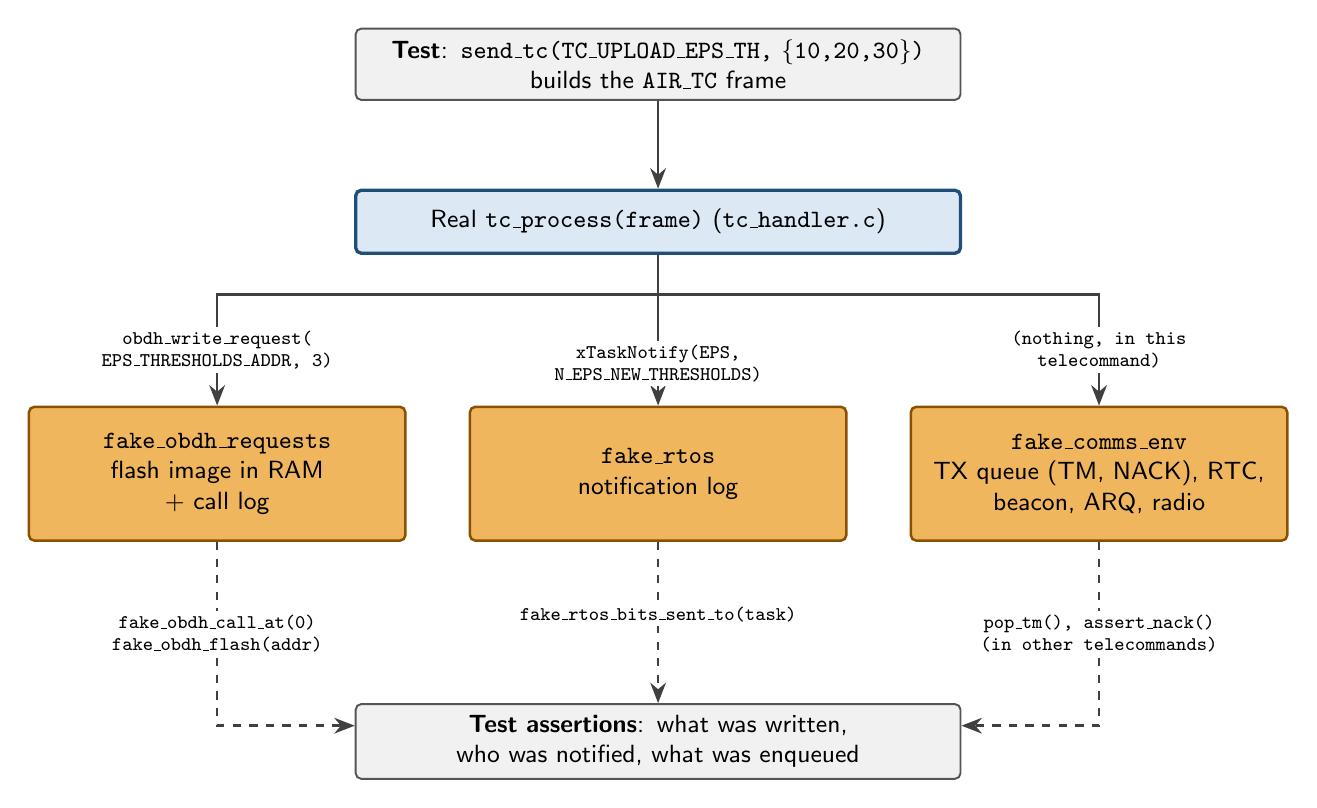
\begin{tikzpicture}[
  fk/.style={fake, text width=4.5cm, minimum height=1.7cm, font=\sffamily\small},
  rd/.style={font=\ttfamily\scriptsize, fill=white, inner sep=1.5pt, align=center},
  ]
\node[tool, text width=7.4cm, font=\sffamily\small] (t) at (0,0) {\textbf{Test}: \cd{send\_tc(TC\_UPLOAD\_EPS\_TH, \{10,20,30\})}\\builds the \cd{AIR\_TC} frame};
\node[prod, text width=7.4cm, font=\sffamily\small] (p) at (0,-2.0) {Real \textbf{\cd{tc\_process(frame)}} (\cd{tc\_handler.c})};
\node[fk] (f1) at (-5.6,-5.2) {\textbf{\cd{fake\_obdh\_requests}}\\flash image in RAM\\+ call log};
\node[fk] (f2) at (0,-5.2) {\textbf{\cd{fake\_rtos}}\\notification log};
\node[fk] (f3) at (5.6,-5.2) {\textbf{\cd{fake\_comms\_env}}\\TX queue (TM, NACK), RTC,\\beacon, ARQ, radio};
\node[tool, text width=7.4cm, font=\sffamily\small] (a) at (0,-8.6) {\textbf{Test assertions}: what was written, who was notified, what was enqueued};

\draw[arr] (t) -- (p);
\draw[arr] (p.south) -- ++(0,-0.5) -| node[rd, pos=0.75] {obdh\_write\_request(\\EPS\_THRESHOLDS\_ADDR, 3)} (f1.north);
\draw[arr] (p.south) -- node[rd, pos=0.72] {xTaskNotify(EPS,\\N\_EPS\_NEW\_THRESHOLDS)} (f2.north);
\draw[arr] (p.south) -- ++(0,-0.5) -| node[rd, pos=0.75] {(nothing, in this\\telecommand)} (f3.north);
\draw[darr] (f1.south) |- node[rd, pos=0.25] {fake\_obdh\_call\_at(0)\\fake\_obdh\_flash(addr)} ([yshift=2mm]a.west);
\draw[darr] (f2.south) -- node[rd, pos=0.45] {fake\_rtos\_bits\_sent\_to(task)} (a.north);
\draw[darr] (f3.south) |- node[rd, pos=0.25] {pop\_tm(), assert\_nack()\\(in other telecommands)} ([yshift=2mm]a.east);
\end{tikzpicture}
\caption{Where the effects of a telecommand end up and how the test reads them. Solid arrows: what
the flight code does. Dashed arrows: what the test asks. \textbf{What to take away:} the flight code
writes to flash, notifies tasks and enqueues frames exactly as on the satellite, but each of these
outputs ends up in a fake that records it. A catalogue test checks all three.}
\label{fig:tc}
\end{figure}

\subsection{A radio test in a nutshell}

The suites \cd{test\_saw} and \cd{test\_arq} test protocols that need someone on the other
side. \cd{fake\_link} acts as the radio and the ground station at once: it records every frame the
code transmits and lets you install a ``responder'', a test function that receives the
transmitted frame and decides what the ground replies (an ACK, a NACK, nothing, a corrupted frame).
For example, \cd{test\_no\_reply\_retransmits\_3\_times\_then\_times\_out} installs no
responder and checks that \cd{saw\_send()} transmits the frame, retransmits it three times and
ends up returning a timeout; time ``passes'' because the fake FreeRTOS advances the tick on every
wait, without really waiting.

\clearpage
% =====================================================================
\section{The fake FreeRTOS}\label{sec:rtos}

\cd{fake\_rtos.c} (500 lines) implements the FreeRTOS API that the firmware uses:
tasks, indexed notifications, queues, event groups, mutexes, software
timers, critical sections, \cd{vTaskSuspendAll} and the tick. It is the most important piece
of the infrastructure. It differs from the real FreeRTOS in three ways:

\begin{enumerate}
\item \textbf{Nothing runs in parallel.} \cd{xTaskCreate} records the task but
  \emph{never} runs its function. The ``running'' task is the one the test chooses with
  \cd{fake\_rtos\_set\_current\_task()}; at the start it is the test itself.
\item \textbf{Blocking is simulated} (figure~\ref{fig:rtos}). When a call would have
  to wait, the fake calls a \emph{block hook} once; if the call still cannot be
  satisfied afterwards, it advances the tick and returns a timeout, or, if the wait was \cd{portMAX\_DELAY}, it makes
  the test fail with ``deadlock'', because on the satellite that task would hang
  forever.
\item \textbf{It records everything.} Every notification, every queue item and every timer is
  logged, and the test can query them.
\end{enumerate}

\begin{table}[H]
\centering\small
\begin{tabularx}{\textwidth}{@{}>{\raggedright\arraybackslash}p{2.4cm}>{\raggedright\arraybackslash}X@{}}
\toprule
Purpose & Test functions\\
\midrule
Control & \cd{fake\_rtos\_reset()}, \cd{fake\_rtos\_set\_current\_task(t)}, \cd{fake\_rtos\_set\_block\_hook(fn)},
  \cd{fake\_rtos\_set\_tick(t)}, \cd{fake\_rtos\_advance\_ticks(dt)}, \cd{fake\_rtos\_fire\_timer(t)}\\
Inspect & \cd{fake\_rtos\_tasks\_created()}, \cd{fake\_rtos\_find\_task(name)}, \cd{fake\_rtos\_task\_alive(t)},
  \cd{fake\_rtos\_notify\_pending(t, idx)}, \cd{fake\_rtos\_notify\_value(t, idx)}, \cd{fake\_rtos\_bits\_sent\_to(t)},
  \cd{fake\_rtos\_notify\_log\_count()} / \cd{\_at(i)}, \cd{fake\_rtos\_queue\_items(q)},
  \cd{fake\_rtos\_timer\_period(t)}, \cd{fake\_rtos\_timer\_active(t)}\\
Inject failures & \cd{fake\_rtos\_fail\_task\_create\_at(n)}, \cd{fake\_rtos\_fail\_next\_queue\_create()},
  \cd{fake\_rtos\_fail\_next\_event\_group\_create()}\\
Balance & \cd{fake\_rtos\_critical\_depth()}, \cd{fake\_rtos\_suspend\_all\_depth()} (\cd{tearDown()} checks that they are 0)\\
Deadlocks & \cd{fake\_rtos\_expect\_deadlock(true)} (only records it), \cd{fake\_rtos\_deadlock\_detected()}\\
\bottomrule
\end{tabularx}
\caption{The control and inspection API of \cd{fake\_rtos} (\cd{test/mocks/fake\_rtos.h}).}
\end{table}

\textbf{Other rules.} \cd{vTaskDelay} only advances the tick; 1 tick is 1\,ms, as on the
satellite. Software timers do not fire on their own: only with
\cd{fake\_rtos\_fire\_timer()}. \cd{configASSERT} makes the test fail with file and line and,
as in the real FreeRTOS, it triggers on \cd{xQueueCreate} with length 0 or on
\cd{xEventGroupWaitBits} with no bits.

\textbf{\cd{sim\_tasks}: the most used block hook.} When the OBC pauses or resumes tasks, it sends
a notification and waits for the ACKs in an event group. Since no task runs
on its own, the ACK would never arrive. \cd{sim\_tasks\_run\_pending()} solves this (steps 7 and 8 of
section~\ref{sec:trace}). With \cd{sim\_tasks\_set\_unresponsive(mask)} you can simulate a
stuck task that does not answer, to test the ACK timeout and the restart by health monitoring.

\textbf{Where it falls short.} Since there is a single thread, the fake does not model races between tasks,
priorities, interrupts or stacks. It is also not strict enough in two known places: it accepts
timers with period 0 (the real FreeRTOS does a \cd{configASSERT}) and event group bits
reserved by the kernel. These are pending improvements (section~\ref{sec:roadmap}).

% ---------------------------------------------------------------- FIGURA: block_until
\begin{figure}[p]
\centering
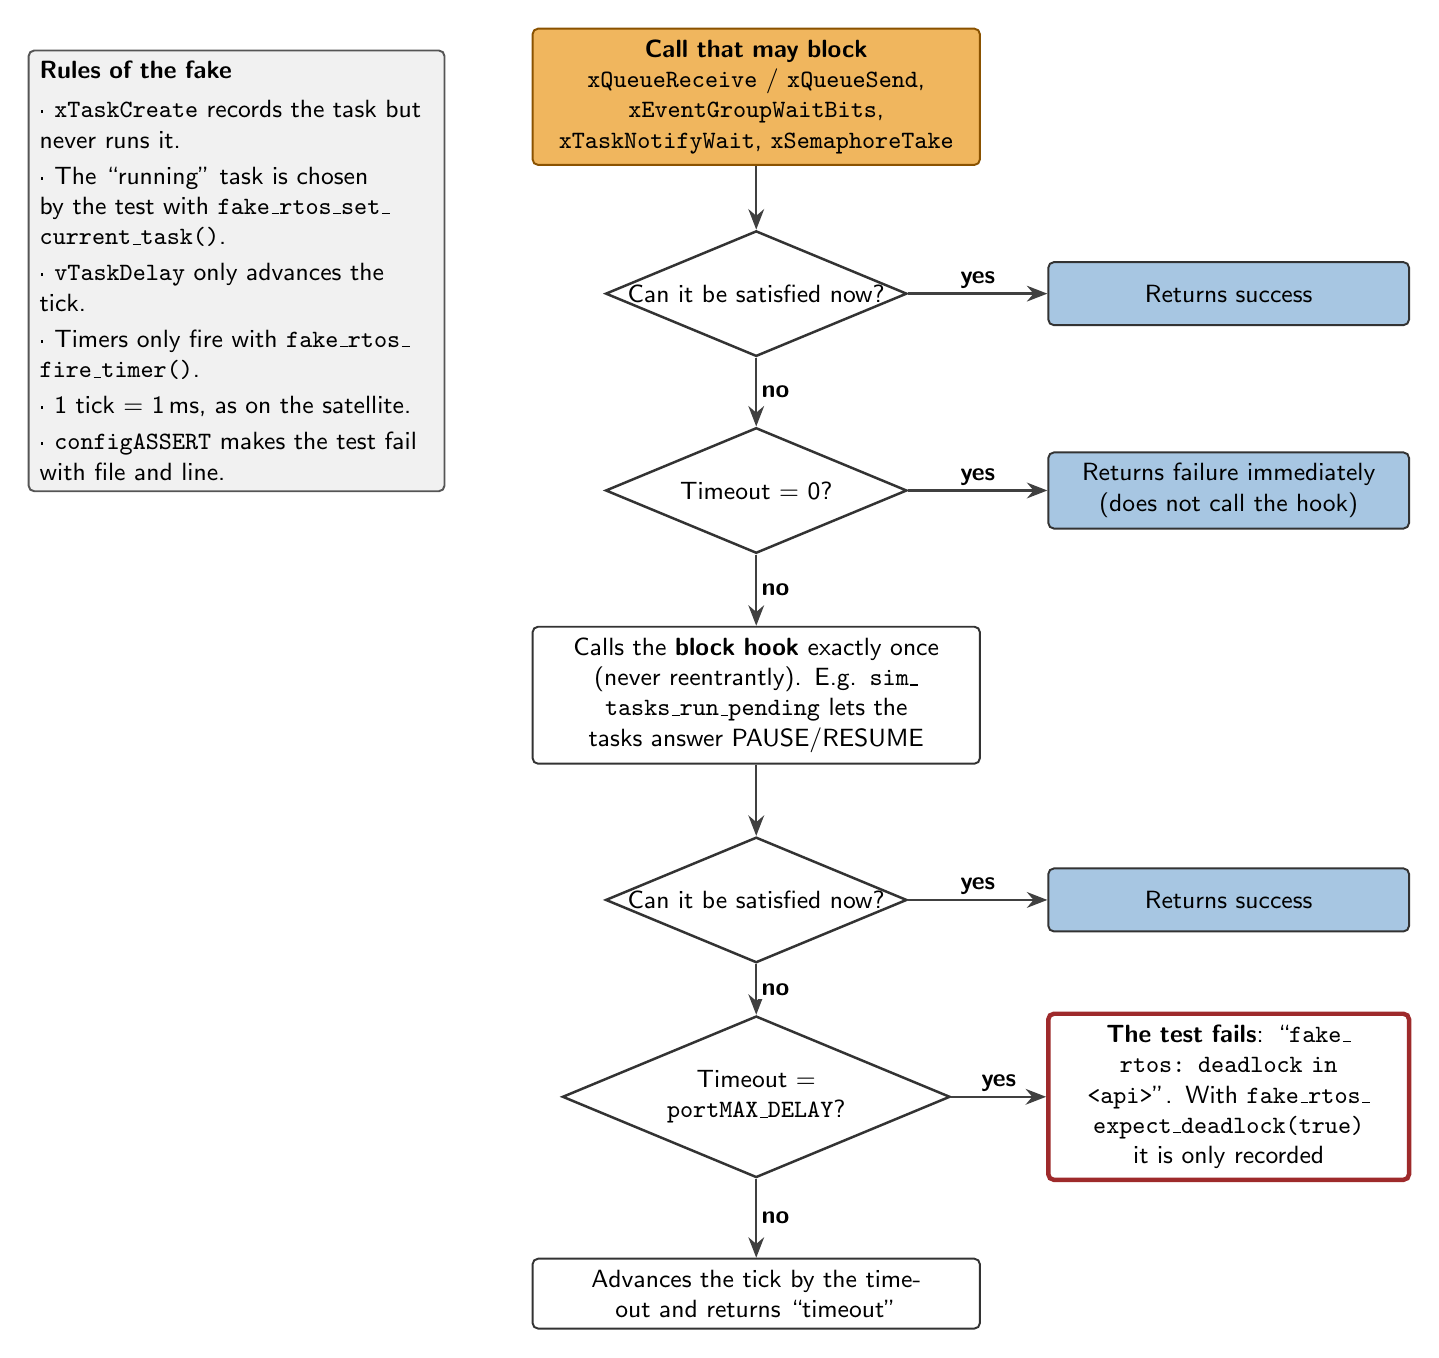
\begin{tikzpicture}[
  act/.style={box, fill=white, draw=black!80, text width=5.4cm, font=\sffamily\small},
  okn/.style={box, fill=cCovPart, draw=black!80, text width=4.3cm, font=\sffamily\small},
  bad/.style={box, fill=white, draw=cWarn, line width=1.6pt, text width=4.3cm, font=\sffamily\small},
  ]
\node[act, fill=cFakeL, draw=cFakeD] (s) at (0,0) {\textbf{Call that may block}\\
  \cd{xQueueReceive} / \cd{xQueueSend}, \cd{xEventGroupWaitBits}, \cd{xTaskNotifyWait}, \cd{xSemaphoreTake}};
\node[decision] (d1) at (0,-2.5) {Can it be satisfied now?};
\node[okn] (o1) at (6.0,-2.5) {Returns success};
\node[decision] (d2) at (0,-5.0) {Timeout = 0?};
\node[okn] (o0) at (6.0,-5.0) {Returns failure immediately (does not call the hook)};
\node[act] (h) at (0,-7.6) {Calls the \textbf{block hook} exactly once (never reentrantly).
  E.g. \cd{sim\_tasks\_run\_pending} lets the tasks answer PAUSE/RESUME};
\node[decision] (d3) at (0,-10.2) {Can it be satisfied now?};
\node[okn] (o2) at (6.0,-10.2) {Returns success};
\node[decision] (d4) at (0,-12.7) {Timeout = \cd{portMAX\_DELAY}?};
\node[bad] (dl) at (6.0,-12.7) {\textbf{The test fails}: ``\cd{fake\_rtos: deadlock in <api>}''.
  With \cd{fake\_rtos\_expect\_deadlock(true)} it is only recorded};
\node[act] (to) at (0,-15.2) {Advances the tick by the timeout and returns ``timeout''};

\draw[arr] (s) -- (d1);
\draw[arr] (d1) -- node[lbl, above] {yes} (o1);
\draw[arr] (d1) -- node[lbl, right] {no} (d2);
\draw[arr] (d2) -- node[lbl, above] {yes} (o0);
\draw[arr] (d2) -- node[lbl, right] {no} (h);
\draw[arr] (h) -- (d3);
\draw[arr] (d3) -- node[lbl, above] {yes} (o2);
\draw[arr] (d3) -- node[lbl, right] {no} (d4);
\draw[arr] (d4) -- node[lbl, above] {yes} (dl);
\draw[arr] (d4) -- node[lbl, right] {no} (to);

\node[box, fill=cBg, draw=cGrey, align=left, text width=5.0cm, font=\sffamily\small, anchor=north] (rules) at (-6.6,0.6)
  {\textbf{Rules of the fake}\\[3pt]
   · \cd{xTaskCreate} records the task but never runs it.\\[2pt]
   · The ``running'' task is chosen by the test with \cd{fake\_rtos\_set\_current\_task()}.\\[2pt]
   · \cd{vTaskDelay} only advances the tick.\\[2pt]
   · Timers only fire with \cd{fake\_rtos\_fire\_timer()}.\\[2pt]
   · 1 tick = 1\,ms, as on the satellite.\\[2pt]
   · \cd{configASSERT} makes the test fail with file and line.};
\end{tikzpicture}
\caption{How \cd{fake\_rtos} resolves a call that would block (the \cd{block\_until} function in
\cd{fake\_rtos.c}). \textbf{What to take away:} a test never hangs. Either the hook makes the other tasks
``run'' and the wait is satisfied, or time jumps to the timeout, or, if the
wait was infinite, the test fails and says where a deadlock would have happened on the satellite.}
\label{fig:rtos}
\end{figure}

\clearpage
% =====================================================================
\section{The flash and communications fakes}\label{sec:fakes}

Figure~\ref{fig:fakes} is the complete map: which fake replaces which real module and
which suites use it.

\textbf{What is always linked.} \cd{pocat\_add\_suite()} adds \cd{fake\_rtos.c} and
\cd{fake\_hal.c} to all suites (``R'' in the tables), except \cd{test\_ht\_handling}.

\textbf{\emph{Weak} symbols.} \cd{stub\_task\_entries.c} defines the 7 task entry functions
(\cd{payload\_task}... \cd{beacon\_task}) as \cd{\_\_attribute\_\_((weak))}. If a
suite includes the real task (for example \cd{obdh.c}), the real definition wins without a
duplicate symbol error. \cd{fake\_comms\_env.c} does the same with the beacon globals,
\cd{beacon\_set\_period()}, \cd{arq\_begin\_dl()} and \cd{arq\_arm\_ul()}: this is why
\cd{test\_beacon} and \cd{test\_arq} can compile the real \cd{beacon.c} or \cd{arq.c}.

% ---------------------------------------------------------------- FIGURA: mapa de fakes
\begin{slidefig}
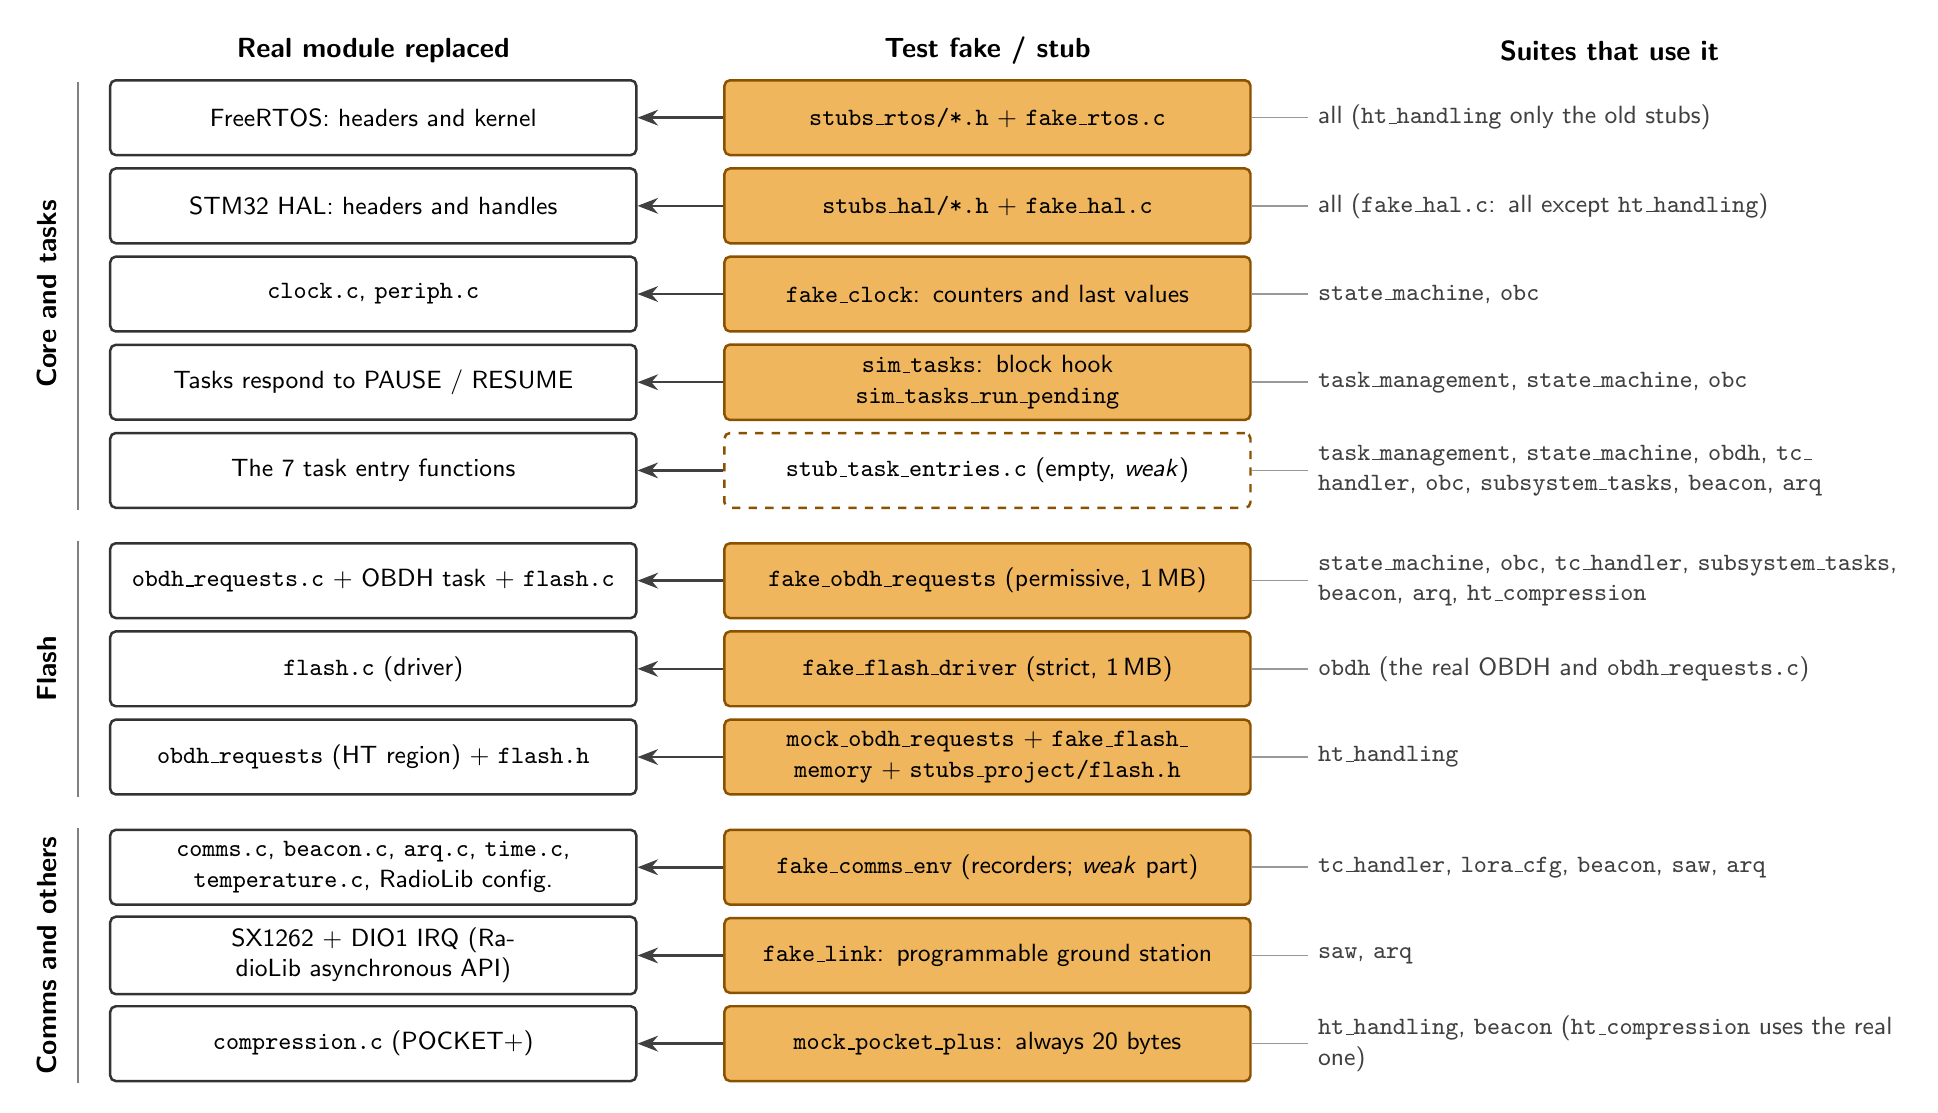
\begin{tikzpicture}[
  rm/.style={real, text width=6.4cm, minimum height=0.95cm, font=\sffamily\small},
  fk/.style={fake, text width=6.4cm, minimum height=0.95cm, font=\sffamily\small},
  sk/.style={stub, text width=6.4cm, minimum height=0.95cm, font=\sffamily\small},
  su/.style={note, text width=7.4cm, font=\sffamily\small},
  grp/.style={font=\sffamily\bfseries, rotate=90, anchor=center},
  ]
\def\xa{4.5}\def\xb{12.3}\def\xc{20.2}\def\dy{1.12}
\node[head, font=\sffamily\bfseries] at (\xa,0.85) {Real module replaced};
\node[head, font=\sffamily\bfseries] at (\xb,0.85) {Test fake / stub};
\node[head, font=\sffamily\bfseries] at (\xc,0.85) {Suites that use it};

% group A
\node[rm] (a1) at (\xa,0)        {FreeRTOS: headers and kernel};
\node[fk] (b1) at (\xb,0)        {\cd{stubs\_rtos/*.h} + \cd{fake\_rtos.c}};
\node[su] (c1) at (\xc,0)        {all (\cd{ht\_handling} only the old stubs)};
\node[rm] (a2) at (\xa,-\dy)     {STM32 HAL: headers and handles};
\node[fk] (b2) at (\xb,-\dy)     {\cd{stubs\_hal/*.h} + \cd{fake\_hal.c}};
\node[su] (c2) at (\xc,-\dy)     {all (\cd{fake\_hal.c}: all except \cd{ht\_handling})};
\node[rm] (a3) at (\xa,-2*\dy)   {\cd{clock.c}, \cd{periph.c}};
\node[fk] (b3) at (\xb,-2*\dy)   {\cd{fake\_clock}: counters and last values};
\node[su] (c3) at (\xc,-2*\dy)   {\cd{state\_machine}, \cd{obc}};
\node[rm] (a4) at (\xa,-3*\dy)   {Tasks respond to PAUSE / RESUME};
\node[fk] (b4) at (\xb,-3*\dy)   {\cd{sim\_tasks}: block hook \cd{sim\_tasks\_run\_pending}};
\node[su] (c4) at (\xc,-3*\dy)   {\cd{task\_management}, \cd{state\_machine}, \cd{obc}};
\node[rm] (a5) at (\xa,-4*\dy)   {The 7 task entry functions};
\node[sk] (b5) at (\xb,-4*\dy)   {\cd{stub\_task\_entries.c} (empty, \emph{weak})};
\node[su] (c5) at (\xc,-4*\dy)   {\cd{task\_management}, \cd{state\_machine}, \cd{obdh}, \cd{tc\_handler}, \cd{obc}, \cd{subsystem\_tasks}, \cd{beacon}, \cd{arq}};
% group B
\node[rm] (a6) at (\xa,-5.25*\dy){\cd{obdh\_requests.c} + OBDH task + \cd{flash.c}};
\node[fk] (b6) at (\xb,-5.25*\dy){\cd{fake\_obdh\_requests} (permissive, 1\,MB)};
\node[su] (c6) at (\xc,-5.25*\dy){\cd{state\_machine}, \cd{obc}, \cd{tc\_handler}, \cd{subsystem\_tasks}, \cd{beacon}, \cd{arq}, \cd{ht\_compression}};
\node[rm] (a7) at (\xa,-6.25*\dy){\cd{flash.c} (driver)};
\node[fk] (b7) at (\xb,-6.25*\dy){\cd{fake\_flash\_driver} (strict, 1\,MB)};
\node[su] (c7) at (\xc,-6.25*\dy){\cd{obdh} (the real OBDH and \cd{obdh\_requests.c})};
\node[rm] (a8) at (\xa,-7.25*\dy){\cd{obdh\_requests} (HT region) + \cd{flash.h}};
\node[fk] (b8) at (\xb,-7.25*\dy){\cd{mock\_obdh\_requests} + \cd{fake\_flash\_memory} + \cd{stubs\_project/flash.h}};
\node[su] (c8) at (\xc,-7.25*\dy){\cd{ht\_handling}};
% group C
\node[rm] (a9) at (\xa,-8.5*\dy) {\cd{comms.c}, \cd{beacon.c}, \cd{arq.c}, \cd{time.c}, \cd{temperature.c}, RadioLib config.};
\node[fk] (b9) at (\xb,-8.5*\dy) {\cd{fake\_comms\_env} (recorders; \emph{weak} part)};
\node[su] (c9) at (\xc,-8.5*\dy) {\cd{tc\_handler}, \cd{lora\_cfg}, \cd{beacon}, \cd{saw}, \cd{arq}};
\node[rm] (a10) at (\xa,-9.5*\dy){SX1262 + DIO1 IRQ (RadioLib asynchronous API)};
\node[fk] (b10) at (\xb,-9.5*\dy){\cd{fake\_link}: programmable ground station};
\node[su] (c10) at (\xc,-9.5*\dy){\cd{saw}, \cd{arq}};
\node[rm] (a11) at (\xa,-10.5*\dy){\cd{compression.c} (POCKET+)};
\node[fk] (b11) at (\xb,-10.5*\dy){\cd{mock\_pocket\_plus}: always 20 bytes};
\node[su] (c11) at (\xc,-10.5*\dy){\cd{ht\_handling}, \cd{beacon} (\cd{ht\_compression} uses the real one)};

\foreach \i in {1,...,11}{ \draw[arr] (b\i.west) -- (a\i.east); \draw[black!40, line width=0.6pt] (b\i.east) -- (c\i.west); }

\node[grp] at (0.35,-2*\dy)    {Core and tasks};
\node[grp] at (0.35,-6.25*\dy) {Flash};
\node[grp] at (0.35,-9.5*\dy)  {Comms and others};
\draw[black!50, line width=1pt] (0.75,0.45) -- (0.75,-4.45*\dy);
\draw[black!50, line width=1pt] (0.75,-4.8*\dy) -- (0.75,-7.7*\dy);
\draw[black!50, line width=1pt] (0.75,-8.05*\dy) -- (0.75,-10.95*\dy);
\end{tikzpicture}
\caption{Map of fakes. Each arrow goes from the fake to the real module it replaces; on the right, the suites
that link it (without the \cd{test\_} prefix). Solid border: fake with behaviour; dashed border:
empty stub. \textbf{What to take away:} \cd{fake\_rtos} and \cd{fake\_hal} are the base of almost everything; flash
has three different models depending on the suite (figure~\ref{fig:flashmodels}); and comms are tested with a
fake environment and a fake radio link that act as the satellite and the ground station.}
\label{fig:fakes}
\end{slidefig}

\subsection{The three flash models}

In the firmware, no task touches \cd{flash.c} directly: they all call
\cd{obdh\_read/write/program/erase\_program\_request}, which put the request in the queue of the
OBDH task and wait for the reply on notification index 1. In the tests, this path is
cut at three different heights, with different rules (figure~\ref{fig:flashmodels}). It is
important to know this: the same code can pass with one fake and fail with another.

\begin{table}[H]
\centering\small
\begin{tabularx}{\textwidth}{@{}>{\raggedright\arraybackslash}p{2.6cm}>{\raggedright\arraybackslash}X>{\raggedright\arraybackslash}X>{\raggedright\arraybackslash}X@{}}
\toprule
 & \cd{fake\_flash\_driver} & \cd{fake\_obdh\_requests} & \cd{mock\_obdh\_requests} + \cd{fake\_flash\_memory}\\
\midrule
Replaces & \cd{flash.c} & \cd{obdh\_requests.c} (and therefore the OBDH and \cd{flash.c}) & \cd{obdh\_requests.c}, HT region only\\
Memory & 1\,MB from \cd{0x08000000}, initially \cd{0xFF} & 1\,MB from \cd{0x08000000}, initially \cd{0xFF} & 8\,KB from \cd{HT\_BASE\_ADDR} (\cd{0x080FE000})\\
\cd{program} & alignment and length multiples of 8; destination erased; otherwise \cd{HAL\_ERROR} & bitwise AND, with no checks & strict mode: \cd{TEST\_ASSERT} on alignment 8 and on 1\fl{}0 transitions\\
\cd{write} & \cd{memcpy} (the real driver erases and rewrites the page) & \cd{memcpy} & same as \cd{erase\_program}\\
Erase & 2\,KB page & \cd{erase\_program}: page to \cd{0xFF} and then AND & 2\,KB page\\
Extras & error injection, counters, last address & log of 256 calls, error injection & power cut after N operations, error injection\\
Suites & \cd{test\_obdh} & 7 suites (fig.~\ref{fig:fakes}) & \cd{test\_ht\_handling}\\
\bottomrule
\end{tabularx}
\caption{Comparison of the three flash models.}
\label{tab:flash}
\end{table}

% ---------------------------------------------------------------- FIGURA: models de flash
\begin{slidefig}
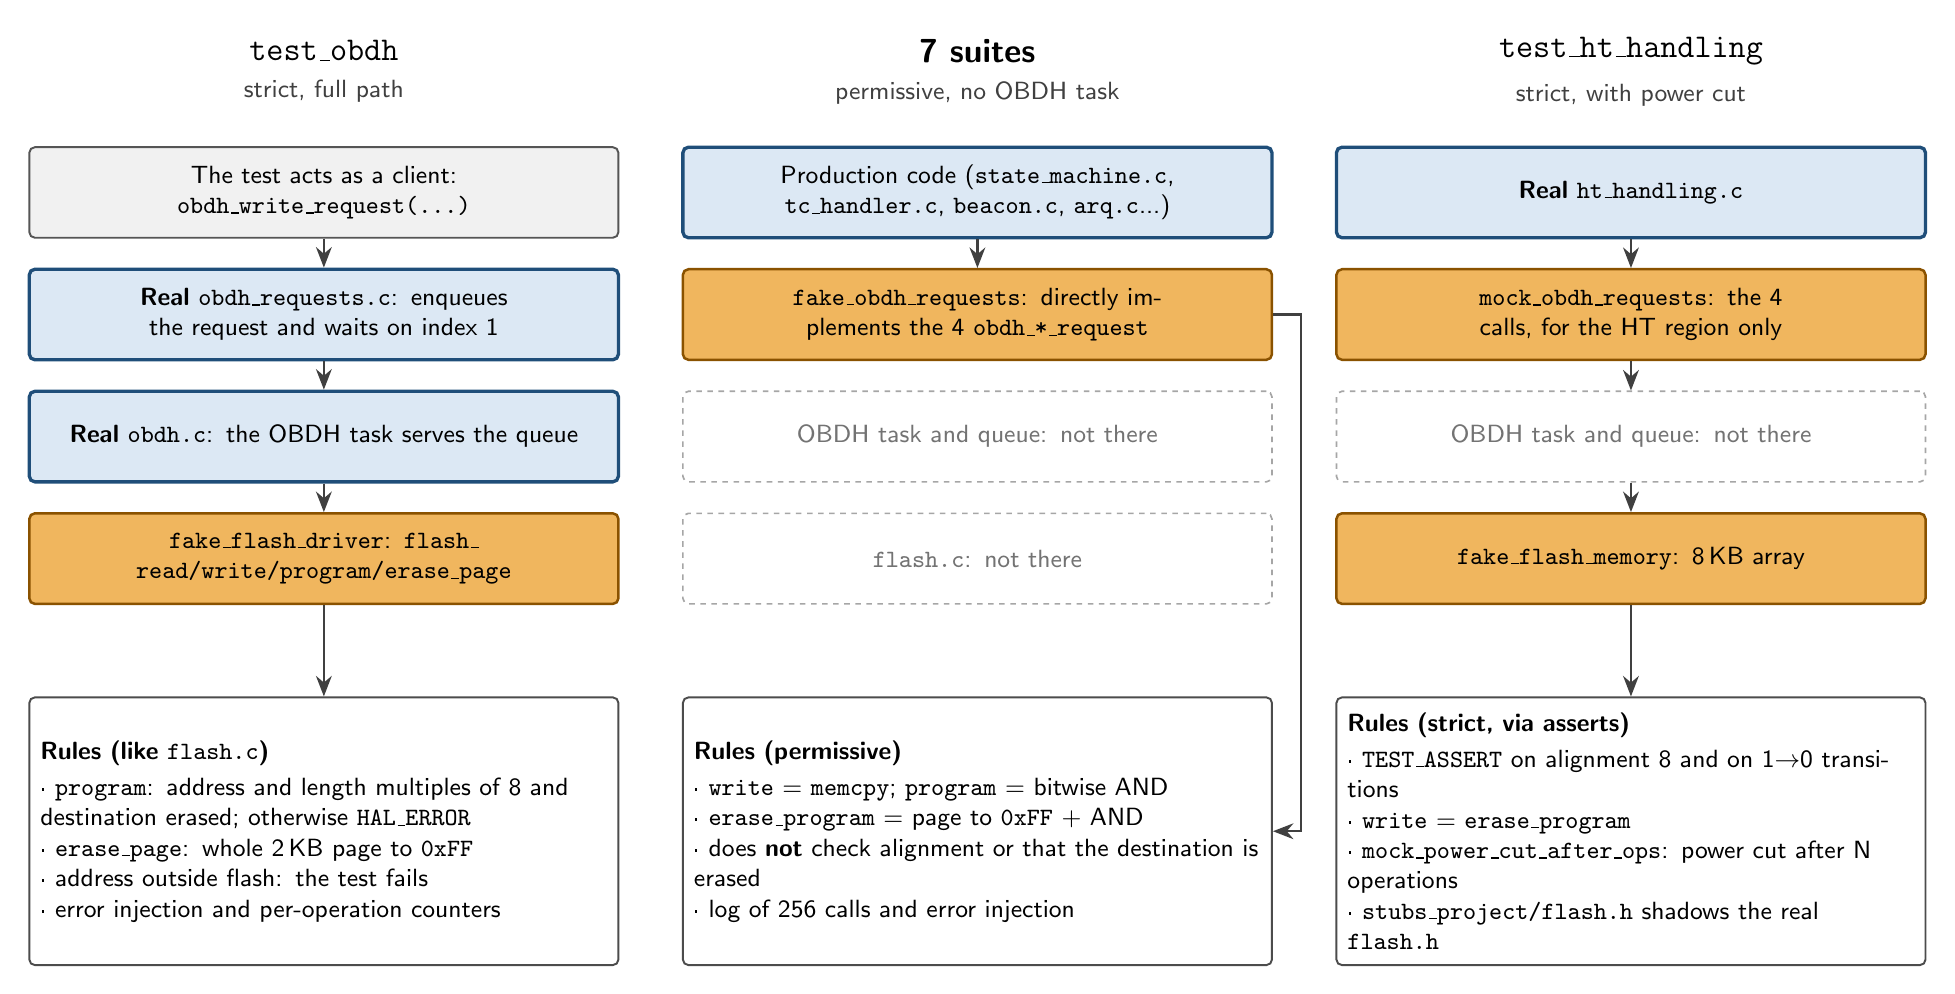
\begin{tikzpicture}[
  cc/.style={text width=7.2cm, minimum height=1.15cm, font=\sffamily\small},
  rules/.style={box, fill=white, draw=black!70, align=left, text width=7.2cm, minimum height=3.4cm, font=\sffamily\small, anchor=north},
  ]
\def\xa{4.0}\def\xb{12.3}\def\xc{20.6}\def\dy{1.55}
\node[head] (ha) at (\xa,0.2) {\cd{test\_obdh}};
\node[note, below=0mm of ha, align=center] {strict, full path};
\node[head] (hb) at (\xb,0.2) {7 suites};
\node[note, below=0mm of hb, align=center] {permissive, no OBDH task};
\node[head] (hc) at (\xc,0.2) {\cd{test\_ht\_handling}};
\node[note, below=0mm of hc, align=center] {strict, with power cut};

\node[tool, cc] (a1) at (\xa,-1.6) {The test acts as a client: \cd{obdh\_write\_request(...)}};
\node[prod, cc] (a2) at (\xa,-1.6-\dy) {\textbf{Real} \cd{obdh\_requests.c}: enqueues the request and waits on index 1};
\node[prod, cc] (a3) at (\xa,-1.6-2*\dy) {\textbf{Real} \cd{obdh.c}: the OBDH task serves the queue};
\node[fake, cc] (a4) at (\xa,-1.6-3*\dy) {\cd{fake\_flash\_driver}: \cd{flash\_read/write/program/erase\_page}};

\node[prod, cc] (b1) at (\xb,-1.6) {Production code (\cd{state\_machine.c}, \cd{tc\_handler.c}, \cd{beacon.c}, \cd{arq.c}...)};
\node[fake, cc] (b2) at (\xb,-1.6-\dy) {\cd{fake\_obdh\_requests}: directly implements the 4 \cd{obdh\_*\_request}};
\node[ghost, cc] (b3) at (\xb,-1.6-2*\dy) {OBDH task and queue: not there};
\node[ghost, cc] (b4) at (\xb,-1.6-3*\dy) {\cd{flash.c}: not there};

\node[prod, cc] (c1) at (\xc,-1.6) {\textbf{Real} \cd{ht\_handling.c}};
\node[fake, cc] (c2) at (\xc,-1.6-\dy) {\cd{mock\_obdh\_requests}: the 4 calls, for the HT region only};
\node[ghost, cc] (c3) at (\xc,-1.6-2*\dy) {OBDH task and queue: not there};
\node[fake, cc] (c4) at (\xc,-1.6-3*\dy) {\cd{fake\_flash\_memory}: 8\,KB array};

\node[rules] (a5) at (\xa,-8.0) {\textbf{Rules (like \cd{flash.c})}\\[2pt]
  · \cd{program}: address and length multiples of 8 and destination erased; otherwise \cd{HAL\_ERROR}\\
  · \cd{erase\_page}: whole 2\,KB page to \cd{0xFF}\\
  · address outside flash: the test fails\\
  · error injection and per-operation counters};
\node[rules] (b5) at (\xb,-8.0) {\textbf{Rules (permissive)}\\[2pt]
  · \cd{write} = \cd{memcpy}; \cd{program} = bitwise AND\\
  · \cd{erase\_program} = page to \cd{0xFF} + AND\\
  · does \textbf{not} check alignment or that the destination is erased\\
  · log of 256 calls and error injection};
\node[rules] (c5) at (\xc,-8.0) {\textbf{Rules (strict, via asserts)}\\[2pt]
  · \cd{TEST\_ASSERT} on alignment 8 and on 1\fl{}0 transitions\\
  · \cd{write} = \cd{erase\_program}\\
  · \cd{mock\_power\_cut\_after\_ops}: power cut after N operations\\
  · \cd{stubs\_project/flash.h} shadows the real \cd{flash.h}};

\foreach \c in {a,b,c}{\draw[arr] (\c1) -- (\c2);}
\draw[arr] (a2) -- (a3); \draw[arr] (a3) -- (a4); \draw[arr] (a4) -- (a5);
\draw[arr] (b2.east) -- ++(0.35,0) |- (b5.east);
\draw[arr] (c2) -- (c3); \draw[arr] (c3) -- (c4); \draw[arr] (c4) -- (c5);
\end{tikzpicture}
\caption{The three flash models, aligned by layer; the dashed grey boxes are layers that
are missing. \textbf{What to take away:} only \cd{test\_obdh} tests the real path client \fl{} queue \fl{} OBDH task \fl{}
driver. The other 7 suites that write to flash jump straight to a permissive memory that
accepts writes the hardware would reject. Making it strict is a pending decision
(section~\ref{sec:roadmap}).}
\label{fig:flashmodels}
\end{slidefig}

\subsection{The other fakes}
\begin{itemize}
\item \cd{fake\_hal}: defines the global handles (\cd{hiwdg}, \cd{huart4}, \cd{htim2}, \cd{htim5},
  \cd{hspi2}, \cd{hrtc}, \cd{hadc1}) and counts the calls to \cd{HAL\_IWDG\_Refresh}.
\item \cd{fake\_clock}: replaces \cd{clock\_get\_current}, \cd{clock\_switch\_to\_freq},
  \cd{systemclock\_init\_for\_freq} and \cd{periph\_*\_for\_freq}; it records counters, the last
  frequency and the \cd{vTaskSuspendAll} depth at the moment of the switch.
\item \cd{fake\_comms\_env}: everything \cd{tc\_handler.c} calls outside itself: comms TX/RX
  queues, RTC time, beacon period, ARQ, MCU sensors and radio configuration
  (queryable with \cd{fake\_radio\_last\_config()}).
\item \cd{fake\_link}: replaces the SX1262 and the DIO1 line. It records up to 64 TX frames, accepts up
  to 4 injected RX frames, has a ``responder'' that acts as the ground station (it replies to each TX at
  most once), a configurable CAD result, and lets you disable TX\_DONE.
\item \cd{mock\_pocket\_plus}: \cd{compressPacket()} copies 20 bytes and returns 20, always. It is
  deterministic (5 beacons per block), but it does not test the real format; this is why
  \cd{test\_ht\_compression} exists, which links the real \cd{compression.c}.
\item \cd{pocat\_test\_main.h}: the common \cd{main()}; it adds \cd{-l} (list) to Unity's
  \cd{-f}, \cd{-n} and \cd{-x} options.
\end{itemize}
% =====================================================================
\part{Catalog and status}

\section{The 15 suites and coverage}\label{sec:suites}

\subsection{The design layers}

The design (\cd{docs/testing/test-design.md}) proposes four layers. The first two
exist.

\begin{table}[H]
\centering\small
\begin{tabularx}{\textwidth}{@{}l>{\raggedright\arraybackslash}X>{\raggedright\arraybackslash}p{4.2cm}@{}}
\toprule
Layer & What it is & Status\\
\midrule
1 & Unit tests per module, with shared fakes. One suite per module and one CMake line per suite. & Done (15 suites)\\
2 & Telecommand catalog: \cd{test\_tc\_handler}, one \cd{test\_TC\_<NAME>\_...} test for each TC\_ID. & Done (55 tests)\\
3 & Interactive simulator on the PC (\cd{test/sim/pocat\_sim.c}) that reads commands from \cd{stdin} on top of the layer 2 fakes. & Not started (optional)\\
4 & Debug console on the board (\cd{POCAT\_DEBUG\_CONSOLE}), compiled out of the flight builds. & Not started; needs KI-7 fixed or the real radio\\
\bottomrule
\end{tabularx}
\caption{Layers of the test design.}
\end{table}

\subsection{Suite-by-suite table}

Table~\ref{tab:suites} summarizes the 15 suites registered in \cd{test/CMakeLists.txt}.
The test counts come from the \cd{POCAT\_RUN\_TEST(...)} calls in each file, and the
\cd{KNOWN BUG} counts come from the \cd{TEST\_IGNORE\_MESSAGE("KNOWN BUG ...")} lines; they match
the full run of 13/11/2026.

\begin{landscape}
\small
\setlength{\tabcolsep}{4pt}
\renewcommand{\arraystretch}{1.18}
\begin{longtable}{@{}>{\raggedright\arraybackslash}p{3.4cm} l >{\raggedright\arraybackslash}p{4.9cm} >{\raggedright\arraybackslash}p{3.3cm} >{\raggedright\arraybackslash}p{5.6cm} r >{\raggedright\arraybackslash}p{2.6cm} l@{}}
\caption{The 15 suites. ``R'' = \cd{fake\_rtos} + \cd{fake\_hal} (automatic). ``Git'': ``yes'' means the suite file is committed.}\label{tab:suites}\\
\toprule
Suite & Label & Production included (\cd{\#include}) & Production linked (\cd{SOURCES}) & Fakes & Tests & KNOWN BUG & Git\\
\midrule
\endfirsthead
\toprule
Suite & Label & Production included (\cd{\#include}) & Production linked (\cd{SOURCES}) & Fakes & Tests & KNOWN BUG & Git\\
\midrule
\endhead
\bottomrule
\endfoot
\cd{test\_ht\_handling} & comms & \cd{ht\_handling.c} & -- & \cd{stubs\_project/flash.h}, \cd{fake\_flash\_memory}, \cd{mock\_obdh\_requests}, \cd{mock\_pocket\_plus} (no R) & 14 & 0; 2 failing on purpose (KI-10, KI-11) & yes\\
\cd{test\_notifications} & infra & -- & \cd{notifications.c} & R & 10 & 0 & yes\\
\cd{test\_task\_management} & obc & \cd{task\_management.c}, \cd{health.c} & \cd{notifications.c} & R, \cd{stub\_task\_entries}, \cd{sim\_tasks} & 14 & 1 (KI-4) & yes\\
\cd{test\_state\_machine} & obc & \cd{state\_machine.c}, \cd{task\_management.c}, \cd{health.c} & \cd{notifications.c} & R, \cd{stub\_task\_entries}, \cd{sim\_tasks}, \cd{fake\_clock}, \cd{fake\_obdh\_requests} & 12 & 2 (KB-3 ×2) & yes\\
\cd{test\_comms\_frame} & comms & \cd{auth.c} & \cd{frame.c}, \cd{dedup.c} & R & 19 & 1 (KB-1) & yes\\
\cd{test\_health} & obc & \cd{health.c} & -- & R & 17 & 0 & no\\
\cd{test\_obdh} & obdh & \cd{obdh.c}, \cd{obdh\_requests.c}, \cd{task\_management.c}, \cd{health.c} & \cd{notifications.c} & R, \cd{stub\_task\_entries}, \cd{fake\_flash\_driver} & 19 & 1 (KI-5) & no\\
\cd{test\_tc\_handler} & comms & \cd{tc\_handler.c}, \cd{lora\_cfg.c}, \cd{tm\_builder.c}, \cd{task\_management.c}, \cd{health.c} & \cd{notifications.c}, \cd{frame.c}, \cd{auth.c} & R, \cd{stub\_task\_entries}, \cd{fake\_obdh\_requests}, \cd{fake\_comms\_env} & 55 & 4 (KI-8 ×2, KI-15, KI-16) & no\\
\cd{test\_lora\_cfg} & comms & \cd{lora\_cfg.c} & \cd{timing.c} & R, \cd{fake\_comms\_env} & 18 & 2 (KI-18, KI-19) & no\\
\cd{test\_obc} & obc & \cd{obc.c}, \cd{state\_machine.c}, \cd{task\_management.c}, \cd{health.c} & \cd{notifications.c} & R, \cd{stub\_task\_entries}, \cd{sim\_tasks}, \cd{fake\_clock}, \cd{fake\_obdh\_requests} & 11 & 1 (KI-26) & no\\
\cd{test\_subsystem\_tasks} & subsys & \cd{eps.c}, \cd{adcs.c}, \cd{payload.c}, \cd{task\_management.c}, \cd{health.c} & \cd{notifications.c} & R, \cd{stub\_task\_entries}, \cd{fake\_obdh\_requests} & 10 & 1 (KI-6) & no\\
\cd{test\_beacon} & comms & \cd{beacon.c}, \cd{ht\_handling.c}, \cd{lora\_cfg.c}, \cd{task\_management.c}, \cd{health.c} & \cd{notifications.c}, \cd{frame.c}, \cd{auth.c} & R, \cd{stub\_task\_entries}, \cd{fake\_obdh\_requests}, \cd{fake\_comms\_env}, \cd{mock\_pocket\_plus} & 15 & 2 (KI-15, KI-17) & no\\
\cd{test\_saw} & comms & \cd{saw.c}, \cd{lora\_cfg.c} & \cd{timing.c}, \cd{cad.c}, \cd{frame.c}, \cd{auth.c} & R, \cd{fake\_comms\_env}, \cd{fake\_link} & 11 & 1 (KI-24) & no\\
\cd{test\_arq} & comms & \cd{arq.c}, \cd{lora\_cfg.c}, \cd{task\_management.c}, \cd{health.c} & \cd{notifications.c}, \cd{timing.c}, \cd{cad.c}, \cd{frame.c}, \cd{auth.c} & R, \cd{stub\_task\_entries}, \cd{fake\_obdh\_requests}, \cd{fake\_comms\_env}, \cd{fake\_link} & 19 & 3 (KI-20, KI-21, KI-22) & no\\
\cd{test\_ht\_compression} & comms & \cd{ht\_handling.c} & \cd{compression.c} (real) & R, \cd{fake\_obdh\_requests} (with the real \cd{flash.h}) & 9 & 0 & no\\
\midrule
\textbf{Total} & & & & & \textbf{253} & \textbf{19} & 5 of 15\\
\end{longtable}
\end{landscape}

\textbf{What each suite tests, in one sentence.}
\begin{description}[style=nextline,leftmargin=0.6cm,font=\normalfont\ttfamily]
\item[test\_ht\_handling] The circular queue of historic telemetry: slots, eviction, erasing one page per lap, rebuilding in \cd{ht\_init()}, power cut and bad sector.
\item[test\_notifications] \cd{wait\_for\_notification()}, bitmap consistency and self-tests of the fake FreeRTOS (FIFO, event waiting, deadlock detection).
\item[test\_task\_management] Task table, creation sets, pause and resume protocol, deferral, ACK timeout, restart on health failure and creation failure.
\item[test\_state\_machine] Frequency per state, tasks at boot, NM\fl{}SM clock change, state persistence, and pausing the old tasks / resuming the new ones.
\item[test\_comms\_frame] Known SHA-256 and HMAC vectors, encoding and decoding of air frames, the 242/243 limit, the 16-byte ACK and the deduplication ring.
\item[test\_health] The software watchdog: period times (with tick overflow), missing heartbeats, grace period and IWDG refresh rules.
\item[test\_obdh] Client \fl{} queue \fl{} OBDH task \fl{} driver \fl{} reply on index 1; alignment, errors, full queue, ordering, pause and resume.
\item[test\_tc\_handler] The telecommand catalog (layer 2): one test per TC\_ID, unknown TC \fl{} NACK, all 256 identifiers either handled or rejected.
\item[test\_lora\_cfg] LoRa configuration: boot values, parse, scheduled commit, automatic rollback, BUSY windows, bandwidth map and reference time on air.
\item[test\_obc] \cd{setup\_obc()} (OBDH queue, IWDG and health period, tasks according to the state, saved boot time) and \cd{process\_obc()}.
\item[test\_subsystem\_tasks] The common task contract on the real \cd{process\_eps/adcs/payload()} and the reading of EPS thresholds.
\item[test\_beacon] The 19-byte beacon body, uptime, callback and timer period, TX frame on the queue and feeding of historic telemetry.
\item[test\_saw] Stop-and-wait sender: ACK, NACK, 3 retransmissions and timeout, authenticated RETX frames, foreign frames forwarded, busy CAD, TX\_DONE that never arrives.
\item[test\_arq] ARQ uplink: arming, \cd{DATA\_BEGIN}, out-of-order and duplicate blocks, ACK per window, final CRC-32, TLE write, calibration and flight parameters in flash. The downlink is not covered.
\item[test\_ht\_compression] Historic telemetry with the real POCKET+: blocks fit in the 128-byte slot, identical and random beacons, \cd{ht\_init()} after real blocks, queue wrap-around.
\end{description}

One figure from \cd{test\_ht\_compression}: with the real compressor, a 128-byte slot holds
between 20 and 25 realistic beacons, 97 if they are identical and only 2 or 3 if they are
random.

\subsection{Coverage map}

Figure~\ref{fig:arch} shows the flight software architecture colored by whether each
file has tests. The criteria are:
\begin{itemize}
\item \textbf{Has a suite}: the file is included in at least one suite that tests its logic.
\item \textbf{Partial}: only part of it is tested, or it is only exercised indirectly.
  \cd{arq.c} (only the uplink), \cd{compression.c} (no round-trip test with the ground
  decompressor, which is not in the repo), \cd{timing.c} (only through \cd{lora\_toa\_ms} and
  \cd{ack\_timeout\_ms}), \cd{cad.c} (linked into \cd{test\_saw} and \cd{test\_arq}) and
  \cd{eps.c}/\cd{adcs.c}/\cd{payload.c} (only the task contract and the reading of EPS thresholds).
\item \textbf{No suite}: no test runs it. Some were left out on purpose:
  \cd{comms.c} and \cd{transceiver.c} are infinite loops with no ``one iteration'' function, and
  \cd{clock.c}, \cd{periph.c}, \cd{time.c}, \cd{temperature.c}, \cd{log.c} and \cd{src/core/} are
  almost only HAL.
\end{itemize}

% ---------------------------------------------------------------- FIGURE: coverage
\begin{slidefig}
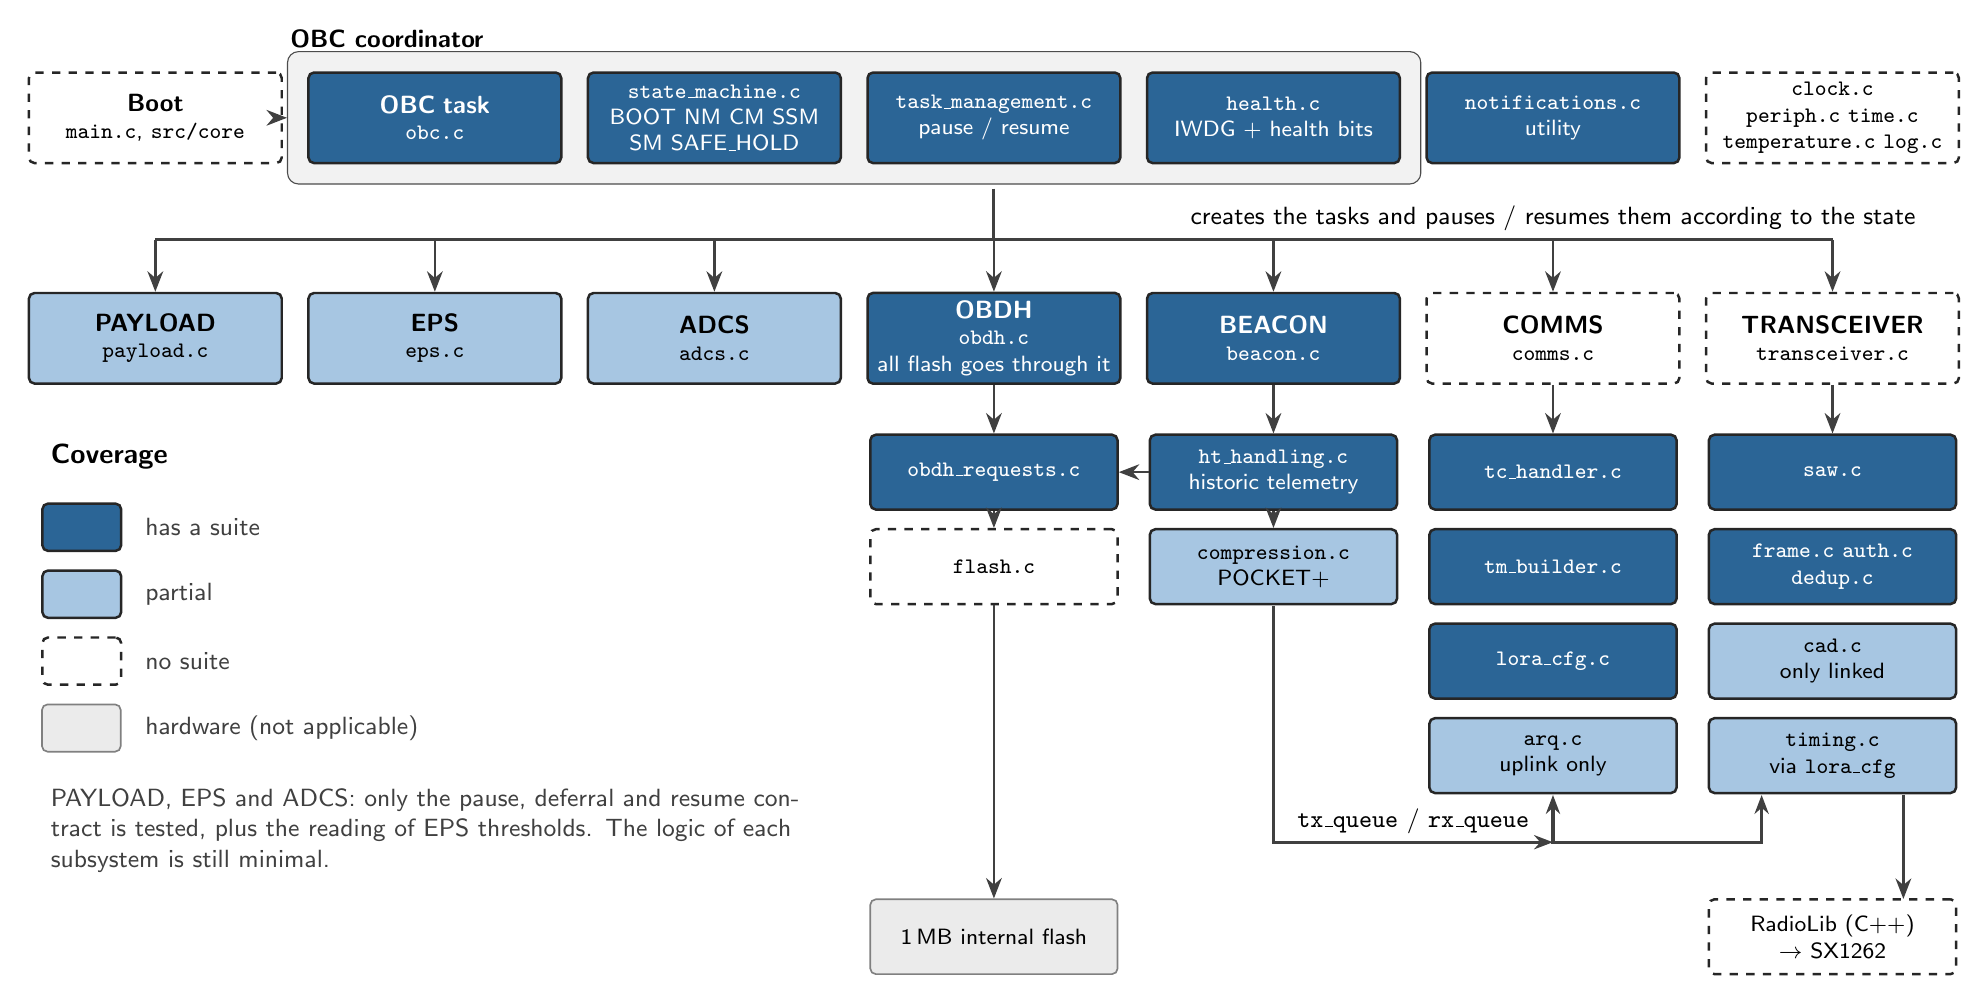
\begin{tikzpicture}[
  t/.style={text width=3.0cm, minimum height=1.15cm, font=\sffamily\footnotesize, inner sep=3pt},
  m/.style={text width=3.0cm, minimum height=0.95cm, font=\sffamily\footnotesize, inner sep=2pt},
  ]
\def\kA{1.65}\def\kB{5.2}\def\kC{8.75}\def\kD{12.3}\def\kE{15.85}\def\kF{19.4}\def\kG{22.95}
% ---- top row: OBC
\node[covnone, t] (main) at (\kA,13.3) {{\small\bfseries Boot}\\\cd{main.c}, \cd{src/core}};
\node[covfull, t] (obc)  at (\kB,13.3) {{\small\bfseries OBC task}\\\cd{obc.c}};
\node[covfull, t] (sm)   at (\kC,13.3) {\cd{state\_machine.c}\\BOOT NM CM SSM\\SM SAFE\_HOLD};
\node[covfull, t] (tm)   at (\kD,13.3) {\cd{task\_management.c}\\pause / resume};
\node[covfull, t] (hl)   at (\kE,13.3) {\cd{health.c}\\IWDG + health bits};
\node[covfull, t] (nt)   at (\kF,13.3) {\cd{notifications.c}\\utility};
\node[covnone, t] (hal)  at (\kG,13.3) {\cd{clock.c} \cd{periph.c} \cd{time.c}\\\cd{temperature.c} \cd{log.c}};
\begin{scope}[on background layer]
  \node[draw=black!70, fill=black!5, rounded corners=4pt, inner sep=2.5mm, fit=(obc)(hl),
        label={[font=\sffamily\bfseries\small, anchor=south west, inner sep=1pt]north west:OBC coordinator}] (obcg) {};
\end{scope}
\draw[arr] (main) -- (obcg.west |- main);

% ---- task bus
\draw[line width=1.1pt, black!75] (\kA,11.75) -- (\kG,11.75);
\draw[line width=1.1pt, black!75] (\kD,12.4) -- (\kD,11.75);
\node[font=\sffamily\small, fill=white, inner sep=1.5pt, anchor=south] at (\kF,11.8)
  {creates the tasks and pauses / resumes them according to the state};

% ---- tasks
\node[covpart, t] (pl) at (\kA,10.5) {{\small\bfseries PAYLOAD}\\\cd{payload.c}};
\node[covpart, t] (ep) at (\kB,10.5) {{\small\bfseries EPS}\\\cd{eps.c}};
\node[covpart, t] (ad) at (\kC,10.5) {{\small\bfseries ADCS}\\\cd{adcs.c}};
\node[covfull, t] (ob) at (\kD,10.5) {{\small\bfseries OBDH}\\\cd{obdh.c}\\all flash goes through it};
\node[covfull, t] (bc) at (\kE,10.5) {{\small\bfseries BEACON}\\\cd{beacon.c}};
\node[covnone, t] (cm) at (\kF,10.5) {{\small\bfseries COMMS}\\\cd{comms.c}};
\node[covnone, t] (tr) at (\kG,10.5) {{\small\bfseries TRANSCEIVER}\\\cd{transceiver.c}};
\foreach \n/\x in {pl/\kA,ep/\kB,ad/\kC,ob/\kD,bc/\kE,cm/\kF,tr/\kG}{ \draw[arr] (\x,11.75) -- (\n.north); }

% ---- submodules
\def\ya{8.8}\def\yb{7.6}\def\yc{6.4}\def\yd{5.2}
\node[covfull, m] (orq) at (\kD,\ya) {\cd{obdh\_requests.c}};
\node[covnone, m] (fl)  at (\kD,\yb) {\cd{flash.c}};
\node[covfull, m] (ht)  at (\kE,\ya) {\cd{ht\_handling.c}\\historic telemetry};
\node[covpart, m] (cp)  at (\kE,\yb) {\cd{compression.c}\\POCKET+};
\node[covfull, m] (tc)  at (\kF,\ya) {\cd{tc\_handler.c}};
\node[covfull, m] (tb)  at (\kF,\yb) {\cd{tm\_builder.c}};
\node[covfull, m] (lc)  at (\kF,\yc) {\cd{lora\_cfg.c}};
\node[covpart, m] (aq)  at (\kF,\yd) {\cd{arq.c}\\uplink only};
\node[covfull, m] (sw)  at (\kG,\ya) {\cd{saw.c}};
\node[covfull, m] (fr)  at (\kG,\yb) {\cd{frame.c} \cd{auth.c} \cd{dedup.c}};
\node[covpart, m] (cad) at (\kG,\yc) {\cd{cad.c}\\only linked};
\node[covpart, m] (tim) at (\kG,\yd) {\cd{timing.c}\\via \cd{lora\_cfg}};

\draw[arr] (ob) -- (orq);
\draw[arr] (orq) -- (fl);
\draw[arr] (bc) -- (ht);
\draw[arr] (ht) -- (cp);
\draw[arr] (ht.west) -- (orq.east);
\draw[arr] (cm) -- (tc);
\draw[arr] (tr) -- (sw);

% ---- hardware
\node[hw, m] (fhw) at (\kD,2.9) {1\,MB internal flash};
\node[covnone, m] (rl) at (\kG,2.9) {RadioLib (C++) \fl{} SX1262};
\draw[arr] (fl) -- (fhw);
\draw[arr] (\kG+0.9,\yd-0.5) -- (\kG+0.9,2.9+0.48);

% ---- queues between COMMS / BEACON and TRANSCEIVER
\draw[line width=1.1pt, black!75, {Stealth[length=2.4mm]}-{Stealth[length=2.4mm]}] (\kF,\yd-0.5) -- (\kF,4.1) -- (\kG-0.9,4.1) -- (\kG-0.9,\yd-0.5);
\draw[line width=1.1pt, black!75, -{Stealth[length=2.4mm]}] (\kE,\yb-0.5) -- (\kE,4.1) -- (\kF,4.1);
\node[font=\sffamily\small, fill=white, inner sep=1.5pt, anchor=south] at ({(\kE+\kF)/2},4.15) {\cd{tx\_queue} / \cd{rx\_queue}};

% ---- legend
\begin{scope}[shift={(0.2,8.9)}]
  \node[font=\sffamily\bfseries, anchor=west] at (0,0.1) {Coverage};
  \node[covfull, minimum width=1.0cm, minimum height=6mm, anchor=west] at (0,-0.8) {};
  \node[note, anchor=west] at (1.2,-0.8) {has a suite};
  \node[covpart, minimum width=1.0cm, minimum height=6mm, anchor=west] at (0,-1.65) {};
  \node[note, anchor=west] at (1.2,-1.65) {partial};
  \node[covnone, minimum width=1.0cm, minimum height=6mm, anchor=west] at (0,-2.5) {};
  \node[note, anchor=west] at (1.2,-2.5) {no suite};
  \node[hw, minimum width=1.0cm, minimum height=6mm, anchor=west] at (0,-3.35) {};
  \node[note, anchor=west] at (1.2,-3.35) {hardware (not applicable)};
  \node[note, anchor=north west, text width=9.6cm] at (0,-4.0)
    {PAYLOAD, EPS and ADCS: only the pause, deferral and resume contract is tested,
     plus the reading of EPS thresholds. The logic of each subsystem is still minimal.};
\end{scope}
\end{tikzpicture}
\caption{Flight software architecture, colored by test coverage. \textbf{What to take
away:} the control core (OBC, state machine, task management, health) and most of
the comms stack are covered. The gaps are at the edges: the TRANSCEIVER task and the COMMS task
(infinite loops), the flash driver, RadioLib, the ARQ downlink and the compressor round trip.}
\label{fig:arch}
\end{slidefig}

% =====================================================================
\section{Known problems (KNOWN BUG)}\label{sec:ki}

\textbf{The rule.} Tests never fix production code. When a test finds
a real bug, it stays written with the correct assertions and the first line of the body is:
\begin{lstlisting}[language=C]
void test_pause_and_resume_pending_together_leaves_task_running(void)
{
    TEST_IGNORE_MESSAGE("KNOWN BUG KI-4: PAUSE wins over RESUME when both are pending; ...");
    /* ... real assertions: what SHOULD happen ... */
}
\end{lstlisting}
Unity marks the test as \cd{IGNORE} and shows the message: the problem stays visible but
the run does not fail. When someone fixes the bug, they only need to delete that line and the
test starts protecting against a regression (figure~\ref{fig:kb}). Each identifier has
a row in the table in \cd{test/README.md}. ``KB'' are the first serious bugs found;
``KI'' are the rest.

\textbf{The two exceptions.} KI-10 and KI-11 (in \cd{test\_ht\_handling}) do not have the
ignore line: their tests fail on purpose. For this reason a full run never comes out green.
Whether to turn them into ignored tests is a pending decision (section~\ref{sec:roadmap}).

\textbf{The ``AC3'' check.} To be sure that a \cd{KNOWN BUG} test tests what it
says, the ignore line is removed, the test is checked to fail for the expected reason, and the line is put
back. This is done and recorded for KB-1, KB-3, KI-4, KI-20, KI-21 and KI-22. It is not recorded for
KI-6, KI-15 (in \cd{test\_beacon}), KI-17, KI-18, KI-19, KI-24 or KI-26.

\begin{figure}[H]
\centering
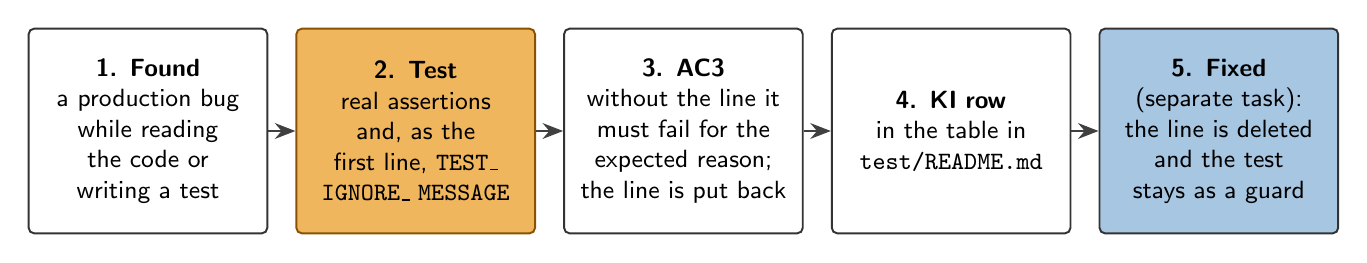
\begin{tikzpicture}[
  ph/.style={box, fill=white, draw=black!80, text width=2.75cm, minimum height=2.6cm, font=\sffamily\small},
  ]
\node[ph] (p1) at (0,0)     {\textbf{1. Found}\\a production bug while reading the code or writing a test};
\node[ph, fill=cFakeL, draw=cFakeD] (p2) at (3.4,0) {\textbf{2. Test}\\real assertions and, as the first line, \cd{TEST\_IGNORE\_} \cd{MESSAGE}};
\node[ph] (p3) at (6.8,0)   {\textbf{3. AC3}\\without the line it must fail for the expected reason; the line is put back};
\node[ph] (p4) at (10.2,0)  {\textbf{4. KI row}\\in the table in \cd{test/README.md}};
\node[ph, fill=cCovPart] (p5) at (13.6,0) {\textbf{5. Fixed}\\(separate task): the line is deleted and the test stays as a guard};
\foreach \a/\b in {p1/p2,p2/p3,p3/p4,p4/p5} \draw[arr] (\a) -- (\b);
\end{tikzpicture}
\caption{Life cycle of a \cd{KNOWN BUG}. \textbf{What to take away:} a known bug is not fixed
from the test work; it is left written as an ignored test that says exactly what should happen,
and fixing it means deleting a single line.}
\label{fig:kb}
\end{figure}

\begingroup
\small
\setlength{\tabcolsep}{4pt}
\renewcommand{\arraystretch}{1.15}
\begin{longtable}{@{}l>{\raggedright\arraybackslash}p{4.1cm}>{\raggedright\arraybackslash}p{7.3cm}>{\raggedright\arraybackslash}p{3.3cm}@{}}
\caption{The 26 known problems, one line each (details in \cd{test/README.md}). Status: \textbf{ignored}
= \cd{KNOWN BUG} test; \textbf{fails} = test that fails on purpose; \textbf{documented} = test that passes and leaves
a record; \textbf{no test}. Line numbers are from the local code (before the \cd{git pull}).}\label{tab:ki}\\
\toprule
ID & Where & Problem & Test status\\
\midrule
\endfirsthead
\toprule
ID & Where & Problem & Test status\\
\midrule
\endhead
\bottomrule
\endfoot
KB-1 & \cd{frame.c} \cd{decode\_raw()} & A frame with LEN 243–255 overflows \cd{payload[242]} before authentication & ignored (\cd{comms\_frame})\\
KB-2 & \cd{transceiver.c:127} & \cd{ack\_buf[8]}, but the ACK takes 16 bytes: stack overflow on every ACK & documented (passes); the transceiver cannot be tested\\
KB-3 & \cd{state\_machine.c} \cd{change\_state()} & Overlapping 4-byte writes: \cd{PREVIOUS\_STATE} always 0 and deployment flags at 0 & ignored ×2 (\cd{state\_machine})\\
KI-4 & \cd{task\_management.c} \cd{tm\_check\_pause()} & PAUSE and RESUME pending at the same time: the task stays paused forever & ignored (\cd{task\_management})\\
KI-5 & \cd{obdh.c} \cd{process\_obdh()} & A paused OBDH does not block: busy loop at priority 5 & ignored (\cd{obdh})\\
KI-6 & \cd{adcs.c} & Private mode bits (0/1) instead of \cd{N\_ADCS\_DESIRED\_STATE\_*} (1/2); \cd{NEW\_TLE} is not handled & ignored (\cd{subsystem\_tasks})\\
KI-7 & \cd{radiolib\_wrapper\_mock.c} & Implements the old API: \cd{build.sh --mock} probably does not compile (not verified) & no test\\
KI-8 & \cd{tc\_handler.c} \cd{UPLOAD\_EPS\_TH}, \cd{UPLOAD\_PL\_CONFIG} & Does not check \cd{frame->len}: saves stale bytes as configuration & ignored ×2 (\cd{tc\_handler})\\
KI-9 & \cd{task\_management.c} \cd{tm\_create\_tasks()} & Returns the \cd{xTaskCreate} code, not \cd{pdFAIL} (harmless) & documented (passes)\\
KI-10 & \cd{ht\_handling.c} \cd{ht\_init()} & After the 32-bit counter wraps around it picks the wrong oldest slot & \textbf{fails} (\cd{ht\_handling})\\
KI-11 & \cd{ht\_handling.c} \cd{ht\_store\_block()} & A bad page is retried forever: the history stops being saved & \textbf{fails} (\cd{ht\_handling})\\
KI-12 & \cd{obdh.c:65-66} & Deferred notifications are lost (\cd{N\_OBDH\_CLEAR\_FLASH}, \cd{N\_OBDH\_CLEAR\_HT}) & no test (warning in \cd{tc\_handler})\\
KI-13 & \cd{health.c:175} \cd{system\_health()} & Missing NULL check if called before \cd{health\_init()} & no test\\
KI-14 & \cd{obdh\_requests} \fl{} \cd{obdh} \fl{} \cd{flash} & \cd{size\_t len} is truncated to \cd{uint16\_t} & no test\\
KI-15 & \cd{TC\_SET\_BEACON\_PERIOD} \fl{} \cd{beacon\_set\_period()} & Period 0: \cd{configASSERT} hangs the OBC until the IWDG fires & ignored ×2 (\cd{tc\_handler}, \cd{beacon})\\
KI-16 & \cd{tc\_handler.c}, ARQ TCs & If the ARQ is busy, \cd{NACK\_BUSY} is not sent: the ground waits for a transfer that never starts & ignored (\cd{tc\_handler})\\
KI-17 & \cd{beacon.c} + \cd{obc.c} & The uptime comes from the RTC: syncing the time after boot corrupts it & ignored (\cd{beacon})\\
KI-18 & \cd{lora\_cfg.c} \cd{validate()} + \cd{timing.c} & Unbounded preamble: the time on air overflows \cd{uint32} & ignored (\cd{lora\_cfg})\\
KI-19 & \cd{timing.c:309}, \cd{arq.c} & The ACK timeout is computed with an 8-byte ACK; it is 16 bytes & ignored (\cd{lora\_cfg})\\
KI-20 & \cd{arq.c:460}, \cd{arq.c:538-539} & \cd{WINDOW\_SIZE = 0} is accepted: modulo by zero (UBSan aborts) & ignored (\cd{arq})\\
KI-21 & \cd{arq.c:453-457} & A transfer type other than arming is only written to the log & ignored (\cd{arq})\\
KI-22 & \cd{arq.c} + \cd{flash.h} & The uplink is not limited to the region: it can overwrite up to \cd{BOOT\_TIME\_ADDR} & ignored (\cd{arq})\\
KI-23 & \cd{arq.c:87}, \cd{arq.c:118-119} & The HK history downlink reads \cd{TELEMETRY\_ADDR} (old), never the HT queue & no test (downlink pending)\\
KI-24 & \cd{saw.c:20}, \cd{saw.c:92-99} & \cd{own\_type} is ignored when matching ACK/NACK & ignored (\cd{saw})\\
KI-25 & \cd{obc.c:112-121} & The restart and update-time bits are empty \cd{if}s (not implemented) & documented (note in \cd{obc})\\
KI-26 & \cd{state\_machine.c} \cd{change\_state()} & A transition to the current state pauses and resumes everything and does 2 writes & ignored (\cd{obc})\\
\end{longtable}
\endgroup

Count: 16 identifiers have ignored tests (19 tests in total, because KB-3, KI-8 and KI-15
have two each); 2 have failing tests (KI-10, KI-11); 3 are documented by a passing
test or a note (KB-2, KI-9, KI-25); and 4 have no test at all (KI-7, KI-12, KI-13, KI-14), plus
KI-23, which waits for the ARQ downlink tests.

In addition, while writing \cd{test\_arq} and \cd{test\_ht\_compression}, three more things
were seen that look like bugs and that have neither a test nor an identifier yet:
\begin{itemize}
\item in \cd{arq.c}, a block more than 64 positions above the first missing one is not
  marked in the bitmap, and a duplicate is counted twice;
\item in \cd{arq.c}, a block longer than the announced size overwrites the next one in the
  reassembly buffer;
\item \cd{startPocket()} does not reset \cd{protectionLevel} or \cd{sizeOldCompressedPacket}
  (harmless with protection level 1).
\end{itemize}

\clearpage
% =====================================================================
\section{Status, weak points and roadmap}\label{sec:roadmap}

\subsection{What comes first: integrating the remote changes}

On \cd{origin/obdh-compression} there are two commits that are not yet in the local copy:
\cd{7bf67b0} (\emph{Flash step 1: memory map, driver region guard, 256 KB code limit, HT
move}) and \cd{7314944}. They touch 20 files in \cd{src/}, \cd{include/} and \cd{cmake/}, and none
in \cd{test/}. For this reason the \cd{git pull} will not give conflicts, but it \textbf{will very
probably leave some suites unable to compile}, because they change exactly the interfaces that the
fakes replace.

\avis{Forecast, not a verified fact.}{The following table was made by reading the commit message and the diff. The
\cd{pull} has not been done and the tests have not been run with these changes.}

\begin{table}[H]
\centering\small
\begin{tabularx}{\textwidth}{@{}>{\raggedright\arraybackslash}X>{\raggedright\arraybackslash}X@{}}
\toprule
What changes in the flight code & What will need review in the tests\\
\midrule
\cd{obdh\_read\_request}, \cd{obdh\_program\_request} and \cd{obdh\_erase\_program\_request} go from taking an absolute
address to taking \cd{(region, offset)}. \cd{obdh\_write\_request} stays with old-map addresses
and \cd{obdh\_read\_old\_request} appears. &
\cd{fake\_obdh\_requests} and \cd{mock\_obdh\_requests} (the signatures), and the suites that check addresses:
\cd{test\_tc\_handler}, \cd{test\_arq}, \cd{test\_subsystem\_tasks}, \cd{test\_beacon}.\\
The driver (\cd{flash\_read}, \cd{flash\_program}, \cd{flash\_erase\_page}) takes region and offset and rejects any range outside the region. &
\cd{fake\_flash\_driver} and \cd{test\_obdh}.\\
Historic telemetry moves from 8\,KB at \cd{0x080FE000} to its own 64\,KB region. &
\cd{stubs\_project/flash.h}, \cd{fake\_flash\_memory}, \cd{test\_ht\_handling}, \cd{test\_ht\_compression}.\\
New memory map in \cd{include/utils/flash\_map.h}; the \emph{linker} limits the code to 256\,KB. &
The address constants used by the suites. The current firmware (82\,KB) fits with plenty of room.\\
New modules: \cd{param\_store.c} (629 lines) and \cd{crc32.c}. & They have no suite.\\
\cd{arq.c} changes (fills rejected reads with \cd{0xFF}). & The line numbers for KI-19 to KI-23 shift; it must be checked again whether KI-22 and KI-23 still hold.\\
\bottomrule
\end{tabularx}
\caption{Expected impact of the remote commits on the test infrastructure.}
\label{tab:remote}
\end{table}

The safe order is: first commit the local work (so there is a point to go back to),
then the \cd{pull}, and then adapt the fakes and suites until the full run returns
to today's state. It is a good moment to decide whether \cd{fake\_obdh\_requests} becomes
strict, because it will have to be rewritten anyway.

\subsection{Weak points found by the external review}

An external review (read only) found 19 points (F1–F19). Some are already
resolved; the ``Status'' column is the current status checked in the repo.

\begingroup
\small
\setlength{\tabcolsep}{4pt}
\renewcommand{\arraystretch}{1.15}
\begin{longtable}{@{}l l>{\raggedright\arraybackslash}p{9.6cm}>{\raggedright\arraybackslash}p{4.3cm}@{}}
\toprule
ID & Sev. & Weak point & Status\\
\midrule
\endfirsthead
\toprule
ID & Sev. & Weak point & Status\\
\midrule
\endhead
\bottomrule
\endfoot
F1 & high & \cd{test\_torn\_write\_recovery} does not test a half-done write: the cut comes after the erase and before anything is programmed & open\\
F2 & high & The compressor is a mock in \cd{test\_ht\_handling} and \cd{test\_beacon} & partly: \cd{test\_ht\_compression} uses the real one; the round trip is missing\\
F3 & med. & Assertions that only check what the fake wrote; the TC \fl{} effect chain is not closed because the target task is a stub (e.g. KI-12) & open\\
F4 & med. & KI-10 and KI-11 in red: a real regression cannot be told apart from the expected failures & \textbf{decision pending}\\
F5 & med. & The reset of the \cd{static}s is copied into every suite; there are function-local \cd{static}s in \cd{tc\_handler.c} that cannot be reset & open\\
F6 & med. & The fake timers accept period 0 (the real FreeRTOS does \cd{configASSERT}) & open\\
F7 & high & \cd{fake\_obdh\_requests} is permissive (no alignment or erase check) and 7 suites use it & \textbf{decision pending}\\
F8 & med. & Three flash models with different rules; \cd{fake\_flash\_driver} has no power cut & open\\
F9 & med. & Single thread: it does not model races, priorities, ISRs or stacks; the host is 64-bit & design limit\\
F10 & low & The \emph{weak} symbols of \cd{fake\_comms\_env} can stop counting without warning if the link changes & open\\
F11 & high & No suite: \cd{transceiver.c} (no test fails for KB-2), \cd{comms.c}, \cd{flash.c}; ARQ downlink & partly: \cd{test\_arq} covers the uplink\\
F12 & med. & The OBDH is paused on every state transition and could block a flash client & \textbf{suspected, not confirmed}\\
F13 & med. & No per-suite timeout in \cd{ctest}; no \cd{-Werror} & timeout resolved (60\,s); \cd{-Werror} not\\
F14 & med. & There is no CI & \textbf{decision pending}\\
F15 & med. & Outdated documentation & resolved in \cd{test/README.md} and \cd{docs/testing/}; \cd{CLAUDE.md} remains\\
F16 & med. & The firmware image carries a fixed development PSK with no warning & open\\
F17 & low & \cd{.gitattributes} not committed & open\\
F18 & low & \cd{run\_tests.sh}: \cd{-f} without a suite name turns into a regex; unclear messages & open\\
F19 & low & The ARM toolchain is downloaded without checking the checksum & open\\
\end{longtable}
\endgroup

\textbf{About F12 (suspected).} The code confirms half of it: \cd{change\_state()} calls
\cd{tm\_pause\_tasks(tasks\_for\_state(old\_state))}, and \cd{tasks\_for\_state()} includes
\cd{TM\_TASK\_OBDH} in every state, so the OBDH receives \cd{N\_TASK\_PAUSE} on every transition
(this contradicts the sentence about KI-5 in \cd{test/README.md} that says it is ``never paused''). What is
\emph{not} confirmed is the consequence: that a task blocked in \cd{obdh\_submit\_request()}
(waiting \cd{portMAX\_DELAY} on index 1) cannot get a reply because of the pause and ends up in a timeout or
restarted by the watchdog. No suite tests this: the ones that do transitions use
\cd{fake\_obdh\_requests}, which has no OBDH task. A test is needed before treating it as a bug.

\subsection{Roadmap}

Figure~\ref{fig:roadmap} orders the pending work by priority. The cards with a red border
and the DECISION label wait for the owner to decide; they must not be done without that
decision. The arrows mark dependencies.

% ---------------------------------------------------------------- FIGURE: roadmap
\begin{slidefig}
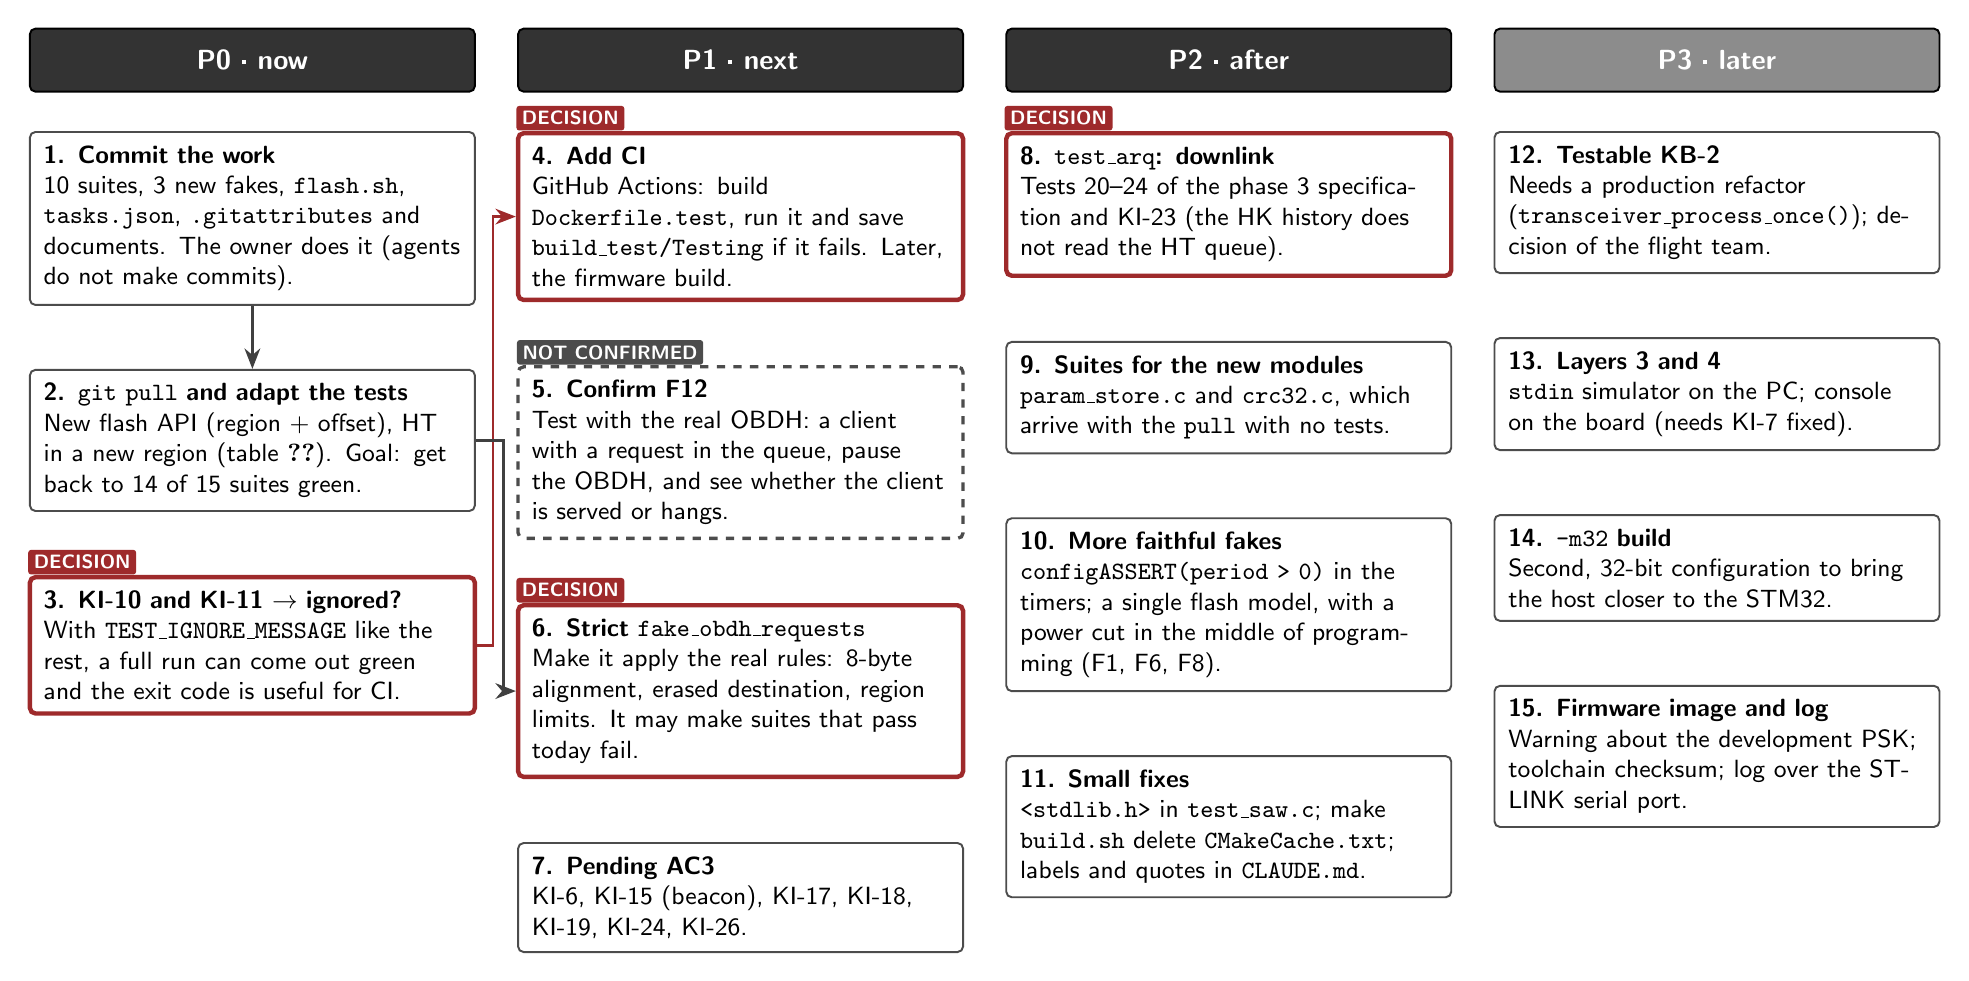
\begin{tikzpicture}[
  colh/.style={box, fill=black!80, text=white, text width=5.3cm, font=\sffamily\bfseries, inner sep=5pt},
  ]
\def\xa{2.95}\def\xb{9.15}\def\xc{15.35}\def\xd{21.55}
\node[colh] (h0) at (\xa,0) {P0 · now};
\node[colh] (h1) at (\xb,0) {P1 · next};
\node[colh] (h2) at (\xc,0) {P2 · after};
\node[colh, fill=black!45] (h3) at (\xd,0) {P3 · later};

% P0
\node[card, anchor=north] (c1) at (\xa,-0.9) {\textbf{1. Commit the work}\\10 suites, 3 new fakes, \cd{flash.sh}, \cd{tasks.json},
  \cd{.gitattributes} and documents. The owner does it (agents do not make commits).};
\node[card, anchor=north] (c2) [below=8mm of c1] {\textbf{2. \cd{git pull} and adapt the tests}\\New flash API (region + offset), HT in a new region
  (table~\ref{tab:remote}). Goal: get back to 14 of 15 suites green.};
\node[deccard, anchor=north] (c3) [below=8mm of c2] {\textbf{3. KI-10 and KI-11 \fl{} ignored?}\\With \cd{TEST\_IGNORE\_MESSAGE} like the rest, a full run
  can come out green and the exit code is useful for CI.};
\node[tag, anchor=south west] at (c3.north west) {DECISION};

% P1
\node[deccard, anchor=north] (c4) at (\xb,-0.9) {\textbf{4. Add CI}\\GitHub Actions: build \cd{Dockerfile.test}, run it and save
  \cd{build\_test/Testing} if it fails. Later, the firmware build.};
\node[tag, anchor=south west] at (c4.north west) {DECISION};
\node[card, anchor=north, draw=black!70, dashed, line width=1.2pt] (c5) [below=8mm of c4] {\textbf{5. Confirm F12}\\Test with the real OBDH: a client with a
  request in the queue, pause the OBDH, and see whether the client is served or hangs.};
\node[tagu, anchor=south west] at (c5.north west) {NOT CONFIRMED};
\node[deccard, anchor=north] (c6) [below=8mm of c5] {\textbf{6. Strict \cd{fake\_obdh\_requests}}\\Make it apply the real rules: 8-byte alignment, erased
  destination, region limits. It may make suites that pass today fail.};
\node[tag, anchor=south west] at (c6.north west) {DECISION};
\node[card, anchor=north] (c7) [below=8mm of c6] {\textbf{7. Pending AC3}\\KI-6, KI-15 (beacon), KI-17, KI-18, KI-19, KI-24, KI-26.};

% P2
\node[deccard, anchor=north] (c8) at (\xc,-0.9) {\textbf{8. \cd{test\_arq}: downlink}\\Tests 20–24 of the phase 3 specification and KI-23 (the HK history does not
  read the HT queue).};
\node[tag, anchor=south west] at (c8.north west) {DECISION};
\node[card, anchor=north] (c9) [below=8mm of c8] {\textbf{9. Suites for the new modules}\\\cd{param\_store.c} and \cd{crc32.c}, which arrive with the
  \cd{pull} with no tests.};
\node[card, anchor=north] (c10) [below=8mm of c9] {\textbf{10. More faithful fakes}\\\cd{configASSERT(period > 0)} in the timers; a single
  flash model, with a power cut in the middle of programming (F1, F6, F8).};
\node[card, anchor=north] (c11) [below=8mm of c10] {\textbf{11. Small fixes}\\\cd{<stdlib.h>} in \cd{test\_saw.c}; make \cd{build.sh} delete
  \cd{CMakeCache.txt}; labels and quotes in \cd{CLAUDE.md}.};

% P3
\node[card, anchor=north] (c12) at (\xd,-0.9) {\textbf{12. Testable KB-2}\\Needs a production refactor (\cd{transceiver\_process\_once()}); decision of the flight team.};
\node[card, anchor=north] (c13) [below=8mm of c12] {\textbf{13. Layers 3 and 4}\\\cd{stdin} simulator on the PC; console on the board (needs KI-7 fixed).};
\node[card, anchor=north] (c14) [below=8mm of c13] {\textbf{14. \cd{-m32} build}\\Second, 32-bit configuration to bring the host closer to the STM32.};
\node[card, anchor=north] (c15) [below=8mm of c14] {\textbf{15. Firmware image and log}\\Warning about the development PSK; toolchain checksum;
  log over the ST-LINK serial port.};

\draw[arr] (c1) -- (c2);
\draw[arr, cWarn] (c3.east) -- ++(0.2,0) |- (c4.west);
\draw[arr] (c2.east) -- ++(0.35,0) |- (c6.west);
\end{tikzpicture}
\caption{Roadmap by priority. \textbf{What to take away:} the first step is to commit what
already exists; the second is to bring in the remote flash changes and adapt the tests to them. Four items wait for a
decision from the owner (red border), and the possible problem with the paused OBDH must be confirmed with a
test before it is treated as a bug.}
\label{fig:roadmap}
\end{slidefig}

% =====================================================================
\appendix
\section{Command cheat sheet}\label{sec:xuleta}

All from the repository root, in PowerShell, with Docker Desktop open.

\textbf{Once per PC (or when the matching Dockerfile changes)}
\begin{lstlisting}
docker build -t pocat-build-env .
docker build -t pocat-tests -f Dockerfile.test .
\end{lstlisting}

\textbf{Firmware}
\begin{lstlisting}
docker run --rm -v "${PWD}:/app" pocat-build-env                          # build
docker run --rm -v "${PWD}:/app" pocat-build-env bash build.sh --clean    # from scratch
docker run --rm -v "${PWD}:/app" pocat-build-env arm-none-eabi-size build/pocat_lektron_sw.elf
\end{lstlisting}

\textbf{Board}
\begin{lstlisting}
& "C:\Program Files\Git\bin\bash.exe" flash.sh             # flash
& "C:\Program Files\Git\bin\bash.exe" flash.sh --dry-run   # only shows what it would do
\end{lstlisting}
In VS Code: \cd{F5} (build, flash and run), \cd{Ctrl+Shift+B} (build) and
\emph{Terminal > Run Task...} (the rest).

\textbf{Tests}
\begin{lstlisting}
docker run --rm -v "${PWD}:/app" pocat-tests                               # everything
docker run --rm -v "${PWD}:/app" pocat-tests --list                        # list of suites
docker run --rm -v "${PWD}:/app" pocat-tests --label obc                   # one label
docker run --rm -v "${PWD}:/app" pocat-tests state_machine                 # suites by name
docker run --rm -v "${PWD}:/app" pocat-tests test_state_machine -l         # tests of one suite
docker run --rm -v "${PWD}:/app" pocat-tests test_state_machine -f NM_to_SM  # a filter
docker run --rm -v "${PWD}:/app" pocat-tests test_tc_handler -f TC_REQUEST_HK
\end{lstlisting}

\textbf{This document} (tests + figures + PDF; appendix~\ref{sec:rebuild})
\begin{lstlisting}
& "C:\Program Files\Git\bin\bash.exe" docs/testing/overview/build-docs.sh
& "C:\Program Files\Git\bin\bash.exe" docs/testing/overview/build-docs.sh --no-tests   # keep last results
\end{lstlisting}

\textbf{Reminders}
\begin{itemize}
\item The quotes in \cd{"\PWD:/app"} are needed: the repository path has spaces.
\item A full test run ends with an error while KI-10 and KI-11 fail on purpose;
  what matters is that nothing else fails.
\item Never build the default target inside \cd{build\_test/}.
\item \cd{psk.h}, \cd{build/} and \cd{build\_test/} are generated: do not edit them or commit them.
\item Before rebuilding this PDF, close it in the viewer.
\end{itemize}

% =====================================================================
\clearpage
\section{Rebuilding this document}\label{sec:rebuild}

The PDF is built by one script, \cd{docs/testing/overview/build-docs.sh}, which runs three
throwaway containers in a row (figure~\ref{fig:docbuild}). Run it from the repository root, with
Docker Desktop open:
\begin{lstlisting}
& "C:\Program Files\Git\bin\bash.exe" docs/testing/overview/build-docs.sh
\end{lstlisting}

\begin{enumerate}
\item \textbf{Tests.} The \cd{pocat-tests} image runs \cd{tools/collect-test-results.sh}: it builds
  \cd{pocat\_tests}, runs every suite binary listed by \cd{ctest -N}, and turns the Unity lines
  (\cd{file:line:test:PASS|FAIL|IGNORE}) into the \cd{\textbackslash TR...} macros in
  \cd{generated/test-results.tex}. A failing test does not stop the build: it is data for the PDF.
\item \textbf{Figures.} The \cd{rlespinasse/drawio-export} image exports every
  \cd{figures/*.drawio} to a cropped PDF in \cd{figures/pdf/}. To change a figure, open the
  \cd{.drawio} file in draw.io (desktop app, VS Code extension or \cd{app.diagrams.net}), save,
  and rebuild.
\item \textbf{PDF.} The \cd{dxjoke/tectonic-docker} image typesets this file. The first run downloads
  the LaTeX packages it needs, so it needs internet.
\end{enumerate}

Options: \cd{--no-tests} reuses the last \cd{generated/test-results.tex} (fast, for text-only changes);
\cd{--no-figures} skips the draw.io export. Everything the script writes (\cd{generated/},
\cd{figures/pdf/}) is ignored by git; the sources (\cd{.tex}, \cd{.drawio}, scripts) are not.

\textbf{What is automatic and what is not.} Only the test numbers follow the code: the summary
tiles and the status bullet in section~\ref{sec:resum}. The rest of the
text (known-issues analysis, roadmap, the terminal outputs) is a hand-checked snapshot of
13/11/2026. When the code changes in a way that matters, that prose has to be updated by hand.

\begin{figure}[H]
\centering
\drawio[\linewidth]{docs-pipeline}
\caption{What \cd{build-docs.sh} does (draw.io: \cd{figures/docs-pipeline.drawio}). \textbf{What to take
away:} one command takes the repository as it is right now and produces a PDF whose test numbers
come from a real run on that code, and whose figures come from the editable \cd{.drawio} files.}
\label{fig:docbuild}
\end{figure}

\end{document}
